\section{Messen von Kondensatoren}
Die Messung von Kapazitätswerten wird nach allen anderen Messungen als separater Teil mit einer Ladezeitmessung 
durchgeführt.
Die Originalsoftware vom Markus F. hat das mit einer Programmschleife gemacht, die den betreffenden digitalen
Eingangs-Pin bis zu einer Signaländerung gelesen hat und dabei die Schleifendurchläufe gezählt.
Dies hat den Nachteil, dass die Auflösung der Zeitmessung begrenzt ist durch die Gesamtzeit eines Schleifendurchlaufs.
Dies wurde üblicherweise in allen sechs Kombinationsmöglichkeiten für die drei Testpins durchgeführt.
Die aktuelle Software benutzt zwei verschiedene Möglichkeiten, um die Ladezeit in nur drei
Kombinationsmöglichkeiten für die drei Testpins zu erhalten.
Die positive Seite ist nun immer die höhere Testpin-Nummer.
Nur wenn die Kapazität zusammen mit einer parallel geschalteten Diode gemessen wird,
kann die Polarität die andere Richtung haben.

\subsection{Entladen der Kondensatoren}
Sie sollten die Kapazitäten immer entladen, bevor sie mit dem Tester verbunden werden.
Bevor irgendein Test gestartet wird, wird der Kondensator vom Tester immer noch einmal entladen.
Wenn die Spannung unter 1300mV ist, wird der Kondensator dafür mit den angeschlossenen ADC-Ports (Port C) kurzgeschlossen.
Ich glaube das ist in Ordnung, weil jeder Portausgang einen Innenwiderstand von ungefähr \(20\Omega\) hat.
Die Abbildung 149 (Seite 258) im Atmega8-Datenblatt \cite{ATmega8} zeigt einen Spannungsabfall an Ausgabe-Pins von bis zu 2V.
Natürlich kann ich nicht garantieren, dass kein Schaden auftreten kann.
Ich habe die Funktion mit Kondensatoren von mehr als \(15 mF\) sehr oft getestet und ich habe noch nie ein Problem bemerkt.
Der Strom sollte unter der spezifizierten Grenze von 40mA bleiben und reduziert sich schnell durch die Entladung.
Natürlich kann ein Schaden entstehen, wenn Sie einen (Hochvolt-) Kondensator nicht vollständig entladen, bevor Sie ihn an den Tester anschließen.

\subsection{Messung von großen Kapazitäten}
\label{sec:bigcap}
Eine Seite des Kondensators ist mit GND verbunden. Die andere Seite wird über den \(680\Omega\)-Widerstand für 10ms mit VCC verbunden.
Danach wird dieser Messpin auf Eingang geschaltet (hochohmig).
Nach diesem Strompuls wird die Spannung am Kondensator stromlos gemessen.
Wenn die Spannung noch nicht den Minimalwert von 300mV erreicht hat, wird dieser Ladepuls bis zu weiteren 499 Mal wiederholt.
Wenn nach 127 Pulsen (ungefähr 2s) noch nicht eine Minimalspannung von 75mV erreicht ist, wird der Ladevorgang abgebrochen,
 weil die 300mV mit den verbleibenden Ladepulsen nie erreicht werden wird.
Abbildung~\ref{fig:bigcap1} zeigt die drei Phasen der Kapazitätsbestimmung eines Kondensators.
Der Kapazitätswert wird dann berechnet aus der Ladepuls-Anzahl und der erreichten Ladespannung über eine Tabelle.
Die Tabelle enthält mit einem Spannungsabstand von 25mV die Faktoren, um aus der Ladezeit und der Spannung 
den Kapazitätswert zu bestimmen. 
Zwischenwerte der Spannung werden interpoliert.

\begin{figure}[H]
\centering

\includegraphics[]{../FIG/Bigcap.eps}
\caption{Kondensator-Entladung und -Ladung mit 10ms Ladepulsen bis zur Spannung \textgreater 300mV}
\label{fig:bigcap1}
\end{figure}

Wegen der niedrigen Ladespannung wird die Messung viel schneller als bei der ursprünglichen Softwareversion,
weil dieser Vorteil auch bei der Entladung wirkt. So können auch grössere Kondensatoren gemessen werden.
Zusätzlich stört in den meisten Fällen eine parallel geschaltete Diode nicht die Messung, weil die Schwellspannung
der Diode nicht erreicht wird.
Abbildung~\ref{pic:c229} zeigt das Laden und Entladen eines \(229\mu F\) großen Kondensators.
Das flache Dach der Messkurve bis zum Entladebeginn ist durch die Messzeit und Berechnungszeit des ATmega verursacht.
Abbildung~\ref{pic:c5mF} zeigt die gleiche Messung mit einem~\(5mF\)-Kondensator,
beachte wie die Messzeit inklusive Entladung auf ungefähr 1,5 Sekunden angewachsen ist.
Das letzte Beispiel in Abbildung~\ref{pic:c15mF} zeigt die Messung eines \(15mF\)-Kondensators.

\begin{figure}[H]
  \begin{subfigure}[b]{9cm}
    \centering
    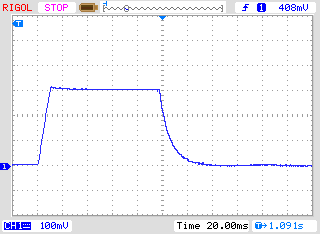
\includegraphics[width=9cm]{../PNG/charge_229uF.png}
    \caption{\(229\mu F\)-Kondensator}
    \label{pic:c229}
  \end{subfigure}
  ~
  \begin{subfigure}[b]{9cm}
    \centering
    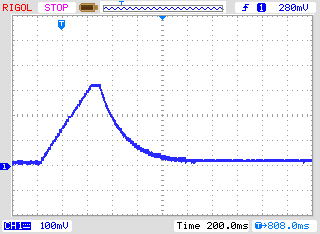
\includegraphics[width=9cm]{../PNG/charge_5mF.png}
    \caption{\(5mF\)-Kondensator}
    \label{pic:c5mF}
  \end{subfigure}
  \caption{Laden und Entladen von großen Kondensatoren für die Messung}
\end{figure}

\begin{figure}[H]
  \centering
    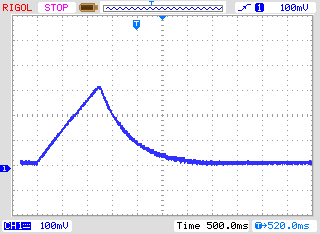
\includegraphics[]{../PNG/charge_15mF.png}
  \caption{Laden und Entladen eines \(15mF\)-Kondensators für die Messung}
  \label{pic:c15mF}
\end{figure}

Nach dieser Kondensatormessung wird die Selbstentladung des Kondensators untersucht, indem der
Spannungsverlust in einer der Ladezeit proportionalen Zeit untersucht wird.
Der gemessene Kapazitätswert wird entsprechend korrigiert. Ein Test mit einer Parallelschaltung von
einem \(68 \mu F\)-Kondensator mit einem \(2.2 k\Omega\)-Widerstand zeigt die
Wirksamkeit der Methode. Der ermittelte Kapazitätswert ohne den Widerstand beträgt \(66.5 \mu F\),
mit dem parallelen \(2.2 k\Omega\) Widerstand wird ein Kapazitätswert von \(65.3 \mu F\) gemessen.
Zum Vergleich möchte ich die entsprechenden Ergebnisse mit einem Peaktech 3315 Multimeter angeben.
Ohne den Widerstand wird eine Kapazität von \(68.2 \mu F\) gemessen, mit dem parallelen \(2.2 k\Omega\)
Widerstand wird aber \(192 \mu F\) mit dem Multimeter gemessen.

\subsection{Messen von kleinen Kapazitäten}
Wenn der erste 10 ms Ladepuls den Kondensator zu hoch aufgeladen hat, wird eine andere Messtechnik benutzt.
Der ATmega-Mikrocontroller hat einen eingebauten 16-Bit-Zähler, der bei voller Taktfrequenz (1MHz oder 8MHz) arbeiten kann.
Diese Zähler hat auch die Fähigkeit aufgrund eines externen Ereignisses den Zählerstand zu sichern.
Dieses Ereignis kann auch das Ausgangs-Signal des Komparators sein.
Der Komparator kann mit jedem ADC-Eingangspin und der Spannungsreferenz (Band Gap Reference) arbeiten.
Das Schaltbild~\ref{fig:comparat} zeigt ein vereinfachtes Diagram der Messsituation.
So entlade ich den Kondensator, bereite den Komparator für den richtigen Pin Eingang vor, starte den Zähler bei 0 und
starte sofort das Laden des Kondensators.
Dabei ist eine Seite des Kondensators mit GND, die andere Seite über den \(470k\Omega\)-Widerstand mit VCC verbunden.
Nun prüfe ich in einer Programm-Schleife, ob der Zähler ein Überlauf-Ereignis (overflow) oder ein
 externes Ereignis (input capture) meldet.
Die Überlauf-Ereignisse zähle ich, bis ich ein externes Ereignis feststelle.
In diesem Fall halte ich den Zähler an und prüfe, ob ich noch einen zusätzlichen Überlauf zählen muss, 
weil der Zähler nicht mit dem externen Ereignis (input capture) angehalten werden kann.


Der Zählerstand des externen Ereignisses bildet zusammen mit dem Überlaufzähler die Gesamtzeit, aus der die
Kapazität mit einem Faktor bestimmt wird.
Die aktuelle Software kann eine Tabelle mit der theoretischen Abhängigkeit der Ladezeit in Bezug auf die gemessene
Komparator-Spannung berücksichtigen.
Die Tabelle besitzt Einträge in Schritten von 50mV, die Ergebnisse werden entsprechend der aktuellen Referenz-Spannung interpoliert.
Diese Tabelle wird nur mit der Makefile Option WITH\_AUTO\_REF aktiviert.
Vom Kapazitätswert ziehe ich eine experimentell herausgefundene vordefinierte Konstante oder eine im Selbsttest
herausgefundene Konstante ab, um den Messwerte-Offset zu beseitigen.
Ich weiß nicht, ob die vordefinierte Konstante für andere Leiterplatten angepasst werden muss.
Mit einem Selbsttest bei gesetzter AUTO\_CAL Option wird diese Anpassung automatisch erledigt.

Ich habe bemerkt, dass die Referenz-Spannung meistens etwas zu klein gemessen wird,
 deshalb kann man einen Zusatz mit der Makefile Option REF\_C\_KORR angeben.
Nach der Kalibration mit der AUTO\_CAL option ist der REF\_C\_KORR Wert nur ein Zusatz zu der automatisch
gefundenen Differenz zwischen geladener Kondensator-Spannung und der internen Referenz-Spannung.
Die gemessene Referenz-Spannung wird dann mit dem Korrekturwert (in mV) korrigiert (addiert).
Wenn die Option WITH\_AUTO\_REF nicht benutzt wird, werden die Referenz-Spannungen entsprechend den Angaben in den
Datenblättern ~\cite{ATmega8}~\cite{ATmega168} der ATmega8, ATmega168 und ATmega328 berücksichtigt.
Eine Beispielmessung von diesem Typ ist in Abbildung~\ref{pic:c22uF} dargestellt.
Die Messzeit für den \(22 \mu F\)-Kondensator beträgt ungefähr 2,6s weil der \(470k\Omega\)-Widerstand für das Laden benutzt wird.
Aber das Entladen geht in diesem Fall viel schneller als das Laden.

\begin{figure}[H]
\centering

\includegraphics[]{../FIG/Comparat.eps}
\caption{Messung kleiner Kapazitätswerte mit dem Komparator}
\label{fig:comparat}
\end{figure}

\begin{figure}[H]
  \centering
    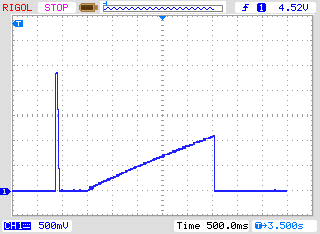
\includegraphics[]{../PNG/charge_22uF.png}
  \caption{Laden und Entladen eines \(22\mu F\)-Kondensators für die Messung}
  \label{pic:c22uF}
\end{figure}


Im Prinzip kann diese Technik auch mit dem \(680\Omega\)-Widerstand benutzt werden,
aber weil während dem Komparatorbetrieb der ADC nicht benutzt werden kann, besteht keine
Möglichkeit die Ladespannung zu beobachten bis der Komparator angehalten wird.
Wenn eine unentdeckte Diode mit dem Kondensator parallelgeschaltet ist, kann der Ladestrom
von der Diode aufgenommen werden (Schwellspannung) und die Referenz-Spannung würde nie erreicht.
Dieser Konzeptfehler wird mit der Methode vermieden, die in der aktuellen Software für große Kondensatoren in Kapitel~\ref{sec:bigcap}
verwendet wird.

\subsection{Messen des äquivalenten Serienwiderstandes ESR, Methode 1}
Der ESR \cite{ESR} stellt zum Beispiel ein Maß für die Alterung von Elektrolyt-Kondensatoren dar.
Die Abbildung~\ref{fig:Cap_equiv} zeigt ein Ersatzschaltbild eines Kondensators.
Der Widerstand \(Rp\) stellt den Isolationswiderstand des Kondensators dar, \(ESL\) die äquivalente
Serieninduktivität und der Widerstand \(ESR\) stellt den äquivalenten Serienwiderstand dar.
Bei Kondensatoren mit mehr als \(0.45 \mu F\) wird versucht, den Serienwiderstand von Kondensatoren zu messen.
Bei mehr als \(3.6 \mu F\) wird dazu die normale Taktrate von \(125 kHz\) für den Analog-Digital Wandler benutzt.
Bei kleineren Kapazitäten wird eine erhöhte Taktrate von \(500 kHz\) benutzt, um die Messung zu beschleunigen.
Die Genauigkeit der ADC-Ergebnisse wird bei der höheren Taktrate zwar schlechter, aber die größeren ESR-Werte
bei kleineren Kondensatoren mildern die Auswirkung dieses Genauigkeitsverlusts ab. 
Andererseits ist sonst nach diesem Verfahren keine ESR-Messung für Kondensatoren unter \(1.8 \mu F\) möglich.

\begin{figure}[H]
  \centering
    
\includegraphics[]{../FIG/Cap_equiv.eps}
  \caption{Ersatzschaltbild eines Kondensators}
  \label{fig:Cap_equiv}
\end{figure}

Genau genommen ist der ESR eines Kondensators abhängig von der Betriebsfrequenz und der Temperatur.
Üblicherweise wird der mit einem sinusförmigen Signal bei \(100 kHz\) gemessene Wert in Datenblättern angegeben.
Bei dieser Frequenz kann der ATmega ohne externe Beschaltung keine Messung durchführen.
Das nachfolgend beschriebene Verfahren erreicht bei der normalen ADC-Taktrate nur eine Messfrequenz von unter 640 Hz
 mit näherungsweise rechteckigem Signal. Bei \(500 kHz\) ADC Taktrate wird etwa 2400 Hz Meßfrequenz erreicht.
Um den äquivalenten Serienwiderstand zu bestimmen,
 wird der Kondensator zuerst in einer Richtung geladen und an beiden Anschlüssen die Spannung mit der internen
Referenzspannung (1.1 V) gemessen.
Nach der Messung wird der Ladestrom abgeschaltet und die Spannung am Kondensator ohne den
Ladestrom gemessen. Wenn die Spannung am Kondensator ohne Ladestrom weniger als 3 mV beträgt, wird
diese Messfolge wiederholt.
Die Abbildung~\ref{fig:Cap_esr} zeigt die entsprechenden Schaltungen.

\begin{figure}[H]
  \centering
    
\includegraphics[]{../FIG/Cap_esr.eps}
  \caption{Schaltbild der ESR-Messung eines Kondensators}
  \label{fig:Cap_esr}
\end{figure}

Die Differenz der Spannung am Kondensator mit und ohne Strom ist ein Maß für den internen Widerstand des Kondensators.
Die zu erwartende Spannungsdifferenz ist allerdings so gering, dass mit einer Messung kein brauchbares Ergebnis erzielt
werden kann.
Aus diesem Grund wird danach der Strom umgekehrt und die Messung in der anderen Richtung wiederholt.
Die gesamte Mess-Sequenz wird 128 Mal durchgeführt und die Ergebnisse der Spannungsmessungen addiert.
Danach hat man drei Spannungssummen, die Spannung \(Ulp\) am Minuspol des Kondensators mit Strom, die Spannung \(Uhp\) am
Pluspol des Kondensators mit Strom und die Spannung \(Uc\) am Pluspol des Kondensators ohne Strom.
Die Spannungssumme am Minuspol des Kondensators repräsentiert den Spannungsabfall bei einem mittleren
Ladestrom am Port-Ausgangswiderstand \(Rport\). Aus der Differenz der Spannungssumme am Pluspol und Minuspol des Kondensators
hat man ein Maß für die Spannung am Kondensator mit Ladestrom \(Udiff = Uhp - Ulp\).
Die Differenz \(Uesr = Udiff - Uc\) soll jetzt den Spannungsabfall bei mittlerem Ladestrom am internen Widerstand des Kondensators
repräsentieren.
Der Widerstandswert wird aus dem Verhältnis dieser Spannung \(Uesr\) zu der Spannung \(Ulp\) skaliert mit dem
bekannten Widerstandwert des Port-Ausgangs \(Rport\). Dabei wird so skaliert, dass eine Widerstandauflösung von
\(0.01 \Omega\) erreicht wird \(Resr = \frac{Uesr \cdot 10 \cdot Rport}{Ulp}\).
Die Abbildung~\ref{pic:esr4} zeigt den Ausschnitt des Spannungsverlaufs eines \(4.2\mu F\) Kondensators
 während der ESR-Messung. Dem Kondensator wurde ein \(6.8 \Omega\) Widerstand in Serie geschaltet, um den ESR Einfluß
zu verdeutlichen. Der kleine Spannungseinbruch nach dem Ladevorgang des Kondensators wird von der Software ausgewertet.
Der größere Spannungseinbruch bei der Messung gegen GND kommt durch den Einfluß des Port-Ausgangswiderstands von etwa \(20 \Omega\) zustande.
Das Ergebnis der ESR-Messung ist in diesem Fall \(7.5 \Omega\), ohne den \(6.8 \Omega\) Widerstand sind es \(0.56 \Omega\).
Die Abbildung~\ref{pic:esr2} zeigt die gleiche Messung mit höherer Meßfrequenz bei einem \(2.2 \mu F\) Elko mit einem ESR von \(6.5 \Omega\).


\begin{figure}[H]
  \begin{subfigure}[b]{9cm}
    \centering
    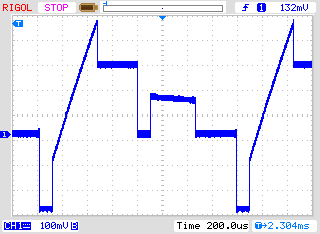
\includegraphics[width=9cm]{../PNG/ESR_4uF.png}
    \caption{Ein Pin gegen GND gemessen}
  \end{subfigure}
  ~
  \begin{subfigure}[b]{9cm}
    \centering
    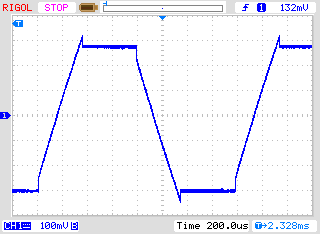
\includegraphics[width=9cm]{../PNG/ESR4uF6R8.png}
    \caption{Von Pin zu Pin gemessen}
  \end{subfigure}
  \caption{Spannungsverlauf eines \(4.2\mu F\) Kondensators während der ESR-Messung}
  \label{pic:esr4}
\end{figure}

\begin{figure}[H]
  \begin{subfigure}[b]{9cm}
    \centering
    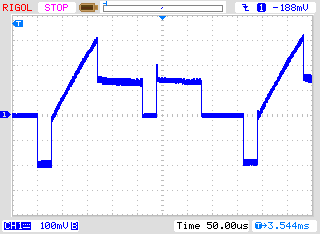
\includegraphics[width=9cm]{../PNG/ESR_2uF_pin2GND.png}
    \caption{Ein Pin gegen GND gemessen}
  \end{subfigure}
  ~
  \begin{subfigure}[b]{9cm}
    \centering
    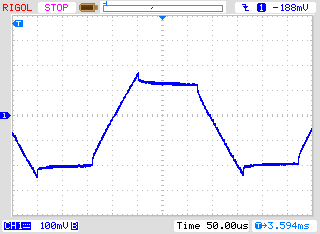
\includegraphics[width=9cm]{../PNG/ESR_2uF_pin2pin.png}
    \caption{Von Pin zu Pin gemessen}
  \end{subfigure}
  \caption{Spannungsverlauf eines \(2.2\mu F\) Kondensators während der ESR-Messung}
  \label{pic:esr2}
\end{figure}

Die Genauigkeit der ESR-Messung ist aus verschiedenen Gründen nicht sehr hoch:
\begin{enumerate}
\item Die Spannungsmessung an den beiden Kondensator-Anschlüssen kann nicht gleichzeitig sondern nur nacheinander durchgeführt werden.
 In der Zwischenzeit hat sich der Ladestrom durch den Ladevorgang des Kondensators geändert.
Dies wird versucht mit einer kapazitätsabhängigen Korrektur der Minuspol-Spannung auszugleichen.
\item Der ADC nimmt den Spannungswert 1,5 Takte nach dem Start des Wandlungsvorgangs. Der Wandelvorgang beginnt mit
der steigenden Flanke des ADC-Taktes, wenn das Startbit gesetzt ist. Wenn der Ladestrom des Kondensators zu früh abgeschaltet wird,
nimmt der ADC die falsche Spannung für die strombehaftete Messung auf. Wird der Ladestrom zu spät abgeschaltet, wird
der Kondensator weiter geladen als es der strombehafteten Messung entspricht.
Dann wird im stromlosen Zustand eine zu hohe Spannung gemessen.
Es ist aber schwierig im Programm den genauen Zeitpunkt für die Stromabschaltung zu treffen.
\item Der Port-Ausgangswiderstand wird bei dieser Messmethode als Referenz benutzt, dessen Widerstandwert
ist aber auch nicht exakt bekannt.
\item Die Auflösung des ADC reicht nicht aus, um eine Widerstandsauflösung von \(0.01 \Omega\) zu erreichen.
Für alle Messungen wird die interne Spannungsreferenz (1.1 V) benutzt, um die best mögliche Auflösung zu verwenden.
Zusätzlich wird versucht, den Auflösungs-Mangel durch eine große Zahl von Einzelmessungen abzumildern.
\item Mit der Abfrage des Fertig-Signals der ADC-Wandlung gelingt es nicht exakt, die Schaltzeiten der Port-Ausgänge mit dem
ADC-Takt zu synchronisieren.
\end{enumerate}

Trotz allen Schwierigkeiten scheinen die Ergebnisse brauchbar zu sein, wie die nachfolgende Abbildung \ref{fig:Cesr} zeigt.
Die ESR-Werte eines Bauteils gemessen mit dem Transistortester schwanken stärker als die Messungen des LCR-meters.
Die Messergebnisse des LCR-Messgerätes wurden bei einer Frequenz von 1 kHz gemessen oder für kleine Kapazitäten auf
2.4 kHz interpoliert.
Beim Transistortester muss auf die Qualität der Anschlüsse geachtet werden. Verwendete Anschlusskabel
erhöhen den gemessenen Widerstandswert. Auch die Kontakte von Steckverbindern können die gemessenen
Widerstandwerte erhöhen. Das LCR-Messgerät macht hier wegen den verwendeten Kelvin-Klemmen weniger Probleme.
Bei den Kondensatoren mit einer Kapazität unter \(1 \mu F\) war ein \(500 nF\) keramischer 
Kondensator (Z5U), alle anderen waren Folien-Kondensatoren. Der einzige Elektrolyt-Kondensator der Meßreihe unter \(9 \mu F\)  
ist ein \(2.2 \mu F\) Kondensator.

\begin{figure}[H]
\centering
% GNUPLOT: LaTeX picture with Postscript
\begingroup
  \makeatletter
  \providecommand\color[2][]{%
    \GenericError{(gnuplot) \space\space\space\@spaces}{%
      Package color not loaded in conjunction with
      terminal option `colourtext'%
    }{See the gnuplot documentation for explanation.%
    }{Either use 'blacktext' in gnuplot or load the package
      color.sty in LaTeX.}%
    \renewcommand\color[2][]{}%
  }%
  \providecommand\includegraphics[2][]{%
    \GenericError{(gnuplot) \space\space\space\@spaces}{%
      Package graphicx or graphics not loaded%
    }{See the gnuplot documentation for explanation.%
    }{The gnuplot epslatex terminal needs graphicx.sty or graphics.sty.}%
    \renewcommand\includegraphics[2][]{}%
  }%
  \providecommand\rotatebox[2]{#2}%
  \@ifundefined{ifGPcolor}{%
    \newif\ifGPcolor
    \GPcolortrue
  }{}%
  \@ifundefined{ifGPblacktext}{%
    \newif\ifGPblacktext
    \GPblacktexttrue
  }{}%
  % define a \g@addto@macro without @ in the name:
  \let\gplgaddtomacro\g@addto@macro
  % define empty templates for all commands taking text:
  \gdef\gplbacktext{}%
  \gdef\gplfronttext{}%
  \makeatother
  \ifGPblacktext
    % no textcolor at all
    \def\colorrgb#1{}%
    \def\colorgray#1{}%
  \else
    % gray or color?
    \ifGPcolor
      \def\colorrgb#1{\color[rgb]{#1}}%
      \def\colorgray#1{\color[gray]{#1}}%
      \expandafter\def\csname LTw\endcsname{\color{white}}%
      \expandafter\def\csname LTb\endcsname{\color{black}}%
      \expandafter\def\csname LTa\endcsname{\color{black}}%
      \expandafter\def\csname LT0\endcsname{\color[rgb]{1,0,0}}%
      \expandafter\def\csname LT1\endcsname{\color[rgb]{0,1,0}}%
      \expandafter\def\csname LT2\endcsname{\color[rgb]{0,0,1}}%
      \expandafter\def\csname LT3\endcsname{\color[rgb]{1,0,1}}%
      \expandafter\def\csname LT4\endcsname{\color[rgb]{0,1,1}}%
      \expandafter\def\csname LT5\endcsname{\color[rgb]{1,1,0}}%
      \expandafter\def\csname LT6\endcsname{\color[rgb]{0,0,0}}%
      \expandafter\def\csname LT7\endcsname{\color[rgb]{1,0.3,0}}%
      \expandafter\def\csname LT8\endcsname{\color[rgb]{0.5,0.5,0.5}}%
    \else
      % gray
      \def\colorrgb#1{\color{black}}%
      \def\colorgray#1{\color[gray]{#1}}%
      \expandafter\def\csname LTw\endcsname{\color{white}}%
      \expandafter\def\csname LTb\endcsname{\color{black}}%
      \expandafter\def\csname LTa\endcsname{\color{black}}%
      \expandafter\def\csname LT0\endcsname{\color{black}}%
      \expandafter\def\csname LT1\endcsname{\color{black}}%
      \expandafter\def\csname LT2\endcsname{\color{black}}%
      \expandafter\def\csname LT3\endcsname{\color{black}}%
      \expandafter\def\csname LT4\endcsname{\color{black}}%
      \expandafter\def\csname LT5\endcsname{\color{black}}%
      \expandafter\def\csname LT6\endcsname{\color{black}}%
      \expandafter\def\csname LT7\endcsname{\color{black}}%
      \expandafter\def\csname LT8\endcsname{\color{black}}%
    \fi
  \fi
  \setlength{\unitlength}{0.0500bp}%
  \begin{picture}(7200.00,5040.00)%
    \gplgaddtomacro\gplbacktext{%
      \csname LTb\endcsname%
      \put(946,704){\makebox(0,0)[r]{\strut{} 0}}%
      \csname LTb\endcsname%
      \put(946,1383){\makebox(0,0)[r]{\strut{} 0.2}}%
      \csname LTb\endcsname%
      \put(946,2061){\makebox(0,0)[r]{\strut{} 0.4}}%
      \csname LTb\endcsname%
      \put(946,2740){\makebox(0,0)[r]{\strut{} 0.6}}%
      \csname LTb\endcsname%
      \put(946,3418){\makebox(0,0)[r]{\strut{} 0.8}}%
      \csname LTb\endcsname%
      \put(946,4097){\makebox(0,0)[r]{\strut{} 1}}%
      \csname LTb\endcsname%
      \put(946,4775){\makebox(0,0)[r]{\strut{} 1.2}}%
      \csname LTb\endcsname%
      \put(1078,484){\makebox(0,0){\strut{}1u}}%
      \csname LTb\endcsname%
      \put(2986,484){\makebox(0,0){\strut{}10u}}%
      \csname LTb\endcsname%
      \put(4895,484){\makebox(0,0){\strut{}100u}}%
      \csname LTb\endcsname%
      \put(6803,484){\makebox(0,0){\strut{}1m}}%
      \put(176,2739){\rotatebox{-270}{\makebox(0,0){\strut{}ESR / Ohm}}}%
      \put(3940,154){\makebox(0,0){\strut{}Capacity value / F}}%
      \put(3940,4665){\makebox(0,0){\strut{}}}%
    }%
    \gplgaddtomacro\gplfronttext{%
      \csname LTb\endcsname%
      \put(5690,4594){\makebox(0,0)[r]{\strut{}328p}}%
      \csname LTb\endcsname%
      \put(5690,4358){\makebox(0,0)[r]{\strut{}328}}%
      \csname LTb\endcsname%
      \put(5690,4122){\makebox(0,0)[r]{\strut{}168p}}%
      \csname LTb\endcsname%
      \put(5690,3886){\makebox(0,0)[r]{\strut{}168a}}%
      \csname LTb\endcsname%
      \put(5690,3650){\makebox(0,0)[r]{\strut{}168}}%
      \csname LTb\endcsname%
      \put(5690,3414){\makebox(0,0)[r]{\strut{}LCR}}%
    }%
    \gplbacktext
    \put(0,0){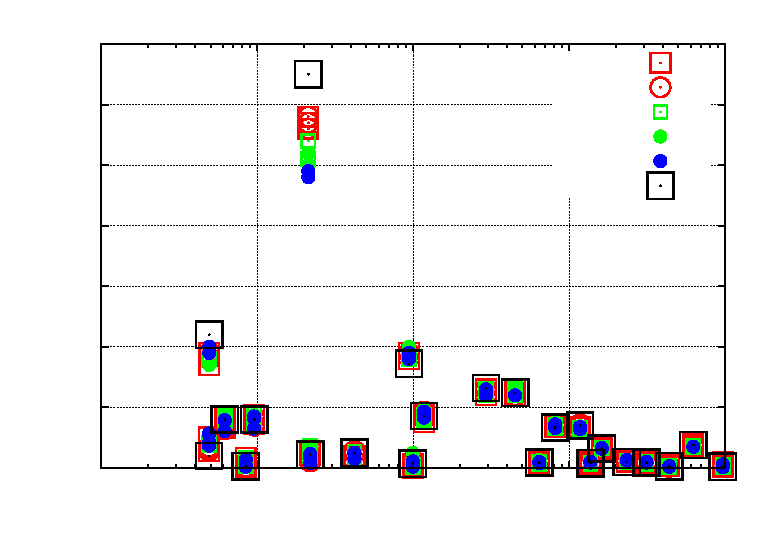
\includegraphics{../GNU/Cesr}}%
    \gplfronttext
  \end{picture}%
\endgroup

\caption{Messergebnisse der ESR-Messungen mit 15 veschiedenen ATmega}
\label{fig:Cesr}
\end{figure}

\newpage
\subsection{Messen des äquivalenten Serienwiderstandes ESR, Methode 2}
\label{sec:ESR2}
Ab der Softwareversion 1.07k wurde die ESR-Messung auf eine modifizierte Meßmethode umgestellt.
Die einzelnen Meßschritte sind in Abbildung~\ref{fig:Cap_esr2} gezeigt. Das besondere an der Methode
ist, daß die Zeit des Stromflusses durch den Kondensator wesentlich gegenüber der Methode 1 verringert wurde.
Der Kondensator wird mit einem Puls der halben Breite negativ vorgeladen und wird dann zyklisch aufgeladen und in der
Gegenrichtung wieder entladen.
Dabei wird der Ladepuls zeitlich so gelegt, daß bei Sample 4 und 8 zur Pulsmitte
die Spannung für den ADC abgegriffen wird (Sample and Hold, 2.5 ADC Takte nach dem Start).
Ein kompletter Meßzyklus wird in Abbildung~\ref{fig:Cap_esr2_timing} gezeigt.
Es werden auch bei dieser Meßmethode die Summen der Meßergebnisse aus 255 Zyklen ausgewertet,
um eine ausreichende Auflösung zu erreichen.
Eine fortlaufende Aufladung des Kondensators in die eine oder andere Richtung wird durch die kurzen und
gleich langen Auflade- und Entlade-Pulse bei gleicher Beschaltung weitgehend vermieden.
Bei der Messung der Referenzspannung fließt kein Strom durch den Kondensator. Dadurch ist diese Messung
nicht zeitkritisch. Es wird lediglich vorausgesetzt, daß der Kondensator seine Spannung in der
stromlosen Zeit beibehält.

\begin{figure}[H]
  \centering
    
\includegraphics[width=18cm]{../FIG/Cap_esr2_timing.eps}
  \caption{Zeitlicher Ablauf eines Meßzyklus der neuen ESR-Messung}
  \label{fig:Cap_esr2_timing}
\end{figure}

\begin{figure}[H]
  \centering
    
\includegraphics[]{../FIG/Cap_esr2.eps}
  \caption{Vereinfachte ESR-Messung eines Kondensators}
  \label{fig:Cap_esr2}
\end{figure}


Durch den kürzeren Ladepuls kann nicht nur der ESR von geringeren Kapazitätswerten gemessen werden, sondern
diese Methode kann auch für die Messung kleiner Widerstandswerte benutzt werden, wenn die Widerstände
keine meßbare Induktivität besitzen. Dadurch kann die Auflösung bei Widerstandswerten unter \(10 \Omega\) auf 
\(0.01 \Omega\) gesenkt werden. Daneben kann auch der Nullwiderstand für die Widerstandsmessung als auch
für die ESR-Messung im Selbsttestzweig der Kalibration für alle drei Testpin-Kombinationen bestimmt werden.
Auf solide Steckverbindungen oder Klemmverbindungen sollte für stabile Ergebnisse geachtet werden.
Die Meßperiode beträgt etwa \(900 \mu s\), was einer Frequenz von etwa \(1.1 kHz\) entspricht.
Wegen der Kürze der Ladepulse entspricht das Ergebnis aber eher einer Messung mit \(10 kHz\).
Als Beispiel wird die Messung eines \(10 \mu F\) Folienkondensators einmal direkt und einmal mit einem
\(2.7 \Omega\) Serienwiderstand in Abbildung~\ref{pic:NewEsr10} gezeigt.
Deutlich kann man den Einfluß des zusätzlichen Widerstandes beim Vergleich der beiden Diagramme erkennen.
Hier wird auch verständlich, warum die ADC-Messung in der Mitte des Ladepulses erfolgen muß.
Bei großen Kondensatoren bleibt der Ladestrom des Kondensators hinreichend gut konstant,
so daß bei der zeitlichen Mitte des Ladepulses auch die mittlere Spannung gemessen wird.
Bei keineren Kondensatoren ergibt sich ein deutlicherer Unterschied, der aber mit dem
bekannten Kapazitätswert relativ gut kompensiert werden kann.

\begin{figure}[H]
  \begin{subfigure}[b]{9cm}
    \centering
    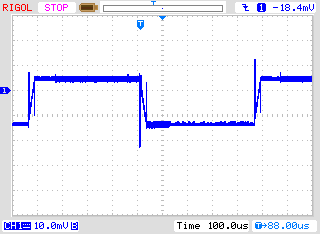
\includegraphics[width=9cm]{../PNG/NewEsr10uF0R0.png}
    \caption{ohne Serienwiderstand}
  \end{subfigure}
  ~
  \begin{subfigure}[b]{9cm}
    \centering
    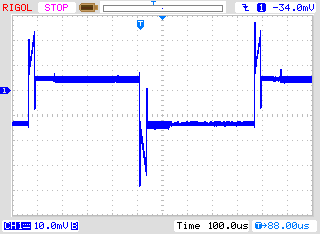
\includegraphics[width=9cm]{../PNG/NewEsr10uF2R7.png}
    \caption{mit \(2.7\Omega\) Serienwiderstand}
  \end{subfigure}
  \caption{Spannungsverlauf eines \(10\mu F\) Kondensators während der neuen ESR-Messung}
  \label{pic:NewEsr10}
\end{figure}

Die Meßergebnisse der neuen ESR-Meßmethode sind in Abbildung~\ref{fig:Cesr2} dargestellt.
Die ESR-Werte unterscheiden sich wegen der Frequenzabhängigkeit von den Ergebnissen der Abbildung~\ref{fig:Cesr}.
Die Vergleichswerte des LCR-Meßgerätes sind bei \(10 kHz\) ermittelt worden.

\begin{figure}[H]
\centering
% GNUPLOT: LaTeX picture with Postscript
\begingroup
  \makeatletter
  \providecommand\color[2][]{%
    \GenericError{(gnuplot) \space\space\space\@spaces}{%
      Package color not loaded in conjunction with
      terminal option `colourtext'%
    }{See the gnuplot documentation for explanation.%
    }{Either use 'blacktext' in gnuplot or load the package
      color.sty in LaTeX.}%
    \renewcommand\color[2][]{}%
  }%
  \providecommand\includegraphics[2][]{%
    \GenericError{(gnuplot) \space\space\space\@spaces}{%
      Package graphicx or graphics not loaded%
    }{See the gnuplot documentation for explanation.%
    }{The gnuplot epslatex terminal needs graphicx.sty or graphics.sty.}%
    \renewcommand\includegraphics[2][]{}%
  }%
  \providecommand\rotatebox[2]{#2}%
  \@ifundefined{ifGPcolor}{%
    \newif\ifGPcolor
    \GPcolortrue
  }{}%
  \@ifundefined{ifGPblacktext}{%
    \newif\ifGPblacktext
    \GPblacktexttrue
  }{}%
  % define a \g@addto@macro without @ in the name:
  \let\gplgaddtomacro\g@addto@macro
  % define empty templates for all commands taking text:
  \gdef\gplbacktext{}%
  \gdef\gplfronttext{}%
  \makeatother
  \ifGPblacktext
    % no textcolor at all
    \def\colorrgb#1{}%
    \def\colorgray#1{}%
  \else
    % gray or color?
    \ifGPcolor
      \def\colorrgb#1{\color[rgb]{#1}}%
      \def\colorgray#1{\color[gray]{#1}}%
      \expandafter\def\csname LTw\endcsname{\color{white}}%
      \expandafter\def\csname LTb\endcsname{\color{black}}%
      \expandafter\def\csname LTa\endcsname{\color{black}}%
      \expandafter\def\csname LT0\endcsname{\color[rgb]{1,0,0}}%
      \expandafter\def\csname LT1\endcsname{\color[rgb]{0,1,0}}%
      \expandafter\def\csname LT2\endcsname{\color[rgb]{0,0,1}}%
      \expandafter\def\csname LT3\endcsname{\color[rgb]{1,0,1}}%
      \expandafter\def\csname LT4\endcsname{\color[rgb]{0,1,1}}%
      \expandafter\def\csname LT5\endcsname{\color[rgb]{1,1,0}}%
      \expandafter\def\csname LT6\endcsname{\color[rgb]{0,0,0}}%
      \expandafter\def\csname LT7\endcsname{\color[rgb]{1,0.3,0}}%
      \expandafter\def\csname LT8\endcsname{\color[rgb]{0.5,0.5,0.5}}%
    \else
      % gray
      \def\colorrgb#1{\color{black}}%
      \def\colorgray#1{\color[gray]{#1}}%
      \expandafter\def\csname LTw\endcsname{\color{white}}%
      \expandafter\def\csname LTb\endcsname{\color{black}}%
      \expandafter\def\csname LTa\endcsname{\color{black}}%
      \expandafter\def\csname LT0\endcsname{\color{black}}%
      \expandafter\def\csname LT1\endcsname{\color{black}}%
      \expandafter\def\csname LT2\endcsname{\color{black}}%
      \expandafter\def\csname LT3\endcsname{\color{black}}%
      \expandafter\def\csname LT4\endcsname{\color{black}}%
      \expandafter\def\csname LT5\endcsname{\color{black}}%
      \expandafter\def\csname LT6\endcsname{\color{black}}%
      \expandafter\def\csname LT7\endcsname{\color{black}}%
      \expandafter\def\csname LT8\endcsname{\color{black}}%
    \fi
  \fi
  \setlength{\unitlength}{0.0500bp}%
  \begin{picture}(7200.00,5040.00)%
    \gplgaddtomacro\gplbacktext{%
      \csname LTb\endcsname%
      \put(1078,704){\makebox(0,0)[r]{\strut{} 0.01}}%
      \csname LTb\endcsname%
      \put(1078,2061){\makebox(0,0)[r]{\strut{} 0.1}}%
      \csname LTb\endcsname%
      \put(1078,3418){\makebox(0,0)[r]{\strut{} 1}}%
      \csname LTb\endcsname%
      \put(1078,4775){\makebox(0,0)[r]{\strut{} 10}}%
      \csname LTb\endcsname%
      \put(1210,484){\makebox(0,0){\strut{}100n}}%
      \csname LTb\endcsname%
      \put(2608,484){\makebox(0,0){\strut{}1u}}%
      \csname LTb\endcsname%
      \put(4007,484){\makebox(0,0){\strut{}10u}}%
      \csname LTb\endcsname%
      \put(5405,484){\makebox(0,0){\strut{}100u}}%
      \csname LTb\endcsname%
      \put(6803,484){\makebox(0,0){\strut{}1m}}%
      \put(176,2739){\rotatebox{-270}{\makebox(0,0){\strut{}ESR / Ohm}}}%
      \put(4006,154){\makebox(0,0){\strut{}Capacity value / F}}%
      \put(4006,4665){\makebox(0,0){\strut{}}}%
    }%
    \gplgaddtomacro\gplfronttext{%
      \csname LTb\endcsname%
      \put(5690,4594){\makebox(0,0)[r]{\strut{}328p}}%
      \csname LTb\endcsname%
      \put(5690,4358){\makebox(0,0)[r]{\strut{}328}}%
      \csname LTb\endcsname%
      \put(5690,4122){\makebox(0,0)[r]{\strut{}168p}}%
      \csname LTb\endcsname%
      \put(5690,3886){\makebox(0,0)[r]{\strut{}168a}}%
      \csname LTb\endcsname%
      \put(5690,3650){\makebox(0,0)[r]{\strut{}168}}%
      \csname LTb\endcsname%
      \put(5690,3414){\makebox(0,0)[r]{\strut{}LCR}}%
    }%
    \gplbacktext
    \put(0,0){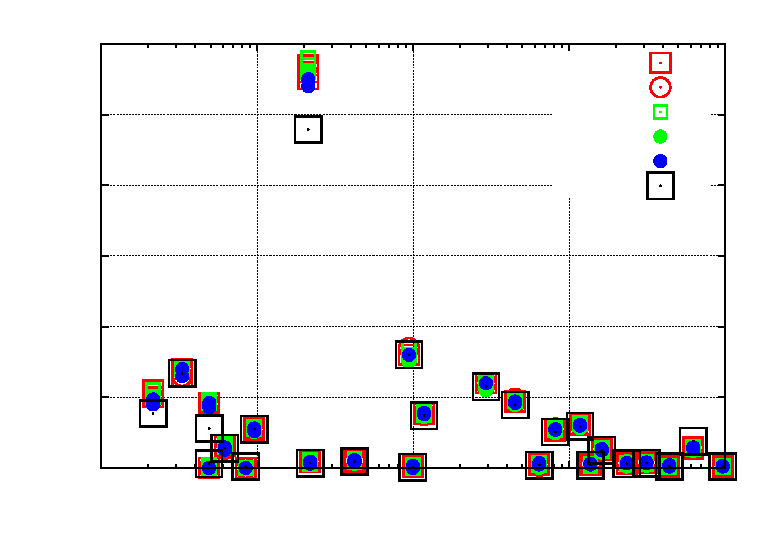
\includegraphics{../GNU/Cesr2}}%
    \gplfronttext
  \end{picture}%
\endgroup

\caption{Messergebnisse der ESR-Messungen mit 15 veschiedenen ATmega, Methode 2}
\label{fig:Cesr2}
\end{figure}

Eine Meßreihe mit Elektrolyt-Kondensatoren verschiedener Größen zeigt die Abbildung \ref{fig:ElcoESR}.
Es werden die Ergebnisse von einem PeakTech 3315 LCR-Meßgerät bei verschiedenen Meßfrequenzen und die
Ergebnisse des TransistorTesters gegenübergestellt. Die Widerstandswerte sind in diesem Diagram lograrithmisch dargestellt.
In allen Fällen liegen die Ergebnisse des TransistorTesters
nahe an den Ergebnissen des LCR-Meßgerätes bei 10kHz Meßfrequenz. 
Nur der \(500 \mu F/3V\) Kondensator war ein älteres Exemplar, alle anderen waren neuwertig.

\begin{figure}[H]
\centering
% GNUPLOT: LaTeX picture with Postscript
\begingroup
  \makeatletter
  \providecommand\color[2][]{%
    \GenericError{(gnuplot) \space\space\space\@spaces}{%
      Package color not loaded in conjunction with
      terminal option `colourtext'%
    }{See the gnuplot documentation for explanation.%
    }{Either use 'blacktext' in gnuplot or load the package
      color.sty in LaTeX.}%
    \renewcommand\color[2][]{}%
  }%
  \providecommand\includegraphics[2][]{%
    \GenericError{(gnuplot) \space\space\space\@spaces}{%
      Package graphicx or graphics not loaded%
    }{See the gnuplot documentation for explanation.%
    }{The gnuplot epslatex terminal needs graphicx.sty or graphics.sty.}%
    \renewcommand\includegraphics[2][]{}%
  }%
  \providecommand\rotatebox[2]{#2}%
  \@ifundefined{ifGPcolor}{%
    \newif\ifGPcolor
    \GPcolortrue
  }{}%
  \@ifundefined{ifGPblacktext}{%
    \newif\ifGPblacktext
    \GPblacktexttrue
  }{}%
  % define a \g@addto@macro without @ in the name:
  \let\gplgaddtomacro\g@addto@macro
  % define empty templates for all commands taking text:
  \gdef\gplbacktext{}%
  \gdef\gplfronttext{}%
  \makeatother
  \ifGPblacktext
    % no textcolor at all
    \def\colorrgb#1{}%
    \def\colorgray#1{}%
  \else
    % gray or color?
    \ifGPcolor
      \def\colorrgb#1{\color[rgb]{#1}}%
      \def\colorgray#1{\color[gray]{#1}}%
      \expandafter\def\csname LTw\endcsname{\color{white}}%
      \expandafter\def\csname LTb\endcsname{\color{black}}%
      \expandafter\def\csname LTa\endcsname{\color{black}}%
      \expandafter\def\csname LT0\endcsname{\color[rgb]{1,0,0}}%
      \expandafter\def\csname LT1\endcsname{\color[rgb]{0,1,0}}%
      \expandafter\def\csname LT2\endcsname{\color[rgb]{0,0,1}}%
      \expandafter\def\csname LT3\endcsname{\color[rgb]{1,0,1}}%
      \expandafter\def\csname LT4\endcsname{\color[rgb]{0,1,1}}%
      \expandafter\def\csname LT5\endcsname{\color[rgb]{1,1,0}}%
      \expandafter\def\csname LT6\endcsname{\color[rgb]{0,0,0}}%
      \expandafter\def\csname LT7\endcsname{\color[rgb]{1,0.3,0}}%
      \expandafter\def\csname LT8\endcsname{\color[rgb]{0.5,0.5,0.5}}%
    \else
      % gray
      \def\colorrgb#1{\color{black}}%
      \def\colorgray#1{\color[gray]{#1}}%
      \expandafter\def\csname LTw\endcsname{\color{white}}%
      \expandafter\def\csname LTb\endcsname{\color{black}}%
      \expandafter\def\csname LTa\endcsname{\color{black}}%
      \expandafter\def\csname LT0\endcsname{\color{black}}%
      \expandafter\def\csname LT1\endcsname{\color{black}}%
      \expandafter\def\csname LT2\endcsname{\color{black}}%
      \expandafter\def\csname LT3\endcsname{\color{black}}%
      \expandafter\def\csname LT4\endcsname{\color{black}}%
      \expandafter\def\csname LT5\endcsname{\color{black}}%
      \expandafter\def\csname LT6\endcsname{\color{black}}%
      \expandafter\def\csname LT7\endcsname{\color{black}}%
      \expandafter\def\csname LT8\endcsname{\color{black}}%
    \fi
  \fi
  \setlength{\unitlength}{0.0500bp}%
  \begin{picture}(7200.00,5040.00)%
    \gplgaddtomacro\gplbacktext{%
      \csname LTb\endcsname%
      \put(1078,1540){\makebox(0,0)[r]{\strut{} 0.01}}%
      \csname LTb\endcsname%
      \put(1078,2349){\makebox(0,0)[r]{\strut{} 0.1}}%
      \csname LTb\endcsname%
      \put(1078,3158){\makebox(0,0)[r]{\strut{} 1}}%
      \csname LTb\endcsname%
      \put(1078,3966){\makebox(0,0)[r]{\strut{} 10}}%
      \csname LTb\endcsname%
      \put(1078,4775){\makebox(0,0)[r]{\strut{} 100}}%
      \csname LTb\endcsname%
      \put(1521,1408){\rotatebox{-270}{\makebox(0,0)[r]{\strut{}0.47u/100V}}}%
      \csname LTb\endcsname%
      \put(1831,1408){\rotatebox{-270}{\makebox(0,0)[r]{\strut{}1u/100V}}}%
      \csname LTb\endcsname%
      \put(2142,1408){\rotatebox{-270}{\makebox(0,0)[r]{\strut{}1u/50V}}}%
      \csname LTb\endcsname%
      \put(2453,1408){\rotatebox{-270}{\makebox(0,0)[r]{\strut{}2.2u/100V}}}%
      \csname LTb\endcsname%
      \put(2764,1408){\rotatebox{-270}{\makebox(0,0)[r]{\strut{}2.2u/50V}}}%
      \csname LTb\endcsname%
      \put(3074,1408){\rotatebox{-270}{\makebox(0,0)[r]{\strut{}3.3u/100V}}}%
      \csname LTb\endcsname%
      \put(3385,1408){\rotatebox{-270}{\makebox(0,0)[r]{\strut{}4.7u/63V}}}%
      \csname LTb\endcsname%
      \put(3696,1408){\rotatebox{-270}{\makebox(0,0)[r]{\strut{}4.7u/50V}}}%
      \csname LTb\endcsname%
      \put(4007,1408){\rotatebox{-270}{\makebox(0,0)[r]{\strut{}10u/50V}}}%
      \csname LTb\endcsname%
      \put(4317,1408){\rotatebox{-270}{\makebox(0,0)[r]{\strut{}22u/10V}}}%
      \csname LTb\endcsname%
      \put(4628,1408){\rotatebox{-270}{\makebox(0,0)[r]{\strut{}22u/63V}}}%
      \csname LTb\endcsname%
      \put(4939,1408){\rotatebox{-270}{\makebox(0,0)[r]{\strut{}33u/63V}}}%
      \csname LTb\endcsname%
      \put(5249,1408){\rotatebox{-270}{\makebox(0,0)[r]{\strut{}47u/63V}}}%
      \csname LTb\endcsname%
      \put(5560,1408){\rotatebox{-270}{\makebox(0,0)[r]{\strut{}100u/63V}}}%
      \csname LTb\endcsname%
      \put(5871,1408){\rotatebox{-270}{\makebox(0,0)[r]{\strut{}220u/63V}}}%
      \csname LTb\endcsname%
      \put(6182,1408){\rotatebox{-270}{\makebox(0,0)[r]{\strut{}470u/35V}}}%
      \csname LTb\endcsname%
      \put(6492,1408){\rotatebox{-270}{\makebox(0,0)[r]{\strut{}500u/3V}}}%
      \put(176,3157){\rotatebox{-270}{\makebox(0,0){\strut{}ESR / Ohm}}}%
      \put(4006,-66){\makebox(0,0){\strut{}}}%
      \put(4006,4665){\makebox(0,0){\strut{}}}%
    }%
    \gplgaddtomacro\gplfronttext{%
      \csname LTb\endcsname%
      \put(5816,4602){\makebox(0,0)[r]{\strut{}LCR-100Hz}}%
      \csname LTb\endcsname%
      \put(5816,4382){\makebox(0,0)[r]{\strut{}LCR-1kHz}}%
      \csname LTb\endcsname%
      \put(5816,4162){\makebox(0,0)[r]{\strut{}LCR-10kHz}}%
      \csname LTb\endcsname%
      \put(5816,3942){\makebox(0,0)[r]{\strut{}LCR-100kHz}}%
      \csname LTb\endcsname%
      \put(5816,3722){\makebox(0,0)[r]{\strut{}TTester}}%
    }%
    \gplbacktext
    \put(0,0){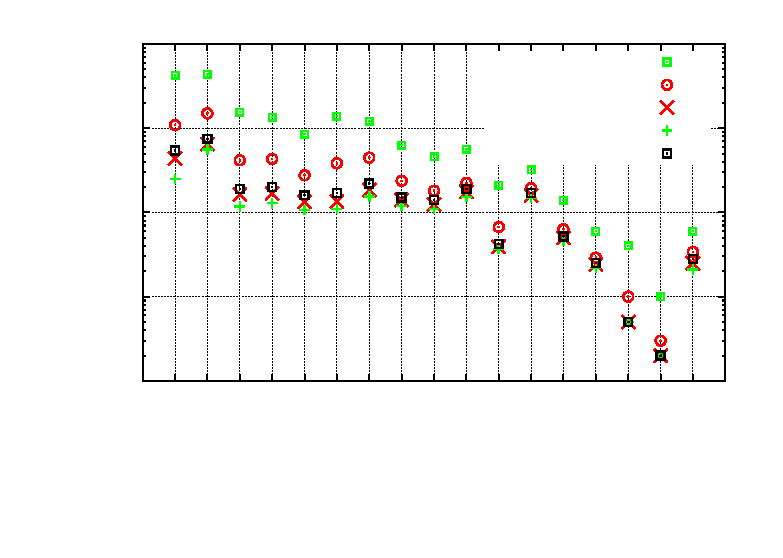
\includegraphics{../GNU/Elco_esr}}%
    \gplfronttext
  \end{picture}%
\endgroup

\caption{Ergebnisse der ESR-Messungen von verschiedenen Elektrolyt-Kondensatoren}
\label{fig:ElcoESR}
\end{figure}

Da mit der neuen Methode auch Widerstände gemessen werden können, werden in Abbildung~\ref{fig:res_esr} die
Meßfehler der Messung von einigen Widerständen unter \(10 \Omega\) mit jeweils drei Exemplaren verschiedener
ATmega gezeigt.  

\begin{figure}[H]
\centering
% GNUPLOT: LaTeX picture with Postscript
\begingroup
  \makeatletter
  \providecommand\color[2][]{%
    \GenericError{(gnuplot) \space\space\space\@spaces}{%
      Package color not loaded in conjunction with
      terminal option `colourtext'%
    }{See the gnuplot documentation for explanation.%
    }{Either use 'blacktext' in gnuplot or load the package
      color.sty in LaTeX.}%
    \renewcommand\color[2][]{}%
  }%
  \providecommand\includegraphics[2][]{%
    \GenericError{(gnuplot) \space\space\space\@spaces}{%
      Package graphicx or graphics not loaded%
    }{See the gnuplot documentation for explanation.%
    }{The gnuplot epslatex terminal needs graphicx.sty or graphics.sty.}%
    \renewcommand\includegraphics[2][]{}%
  }%
  \providecommand\rotatebox[2]{#2}%
  \@ifundefined{ifGPcolor}{%
    \newif\ifGPcolor
    \GPcolortrue
  }{}%
  \@ifundefined{ifGPblacktext}{%
    \newif\ifGPblacktext
    \GPblacktexttrue
  }{}%
  % define a \g@addto@macro without @ in the name:
  \let\gplgaddtomacro\g@addto@macro
  % define empty templates for all commands taking text:
  \gdef\gplbacktext{}%
  \gdef\gplfronttext{}%
  \makeatother
  \ifGPblacktext
    % no textcolor at all
    \def\colorrgb#1{}%
    \def\colorgray#1{}%
  \else
    % gray or color?
    \ifGPcolor
      \def\colorrgb#1{\color[rgb]{#1}}%
      \def\colorgray#1{\color[gray]{#1}}%
      \expandafter\def\csname LTw\endcsname{\color{white}}%
      \expandafter\def\csname LTb\endcsname{\color{black}}%
      \expandafter\def\csname LTa\endcsname{\color{black}}%
      \expandafter\def\csname LT0\endcsname{\color[rgb]{1,0,0}}%
      \expandafter\def\csname LT1\endcsname{\color[rgb]{0,1,0}}%
      \expandafter\def\csname LT2\endcsname{\color[rgb]{0,0,1}}%
      \expandafter\def\csname LT3\endcsname{\color[rgb]{1,0,1}}%
      \expandafter\def\csname LT4\endcsname{\color[rgb]{0,1,1}}%
      \expandafter\def\csname LT5\endcsname{\color[rgb]{1,1,0}}%
      \expandafter\def\csname LT6\endcsname{\color[rgb]{0,0,0}}%
      \expandafter\def\csname LT7\endcsname{\color[rgb]{1,0.3,0}}%
      \expandafter\def\csname LT8\endcsname{\color[rgb]{0.5,0.5,0.5}}%
    \else
      % gray
      \def\colorrgb#1{\color{black}}%
      \def\colorgray#1{\color[gray]{#1}}%
      \expandafter\def\csname LTw\endcsname{\color{white}}%
      \expandafter\def\csname LTb\endcsname{\color{black}}%
      \expandafter\def\csname LTa\endcsname{\color{black}}%
      \expandafter\def\csname LT0\endcsname{\color{black}}%
      \expandafter\def\csname LT1\endcsname{\color{black}}%
      \expandafter\def\csname LT2\endcsname{\color{black}}%
      \expandafter\def\csname LT3\endcsname{\color{black}}%
      \expandafter\def\csname LT4\endcsname{\color{black}}%
      \expandafter\def\csname LT5\endcsname{\color{black}}%
      \expandafter\def\csname LT6\endcsname{\color{black}}%
      \expandafter\def\csname LT7\endcsname{\color{black}}%
      \expandafter\def\csname LT8\endcsname{\color{black}}%
    \fi
  \fi
  \setlength{\unitlength}{0.0500bp}%
  \begin{picture}(7200.00,5040.00)%
    \gplgaddtomacro\gplbacktext{%
      \csname LTb\endcsname%
      \put(1078,704){\makebox(0,0)[r]{\strut{}-0.2}}%
      \csname LTb\endcsname%
      \put(1078,1213){\makebox(0,0)[r]{\strut{}-0.15}}%
      \csname LTb\endcsname%
      \put(1078,1722){\makebox(0,0)[r]{\strut{}-0.1}}%
      \csname LTb\endcsname%
      \put(1078,2231){\makebox(0,0)[r]{\strut{}-0.05}}%
      \csname LTb\endcsname%
      \put(1078,2740){\makebox(0,0)[r]{\strut{} 0}}%
      \csname LTb\endcsname%
      \put(1078,3248){\makebox(0,0)[r]{\strut{} 0.05}}%
      \csname LTb\endcsname%
      \put(1078,3757){\makebox(0,0)[r]{\strut{} 0.1}}%
      \csname LTb\endcsname%
      \put(1078,4266){\makebox(0,0)[r]{\strut{} 0.15}}%
      \csname LTb\endcsname%
      \put(1078,4775){\makebox(0,0)[r]{\strut{} 0.2}}%
      \csname LTb\endcsname%
      \put(1210,484){\makebox(0,0){\strut{} 0}}%
      \csname LTb\endcsname%
      \put(1956,484){\makebox(0,0){\strut{} 2}}%
      \csname LTb\endcsname%
      \put(2701,484){\makebox(0,0){\strut{} 4}}%
      \csname LTb\endcsname%
      \put(3447,484){\makebox(0,0){\strut{} 6}}%
      \csname LTb\endcsname%
      \put(4193,484){\makebox(0,0){\strut{} 8}}%
      \csname LTb\endcsname%
      \put(4939,484){\makebox(0,0){\strut{} 10}}%
      \csname LTb\endcsname%
      \put(5684,484){\makebox(0,0){\strut{} 12}}%
      \csname LTb\endcsname%
      \put(6430,484){\makebox(0,0){\strut{} 14}}%
      \put(176,2739){\rotatebox{-270}{\makebox(0,0){\strut{}difference / Ohm}}}%
      \put(4006,154){\makebox(0,0){\strut{}Resistor value / Ohm}}%
    }%
    \gplgaddtomacro\gplfronttext{%
      \csname LTb\endcsname%
      \put(5753,4602){\makebox(0,0)[r]{\strut{}m168}}%
      \csname LTb\endcsname%
      \put(5753,4382){\makebox(0,0)[r]{\strut{}m168a}}%
      \csname LTb\endcsname%
      \put(5753,4162){\makebox(0,0)[r]{\strut{}m168p}}%
      \csname LTb\endcsname%
      \put(5753,3942){\makebox(0,0)[r]{\strut{}m328}}%
      \csname LTb\endcsname%
      \put(5753,3722){\makebox(0,0)[r]{\strut{}m328p}}%
    }%
    \gplbacktext
    \put(0,0){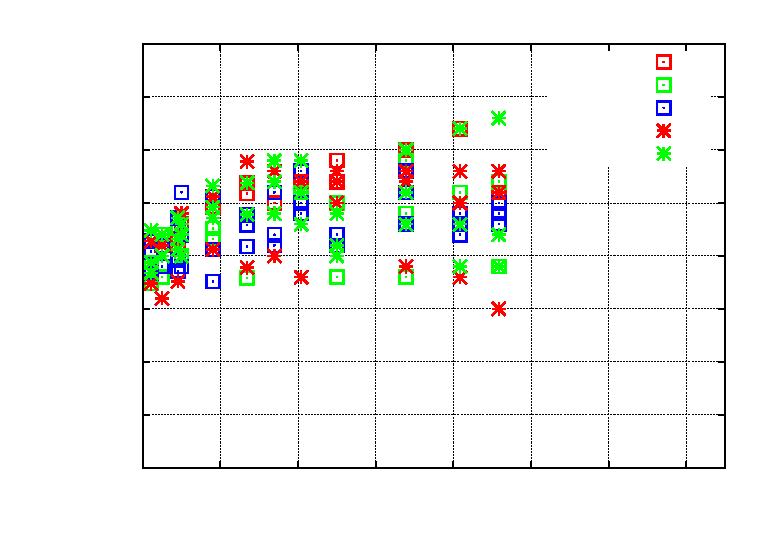
\includegraphics{../GNU/res_esr}}%
    \gplfronttext
  \end{picture}%
\endgroup

\caption{Messfehler von Widerständen mit der ESR Messung}
\label{fig:res_esr}
\end{figure}


\subsection{Spannungsverlust nach einem Ladepuls, Vloss}
Beim Meßverfahren von großen Kapazitäten wird der Spannungsverlust nach einem Ladepuls im stromlosen Zustand untersucht.
Die erreichte Ladespannung sinkt bei Elektrolyt-Kondensatoren nach kurzer Zeit wieder etwas ab.
Dieser Spannungsverlust kann durch einen parallel geschalteten Widerstand verursacht werden.
Ich nehme an, daß der Spannungsverlust bei Elektrolyt-Kondensatoren durch eine interne Ladungsverteilung nach
dem Ladepuls verursacht wird. Bei einem langsamen Ladevorgang, wie er bei kleineren Kapazitäten mit dem \(470 k\Omega\) Widerstand
gemacht wird, ist diese Umverteilung schon während des Ladevorgangs abgeschlossen. Dann tritt kein meßbarer Spannungsverlust nach
der Ladung in der betrachteten Zeitspanne auf. Wird der gleiche Elektrolyt-Kondensator aber mit einem
kurzem pulsförmigen Strom geladen, ist hier auch ein Spannungsverlust durch die nachträgliche Umverteilung
der Ladung zu beobachten. Der gleiche Effekt ist in geringerem Umfang auch bei keramischen Kondensatoren zu beobachten. 
Nach den bisherigen Beobachtungen sind Kondensatoren mit mehreren \% Spannungsverlust verdächtig.
Besonders auffällig in Bezug auf den Spannungsverlust sind auch ältere Papierkondensatoren, die auch für andere Meßgeräte
eine Herausforderung sind. Dies will ich in folgender Tabelle verdeutlichen.
\vspace{0.5 cm}

\begin{tabular}{| l | c | c | c | c | c | c |}
   \hline
Kondensator & Nenn-      & PeakTech     & Voltcraft & PeakTech & Transistor- \\
Type        & Kapazität  & LCR 2170     & M2650-B   &  3315    & Tester      \\
    \hline
    \hline
Papier     & 4700pF      & 6.75-10.36nF & 8.00nF    &  25.40nF &  10.71nF   \\
           &             &  Q=2.5-32    &           &          &  Vloss=11 \% \\
    \hline
Papier     & 6800pF      & 9.40-11.40nF & 10.41nF   &  23.30nF &  11.65nF  \\
           &             &  Q=5-25      &           &          &  Vloss=5.0 \% \\
    \hline
unbekannt  & 4700pF      & 5.85-6.33nF  & 6.12nF    &  6.90nF  &  6225pF  \\
           &             &  Q=16-87     &           &          &  Vloss=1.7 \% \\
    \hline
Folie      & 7870pF      & 7.86-7.87nF  & 7.95nF    &  7.95nF  &  7872pF  \\
           &             &  Q= \textgreater~1540    &           &          &  Vloss=0 \% \\
    \hline
Papier     & 22000pF     & 37.4-57.5nF  & 52.8nF    &  112nF   &  118.5nF \\
           &             &  Q=2.5-32    &           &          &  Vloss=12 \% \\
    \hline
Folie      & 22600pF     & 22.4-22.5nF  & 22.57nF   & 22.69nF  &  22.54nF \\
           &             & Q= \textgreater~1540     &           &          &  Vloss=0 \% \\
    \hline
Papier     & 100nF       & 144-256nF    & 177nF     &  318nF   &  529.7nF \\
           &             & Q=2.6-28     &           &          &  Vloss=12 \% \\
    \hline
Keramisch  & 100nF       & 97.7-102nF   & 103.7nF   & 103.3nF  &  103.1nF \\
           &             & Q=90-134     &           &          &  Vloss=0.1 \% \\
    \hline
Folie      & 100nF       & 98.0-101nF   & 101.4nF   & 102.2nF  &  101.6nF \\
           &             & Q=58-700     &           &          &  Vloss=0 \% \\
    \hline
\end{tabular}
\vspace{0.5 cm}


In der Tabelle kann man sehen, daß die Kapazität aller Folienkondensatoren mit befriedigender Genauigkeit von allen
Meßgeräten bestimmt werden. Die Kapazitäten und die Güten Q des PeakTech LCR-Meßgerätes sind Minumum
und Maximum der Meßergebnisse im Frequenzbereich \(100 Hz\) bis \(100 kHz\).
Bei allen Beispielen in der Tabelle ist der Spannungsverlust Vloss des TransistorTesters groß,
wenn die Kondensatoren eine geringe Güte haben. Nur in diesem Fall sind auch große Abweichungen
der gemessenen Kapazität zu beobachten. Damit der Spannungsverlust eines Kondensators vom
Transistortester gemessen werden kann, muß die gemessene Kapazität größer als \(5000 pF\) sein.

\subsection{Separate Kapazitäts- und ESR-Messung}
Die separate Kapazitätsmessung mit anschließender ESR-Messung ist nur für ATmega mit genügend Speicher
über den Bediendialog wählbar. Diese Art der Messung ist dafür gedacht, Kondensatoren im eingelöteten
Zustand messen zu können. 
Bitte sorgen Sie dafür, daß alle Kondensatoren auf der Leiterplatte entladen sind, bevor Sie mit den
Messungen beginnen.
Um die Messung im eingebauten Zustand zu ermöglichen, wird dafür gesorgt,
daß die Meßspannung möglichst nur knapp über 300mV beträgt.
Außerdem wird für die Messung nur mit dem \(680 \Omega\) Widerstand durchgeführt um den Einfluß von
Restströmen der angeschlossenen Bauteilen auf der Leiterplatte gering zu halten.
Um möglichst kleine Kapazitätswerte messen zu können, wird mit einem nur \(200 \mu s\) kurzen Ladepuls
begonnen. Wenn die Ladespannung erwarten läßt, daß auch bei einem \(2 ms\) langen Ladepuls die Ladespannung
von \(300 mV\) nicht überschritten wird, wird danach \(2 ms\) lang weitergeladen. Wenn bei sehr großen
Kapazitätswerten auch dann noch kein deutlicher Spannungszuwachs festzustellen ist, wird sogar mit
\(20 ms\) langen Ladepulsen weitergeladen. Bei Annäherung der Spannung an die \(300 mV\) wird wieder
mit den kürzeren Ladepulsen weitergeladen. Die gesamte Ladezeit wird dabei zusammengezählt und nach
Überschreitung der \(300 mV\) die Kapazität aus der geladenen Spannung und der Ladezeit bestimmt.
Mit diesem Verfahren sind Kapazitätswerte von unter \(2 \mu F\) meßbar. Die Obergrenze der Kapazität
bei dieser Messung beträgt wegen einer Ladezeitbegrenzung auf \(2.5 s\) etwa \(50 mF\).
Wenn ein Kapazitätswert gemessen wurde, wird danach der ESR-Wert des Kondensators mit dem schon
im Kapitel~\ref{sec:ESR2} beschriebenen Verfahren gemessen.
Die Ergebnisse werden nur kurz angezeigt und danach sofort mit der nächsten Messung begonnen.
Die Meßserie wird nach 250 Messungen oder auf Tastendruck abgebrochen und dann zum Bedienmenü zurückgekehrt.

\subsection{Ergebnisse der Kondensator-Messung}
Die Ergebnisse meiner Messungen werden in Abbildung~\ref{fig:mega8cap} für drei ATmega8 dargestellt.
Zusätzlich sind einige Werte der Original-Software mit einem Korrekturfaktor
von 0,88~(-12\%) dargestellt.
Weitere Ergebnisse von ATmega8 Versionen zeigen die Abbildungen~\ref{fig:mega8Acap} und \ref{fig:mega8Lcap}.
Die Ergebnisse der Messung der gleichen Kondensatoren mit einem ATmega168 werden in Abbildung~\ref{fig:mega168cap} gezeigt.
Die Referenz für die Fehlerberechnung sind die Messwerte eines PeakTech 2170 LCR-Messgerätes, 
 nicht die aufgedruckten Werte der Bauteile.
Die grösseren relativen Messfehler bei großen Kondensatoren liegen zum Teil an der zu hohen Messfrequenz (100 Hz) des
LCR-Messgerätes für große Elektrolytkondensatoren, zum anderen spielt auch die schlechte Güte der
Elektrolytkondensatoren eine Rolle.

\begin{figure}[H]
\centering
% GNUPLOT: LaTeX picture with Postscript
\begingroup
  \makeatletter
  \providecommand\color[2][]{%
    \GenericError{(gnuplot) \space\space\space\@spaces}{%
      Package color not loaded in conjunction with
      terminal option `colourtext'%
    }{See the gnuplot documentation for explanation.%
    }{Either use 'blacktext' in gnuplot or load the package
      color.sty in LaTeX.}%
    \renewcommand\color[2][]{}%
  }%
  \providecommand\includegraphics[2][]{%
    \GenericError{(gnuplot) \space\space\space\@spaces}{%
      Package graphicx or graphics not loaded%
    }{See the gnuplot documentation for explanation.%
    }{The gnuplot epslatex terminal needs graphicx.sty or graphics.sty.}%
    \renewcommand\includegraphics[2][]{}%
  }%
  \providecommand\rotatebox[2]{#2}%
  \@ifundefined{ifGPcolor}{%
    \newif\ifGPcolor
    \GPcolortrue
  }{}%
  \@ifundefined{ifGPblacktext}{%
    \newif\ifGPblacktext
    \GPblacktexttrue
  }{}%
  % define a \g@addto@macro without @ in the name:
  \let\gplgaddtomacro\g@addto@macro
  % define empty templates for all commands taking text:
  \gdef\gplbacktext{}%
  \gdef\gplfronttext{}%
  \makeatother
  \ifGPblacktext
    % no textcolor at all
    \def\colorrgb#1{}%
    \def\colorgray#1{}%
  \else
    % gray or color?
    \ifGPcolor
      \def\colorrgb#1{\color[rgb]{#1}}%
      \def\colorgray#1{\color[gray]{#1}}%
      \expandafter\def\csname LTw\endcsname{\color{white}}%
      \expandafter\def\csname LTb\endcsname{\color{black}}%
      \expandafter\def\csname LTa\endcsname{\color{black}}%
      \expandafter\def\csname LT0\endcsname{\color[rgb]{1,0,0}}%
      \expandafter\def\csname LT1\endcsname{\color[rgb]{0,1,0}}%
      \expandafter\def\csname LT2\endcsname{\color[rgb]{0,0,1}}%
      \expandafter\def\csname LT3\endcsname{\color[rgb]{1,0,1}}%
      \expandafter\def\csname LT4\endcsname{\color[rgb]{0,1,1}}%
      \expandafter\def\csname LT5\endcsname{\color[rgb]{1,1,0}}%
      \expandafter\def\csname LT6\endcsname{\color[rgb]{0,0,0}}%
      \expandafter\def\csname LT7\endcsname{\color[rgb]{1,0.3,0}}%
      \expandafter\def\csname LT8\endcsname{\color[rgb]{0.5,0.5,0.5}}%
    \else
      % gray
      \def\colorrgb#1{\color{black}}%
      \def\colorgray#1{\color[gray]{#1}}%
      \expandafter\def\csname LTw\endcsname{\color{white}}%
      \expandafter\def\csname LTb\endcsname{\color{black}}%
      \expandafter\def\csname LTa\endcsname{\color{black}}%
      \expandafter\def\csname LT0\endcsname{\color{black}}%
      \expandafter\def\csname LT1\endcsname{\color{black}}%
      \expandafter\def\csname LT2\endcsname{\color{black}}%
      \expandafter\def\csname LT3\endcsname{\color{black}}%
      \expandafter\def\csname LT4\endcsname{\color{black}}%
      \expandafter\def\csname LT5\endcsname{\color{black}}%
      \expandafter\def\csname LT6\endcsname{\color{black}}%
      \expandafter\def\csname LT7\endcsname{\color{black}}%
      \expandafter\def\csname LT8\endcsname{\color{black}}%
    \fi
  \fi
  \setlength{\unitlength}{0.0500bp}%
  \begin{picture}(7200.00,5040.00)%
    \gplgaddtomacro\gplbacktext{%
      \csname LTb\endcsname%
      \put(814,704){\makebox(0,0)[r]{\strut{}-10}}%
      \csname LTb\endcsname%
      \put(814,1213){\makebox(0,0)[r]{\strut{}-5}}%
      \csname LTb\endcsname%
      \put(814,1722){\makebox(0,0)[r]{\strut{} 0}}%
      \csname LTb\endcsname%
      \put(814,2231){\makebox(0,0)[r]{\strut{} 5}}%
      \csname LTb\endcsname%
      \put(814,2740){\makebox(0,0)[r]{\strut{} 10}}%
      \csname LTb\endcsname%
      \put(814,3248){\makebox(0,0)[r]{\strut{} 15}}%
      \csname LTb\endcsname%
      \put(814,3757){\makebox(0,0)[r]{\strut{} 20}}%
      \csname LTb\endcsname%
      \put(814,4266){\makebox(0,0)[r]{\strut{} 25}}%
      \csname LTb\endcsname%
      \put(814,4775){\makebox(0,0)[r]{\strut{} 30}}%
      \csname LTb\endcsname%
      \put(946,484){\makebox(0,0){\strut{}10p}}%
      \csname LTb\endcsname%
      \put(1532,484){\makebox(0,0){\strut{}100p}}%
      \csname LTb\endcsname%
      \put(2117,484){\makebox(0,0){\strut{}1n}}%
      \csname LTb\endcsname%
      \put(2703,484){\makebox(0,0){\strut{}10n}}%
      \csname LTb\endcsname%
      \put(3289,484){\makebox(0,0){\strut{}100n}}%
      \csname LTb\endcsname%
      \put(3875,484){\makebox(0,0){\strut{}1u}}%
      \csname LTb\endcsname%
      \put(4460,484){\makebox(0,0){\strut{}10u}}%
      \csname LTb\endcsname%
      \put(5046,484){\makebox(0,0){\strut{}100u}}%
      \csname LTb\endcsname%
      \put(5632,484){\makebox(0,0){\strut{}1m}}%
      \csname LTb\endcsname%
      \put(6217,484){\makebox(0,0){\strut{}10m}}%
      \csname LTb\endcsname%
      \put(6803,484){\makebox(0,0){\strut{}100m}}%
      \put(176,2739){\rotatebox{-270}{\makebox(0,0){\strut{}Error / Percent}}}%
      \put(3874,154){\makebox(0,0){\strut{}Capacity value / F}}%
      \put(3874,4665){\makebox(0,0){\strut{}}}%
    }%
    \gplgaddtomacro\gplfronttext{%
      \csname LTb\endcsname%
      \put(2002,4602){\makebox(0,0)[r]{\strut{}Mega8}}%
      \csname LTb\endcsname%
      \put(2002,4382){\makebox(0,0)[r]{\strut{}Mega8as}}%
      \csname LTb\endcsname%
      \put(2002,4162){\makebox(0,0)[r]{\strut{}orig}}%
    }%
    \gplbacktext
    \put(0,0){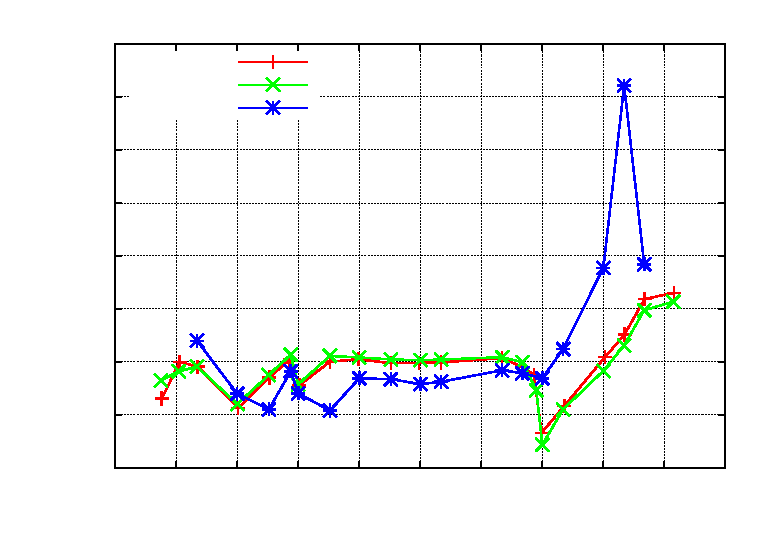
\includegraphics{../GNU/Mega8cap}}%
    \gplfronttext
  \end{picture}%
\endgroup

\caption{Prozentualer Fehler der Kondensator-Messungen mit drei ATmega8}
\label{fig:mega8cap}
\end{figure}

\begin{figure}[H]
  \begin{subfigure}[b]{9cm}
    \centering
    \resizebox{9cm}{!}{% GNUPLOT: LaTeX picture with Postscript
\begingroup
  \makeatletter
  \providecommand\color[2][]{%
    \GenericError{(gnuplot) \space\space\space\@spaces}{%
      Package color not loaded in conjunction with
      terminal option `colourtext'%
    }{See the gnuplot documentation for explanation.%
    }{Either use 'blacktext' in gnuplot or load the package
      color.sty in LaTeX.}%
    \renewcommand\color[2][]{}%
  }%
  \providecommand\includegraphics[2][]{%
    \GenericError{(gnuplot) \space\space\space\@spaces}{%
      Package graphicx or graphics not loaded%
    }{See the gnuplot documentation for explanation.%
    }{The gnuplot epslatex terminal needs graphicx.sty or graphics.sty.}%
    \renewcommand\includegraphics[2][]{}%
  }%
  \providecommand\rotatebox[2]{#2}%
  \@ifundefined{ifGPcolor}{%
    \newif\ifGPcolor
    \GPcolortrue
  }{}%
  \@ifundefined{ifGPblacktext}{%
    \newif\ifGPblacktext
    \GPblacktexttrue
  }{}%
  % define a \g@addto@macro without @ in the name:
  \let\gplgaddtomacro\g@addto@macro
  % define empty templates for all commands taking text:
  \gdef\gplbacktext{}%
  \gdef\gplfronttext{}%
  \makeatother
  \ifGPblacktext
    % no textcolor at all
    \def\colorrgb#1{}%
    \def\colorgray#1{}%
  \else
    % gray or color?
    \ifGPcolor
      \def\colorrgb#1{\color[rgb]{#1}}%
      \def\colorgray#1{\color[gray]{#1}}%
      \expandafter\def\csname LTw\endcsname{\color{white}}%
      \expandafter\def\csname LTb\endcsname{\color{black}}%
      \expandafter\def\csname LTa\endcsname{\color{black}}%
      \expandafter\def\csname LT0\endcsname{\color[rgb]{1,0,0}}%
      \expandafter\def\csname LT1\endcsname{\color[rgb]{0,1,0}}%
      \expandafter\def\csname LT2\endcsname{\color[rgb]{0,0,1}}%
      \expandafter\def\csname LT3\endcsname{\color[rgb]{1,0,1}}%
      \expandafter\def\csname LT4\endcsname{\color[rgb]{0,1,1}}%
      \expandafter\def\csname LT5\endcsname{\color[rgb]{1,1,0}}%
      \expandafter\def\csname LT6\endcsname{\color[rgb]{0,0,0}}%
      \expandafter\def\csname LT7\endcsname{\color[rgb]{1,0.3,0}}%
      \expandafter\def\csname LT8\endcsname{\color[rgb]{0.5,0.5,0.5}}%
    \else
      % gray
      \def\colorrgb#1{\color{black}}%
      \def\colorgray#1{\color[gray]{#1}}%
      \expandafter\def\csname LTw\endcsname{\color{white}}%
      \expandafter\def\csname LTb\endcsname{\color{black}}%
      \expandafter\def\csname LTa\endcsname{\color{black}}%
      \expandafter\def\csname LT0\endcsname{\color{black}}%
      \expandafter\def\csname LT1\endcsname{\color{black}}%
      \expandafter\def\csname LT2\endcsname{\color{black}}%
      \expandafter\def\csname LT3\endcsname{\color{black}}%
      \expandafter\def\csname LT4\endcsname{\color{black}}%
      \expandafter\def\csname LT5\endcsname{\color{black}}%
      \expandafter\def\csname LT6\endcsname{\color{black}}%
      \expandafter\def\csname LT7\endcsname{\color{black}}%
      \expandafter\def\csname LT8\endcsname{\color{black}}%
    \fi
  \fi
  \setlength{\unitlength}{0.0500bp}%
  \begin{picture}(7200.00,5040.00)%
    \gplgaddtomacro\gplbacktext{%
      \csname LTb\endcsname%
      \put(814,704){\makebox(0,0)[r]{\strut{}-2}}%
      \csname LTb\endcsname%
      \put(814,1383){\makebox(0,0)[r]{\strut{} 0}}%
      \csname LTb\endcsname%
      \put(814,2061){\makebox(0,0)[r]{\strut{} 2}}%
      \csname LTb\endcsname%
      \put(814,2740){\makebox(0,0)[r]{\strut{} 4}}%
      \csname LTb\endcsname%
      \put(814,3418){\makebox(0,0)[r]{\strut{} 6}}%
      \csname LTb\endcsname%
      \put(814,4097){\makebox(0,0)[r]{\strut{} 8}}%
      \csname LTb\endcsname%
      \put(814,4775){\makebox(0,0)[r]{\strut{} 10}}%
      \csname LTb\endcsname%
      \put(946,484){\makebox(0,0){\strut{}10p}}%
      \csname LTb\endcsname%
      \put(1532,484){\makebox(0,0){\strut{}100p}}%
      \csname LTb\endcsname%
      \put(2117,484){\makebox(0,0){\strut{}1n}}%
      \csname LTb\endcsname%
      \put(2703,484){\makebox(0,0){\strut{}10n}}%
      \csname LTb\endcsname%
      \put(3289,484){\makebox(0,0){\strut{}100n}}%
      \csname LTb\endcsname%
      \put(3875,484){\makebox(0,0){\strut{}1u}}%
      \csname LTb\endcsname%
      \put(4460,484){\makebox(0,0){\strut{}10u}}%
      \csname LTb\endcsname%
      \put(5046,484){\makebox(0,0){\strut{}100u}}%
      \csname LTb\endcsname%
      \put(5632,484){\makebox(0,0){\strut{}1m}}%
      \csname LTb\endcsname%
      \put(6217,484){\makebox(0,0){\strut{}10m}}%
      \csname LTb\endcsname%
      \put(6803,484){\makebox(0,0){\strut{}100m}}%
      \put(176,2739){\rotatebox{-270}{\makebox(0,0){\strut{}Error / Percent}}}%
      \put(3874,154){\makebox(0,0){\strut{}Capacity value / F}}%
      \put(3874,4665){\makebox(0,0){\strut{}}}%
    }%
    \gplgaddtomacro\gplfronttext{%
      \csname LTb\endcsname%
      \put(2134,4602){\makebox(0,0)[r]{\strut{}Mega8A-4}}%
      \csname LTb\endcsname%
      \put(2134,4382){\makebox(0,0)[r]{\strut{}Mega8A-5}}%
      \csname LTb\endcsname%
      \put(2134,4162){\makebox(0,0)[r]{\strut{}Mega8A-6}}%
    }%
    \gplbacktext
    \put(0,0){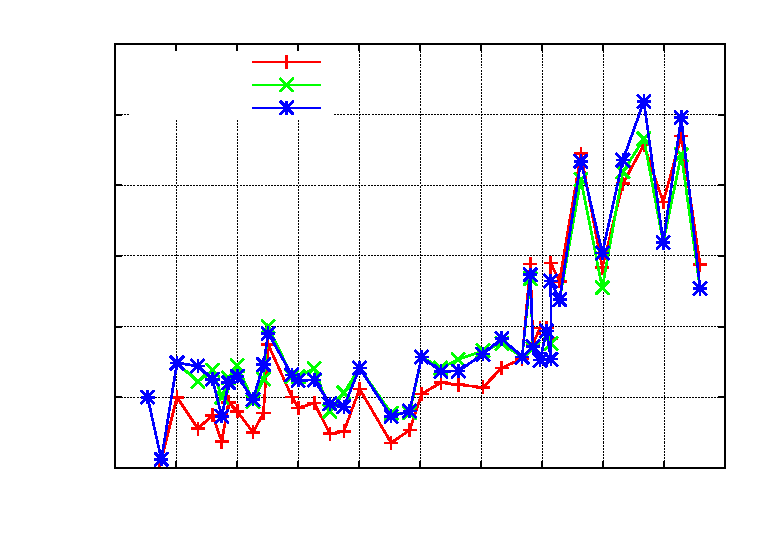
\includegraphics{../GNU/Mega8Acap}}%
    \gplfronttext
  \end{picture}%
\endgroup
}
    \caption{mit drei ATmega8A}
    \label{fig:mega8Acap}
  \end{subfigure}
  ~
  \begin{subfigure}[b]{9cm}
    \centering
    \resizebox{9cm}{!}{% GNUPLOT: LaTeX picture with Postscript
\begingroup
  \makeatletter
  \providecommand\color[2][]{%
    \GenericError{(gnuplot) \space\space\space\@spaces}{%
      Package color not loaded in conjunction with
      terminal option `colourtext'%
    }{See the gnuplot documentation for explanation.%
    }{Either use 'blacktext' in gnuplot or load the package
      color.sty in LaTeX.}%
    \renewcommand\color[2][]{}%
  }%
  \providecommand\includegraphics[2][]{%
    \GenericError{(gnuplot) \space\space\space\@spaces}{%
      Package graphicx or graphics not loaded%
    }{See the gnuplot documentation for explanation.%
    }{The gnuplot epslatex terminal needs graphicx.sty or graphics.sty.}%
    \renewcommand\includegraphics[2][]{}%
  }%
  \providecommand\rotatebox[2]{#2}%
  \@ifundefined{ifGPcolor}{%
    \newif\ifGPcolor
    \GPcolortrue
  }{}%
  \@ifundefined{ifGPblacktext}{%
    \newif\ifGPblacktext
    \GPblacktexttrue
  }{}%
  % define a \g@addto@macro without @ in the name:
  \let\gplgaddtomacro\g@addto@macro
  % define empty templates for all commands taking text:
  \gdef\gplbacktext{}%
  \gdef\gplfronttext{}%
  \makeatother
  \ifGPblacktext
    % no textcolor at all
    \def\colorrgb#1{}%
    \def\colorgray#1{}%
  \else
    % gray or color?
    \ifGPcolor
      \def\colorrgb#1{\color[rgb]{#1}}%
      \def\colorgray#1{\color[gray]{#1}}%
      \expandafter\def\csname LTw\endcsname{\color{white}}%
      \expandafter\def\csname LTb\endcsname{\color{black}}%
      \expandafter\def\csname LTa\endcsname{\color{black}}%
      \expandafter\def\csname LT0\endcsname{\color[rgb]{1,0,0}}%
      \expandafter\def\csname LT1\endcsname{\color[rgb]{0,1,0}}%
      \expandafter\def\csname LT2\endcsname{\color[rgb]{0,0,1}}%
      \expandafter\def\csname LT3\endcsname{\color[rgb]{1,0,1}}%
      \expandafter\def\csname LT4\endcsname{\color[rgb]{0,1,1}}%
      \expandafter\def\csname LT5\endcsname{\color[rgb]{1,1,0}}%
      \expandafter\def\csname LT6\endcsname{\color[rgb]{0,0,0}}%
      \expandafter\def\csname LT7\endcsname{\color[rgb]{1,0.3,0}}%
      \expandafter\def\csname LT8\endcsname{\color[rgb]{0.5,0.5,0.5}}%
    \else
      % gray
      \def\colorrgb#1{\color{black}}%
      \def\colorgray#1{\color[gray]{#1}}%
      \expandafter\def\csname LTw\endcsname{\color{white}}%
      \expandafter\def\csname LTb\endcsname{\color{black}}%
      \expandafter\def\csname LTa\endcsname{\color{black}}%
      \expandafter\def\csname LT0\endcsname{\color{black}}%
      \expandafter\def\csname LT1\endcsname{\color{black}}%
      \expandafter\def\csname LT2\endcsname{\color{black}}%
      \expandafter\def\csname LT3\endcsname{\color{black}}%
      \expandafter\def\csname LT4\endcsname{\color{black}}%
      \expandafter\def\csname LT5\endcsname{\color{black}}%
      \expandafter\def\csname LT6\endcsname{\color{black}}%
      \expandafter\def\csname LT7\endcsname{\color{black}}%
      \expandafter\def\csname LT8\endcsname{\color{black}}%
    \fi
  \fi
  \setlength{\unitlength}{0.0500bp}%
  \begin{picture}(7200.00,5040.00)%
    \gplgaddtomacro\gplbacktext{%
      \csname LTb\endcsname%
      \put(814,704){\makebox(0,0)[r]{\strut{}-2}}%
      \csname LTb\endcsname%
      \put(814,1383){\makebox(0,0)[r]{\strut{} 0}}%
      \csname LTb\endcsname%
      \put(814,2061){\makebox(0,0)[r]{\strut{} 2}}%
      \csname LTb\endcsname%
      \put(814,2740){\makebox(0,0)[r]{\strut{} 4}}%
      \csname LTb\endcsname%
      \put(814,3418){\makebox(0,0)[r]{\strut{} 6}}%
      \csname LTb\endcsname%
      \put(814,4097){\makebox(0,0)[r]{\strut{} 8}}%
      \csname LTb\endcsname%
      \put(814,4775){\makebox(0,0)[r]{\strut{} 10}}%
      \csname LTb\endcsname%
      \put(946,484){\makebox(0,0){\strut{}10p}}%
      \csname LTb\endcsname%
      \put(1532,484){\makebox(0,0){\strut{}100p}}%
      \csname LTb\endcsname%
      \put(2117,484){\makebox(0,0){\strut{}1n}}%
      \csname LTb\endcsname%
      \put(2703,484){\makebox(0,0){\strut{}10n}}%
      \csname LTb\endcsname%
      \put(3289,484){\makebox(0,0){\strut{}100n}}%
      \csname LTb\endcsname%
      \put(3875,484){\makebox(0,0){\strut{}1u}}%
      \csname LTb\endcsname%
      \put(4460,484){\makebox(0,0){\strut{}10u}}%
      \csname LTb\endcsname%
      \put(5046,484){\makebox(0,0){\strut{}100u}}%
      \csname LTb\endcsname%
      \put(5632,484){\makebox(0,0){\strut{}1m}}%
      \csname LTb\endcsname%
      \put(6217,484){\makebox(0,0){\strut{}10m}}%
      \csname LTb\endcsname%
      \put(6803,484){\makebox(0,0){\strut{}100m}}%
      \put(176,2739){\rotatebox{-270}{\makebox(0,0){\strut{}Error / Percent}}}%
      \put(3874,154){\makebox(0,0){\strut{}Capacity value / F}}%
      \put(3874,4665){\makebox(0,0){\strut{}}}%
    }%
    \gplgaddtomacro\gplfronttext{%
      \csname LTb\endcsname%
      \put(2134,4602){\makebox(0,0)[r]{\strut{}Mega8L-7}}%
      \csname LTb\endcsname%
      \put(2134,4382){\makebox(0,0)[r]{\strut{}Mega8L-8}}%
      \csname LTb\endcsname%
      \put(2134,4162){\makebox(0,0)[r]{\strut{}Mega8L-9}}%
    }%
    \gplbacktext
    \put(0,0){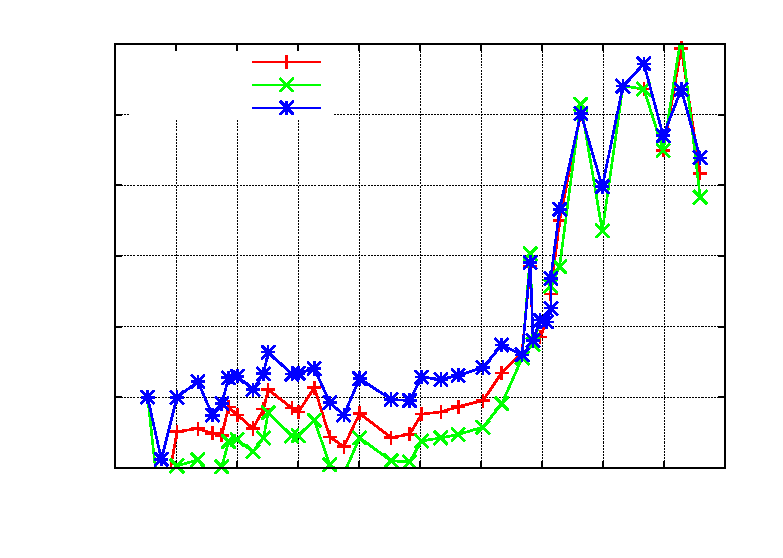
\includegraphics{../GNU/Mega8Lcap}}%
    \gplfronttext
  \end{picture}%
\endgroup
}
    \caption{mit drei ATmega8L}
    \label{fig:mega8Lcap}
  \end{subfigure}
  \caption{Prozentualer Kondensator-Messfehler}
\end{figure}

\begin{figure}[H]
\centering
% GNUPLOT: LaTeX picture with Postscript
\begingroup
  \makeatletter
  \providecommand\color[2][]{%
    \GenericError{(gnuplot) \space\space\space\@spaces}{%
      Package color not loaded in conjunction with
      terminal option `colourtext'%
    }{See the gnuplot documentation for explanation.%
    }{Either use 'blacktext' in gnuplot or load the package
      color.sty in LaTeX.}%
    \renewcommand\color[2][]{}%
  }%
  \providecommand\includegraphics[2][]{%
    \GenericError{(gnuplot) \space\space\space\@spaces}{%
      Package graphicx or graphics not loaded%
    }{See the gnuplot documentation for explanation.%
    }{The gnuplot epslatex terminal needs graphicx.sty or graphics.sty.}%
    \renewcommand\includegraphics[2][]{}%
  }%
  \providecommand\rotatebox[2]{#2}%
  \@ifundefined{ifGPcolor}{%
    \newif\ifGPcolor
    \GPcolortrue
  }{}%
  \@ifundefined{ifGPblacktext}{%
    \newif\ifGPblacktext
    \GPblacktexttrue
  }{}%
  % define a \g@addto@macro without @ in the name:
  \let\gplgaddtomacro\g@addto@macro
  % define empty templates for all commands taking text:
  \gdef\gplbacktext{}%
  \gdef\gplfronttext{}%
  \makeatother
  \ifGPblacktext
    % no textcolor at all
    \def\colorrgb#1{}%
    \def\colorgray#1{}%
  \else
    % gray or color?
    \ifGPcolor
      \def\colorrgb#1{\color[rgb]{#1}}%
      \def\colorgray#1{\color[gray]{#1}}%
      \expandafter\def\csname LTw\endcsname{\color{white}}%
      \expandafter\def\csname LTb\endcsname{\color{black}}%
      \expandafter\def\csname LTa\endcsname{\color{black}}%
      \expandafter\def\csname LT0\endcsname{\color[rgb]{1,0,0}}%
      \expandafter\def\csname LT1\endcsname{\color[rgb]{0,1,0}}%
      \expandafter\def\csname LT2\endcsname{\color[rgb]{0,0,1}}%
      \expandafter\def\csname LT3\endcsname{\color[rgb]{1,0,1}}%
      \expandafter\def\csname LT4\endcsname{\color[rgb]{0,1,1}}%
      \expandafter\def\csname LT5\endcsname{\color[rgb]{1,1,0}}%
      \expandafter\def\csname LT6\endcsname{\color[rgb]{0,0,0}}%
      \expandafter\def\csname LT7\endcsname{\color[rgb]{1,0.3,0}}%
      \expandafter\def\csname LT8\endcsname{\color[rgb]{0.5,0.5,0.5}}%
    \else
      % gray
      \def\colorrgb#1{\color{black}}%
      \def\colorgray#1{\color[gray]{#1}}%
      \expandafter\def\csname LTw\endcsname{\color{white}}%
      \expandafter\def\csname LTb\endcsname{\color{black}}%
      \expandafter\def\csname LTa\endcsname{\color{black}}%
      \expandafter\def\csname LT0\endcsname{\color{black}}%
      \expandafter\def\csname LT1\endcsname{\color{black}}%
      \expandafter\def\csname LT2\endcsname{\color{black}}%
      \expandafter\def\csname LT3\endcsname{\color{black}}%
      \expandafter\def\csname LT4\endcsname{\color{black}}%
      \expandafter\def\csname LT5\endcsname{\color{black}}%
      \expandafter\def\csname LT6\endcsname{\color{black}}%
      \expandafter\def\csname LT7\endcsname{\color{black}}%
      \expandafter\def\csname LT8\endcsname{\color{black}}%
    \fi
  \fi
  \setlength{\unitlength}{0.0500bp}%
  \begin{picture}(7200.00,5040.00)%
    \gplgaddtomacro\gplbacktext{%
      \csname LTb\endcsname%
      \put(814,704){\makebox(0,0)[r]{\strut{}-2}}%
      \csname LTb\endcsname%
      \put(814,1383){\makebox(0,0)[r]{\strut{} 0}}%
      \csname LTb\endcsname%
      \put(814,2061){\makebox(0,0)[r]{\strut{} 2}}%
      \csname LTb\endcsname%
      \put(814,2740){\makebox(0,0)[r]{\strut{} 4}}%
      \csname LTb\endcsname%
      \put(814,3418){\makebox(0,0)[r]{\strut{} 6}}%
      \csname LTb\endcsname%
      \put(814,4097){\makebox(0,0)[r]{\strut{} 8}}%
      \csname LTb\endcsname%
      \put(814,4775){\makebox(0,0)[r]{\strut{} 10}}%
      \csname LTb\endcsname%
      \put(946,484){\makebox(0,0){\strut{}10p}}%
      \csname LTb\endcsname%
      \put(1532,484){\makebox(0,0){\strut{}100p}}%
      \csname LTb\endcsname%
      \put(2117,484){\makebox(0,0){\strut{}1n}}%
      \csname LTb\endcsname%
      \put(2703,484){\makebox(0,0){\strut{}10n}}%
      \csname LTb\endcsname%
      \put(3289,484){\makebox(0,0){\strut{}100n}}%
      \csname LTb\endcsname%
      \put(3875,484){\makebox(0,0){\strut{}1u}}%
      \csname LTb\endcsname%
      \put(4460,484){\makebox(0,0){\strut{}10u}}%
      \csname LTb\endcsname%
      \put(5046,484){\makebox(0,0){\strut{}100u}}%
      \csname LTb\endcsname%
      \put(5632,484){\makebox(0,0){\strut{}1m}}%
      \csname LTb\endcsname%
      \put(6217,484){\makebox(0,0){\strut{}10m}}%
      \csname LTb\endcsname%
      \put(6803,484){\makebox(0,0){\strut{}100m}}%
      \put(176,2739){\rotatebox{-270}{\makebox(0,0){\strut{}Error / Percent}}}%
      \put(3874,154){\makebox(0,0){\strut{}Capacity value / F}}%
      \put(3874,4665){\makebox(0,0){\strut{}}}%
    }%
    \gplgaddtomacro\gplfronttext{%
      \csname LTb\endcsname%
      \put(2398,4602){\makebox(0,0)[r]{\strut{}Mega168}}%
      \csname LTb\endcsname%
      \put(2398,4382){\makebox(0,0)[r]{\strut{}Mega168as8}}%
    }%
    \gplbacktext
    \put(0,0){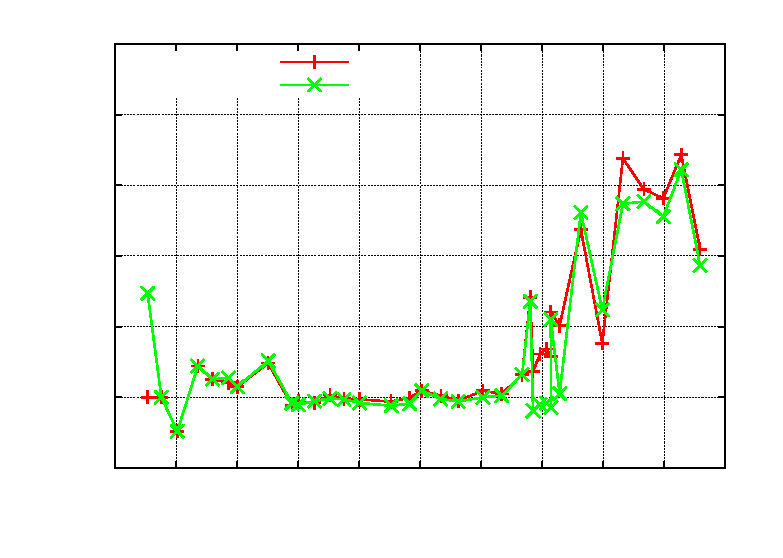
\includegraphics{../GNU/Mega168cap}}%
    \gplfronttext
  \end{picture}%
\endgroup

\caption{Prozentualer Fehler der Kondensator-Messungen mit dem ATmega168}
\label{fig:mega168cap}
\end{figure}

Wie schwierig es ist, für Kondensatormessungen den richtigen Bezugswert zu finden, soll die Abbildung~\ref{fig:capcompare} zeigen.
Als Bezugswert wurde hier eine beste Schätzung genommen. Die Kurve ,,Multimeter'' zeigt die Abweichungen, die mit einem
Peaktech~3315 Multimeter gemessen wurden.
Die nächste Kurve ,,LCR'' zeigt die Abweichungen, die mit einem Peaktech~2170 LCR-Meter in dem jeweils günstigsten Frequenzbereich gemessen wurden.
Zum Vergleich werden mit der Kurve ,,ATmega168as'' auch noch die Messabweichungen eines ATmega168 bestücktem Transistor-Testers gezeigt.
Ob die gezeigten Fehler aber tatsächliche Messfehler des jeweiligen Gerätes sind, muss bezweifelt werden, da auch die
Schätzung des Kapazitätswert nicht der wirklichen Kapazität entspricht.

\begin{figure}[H]
\centering
% GNUPLOT: LaTeX picture with Postscript
\begingroup
  \makeatletter
  \providecommand\color[2][]{%
    \GenericError{(gnuplot) \space\space\space\@spaces}{%
      Package color not loaded in conjunction with
      terminal option `colourtext'%
    }{See the gnuplot documentation for explanation.%
    }{Either use 'blacktext' in gnuplot or load the package
      color.sty in LaTeX.}%
    \renewcommand\color[2][]{}%
  }%
  \providecommand\includegraphics[2][]{%
    \GenericError{(gnuplot) \space\space\space\@spaces}{%
      Package graphicx or graphics not loaded%
    }{See the gnuplot documentation for explanation.%
    }{The gnuplot epslatex terminal needs graphicx.sty or graphics.sty.}%
    \renewcommand\includegraphics[2][]{}%
  }%
  \providecommand\rotatebox[2]{#2}%
  \@ifundefined{ifGPcolor}{%
    \newif\ifGPcolor
    \GPcolortrue
  }{}%
  \@ifundefined{ifGPblacktext}{%
    \newif\ifGPblacktext
    \GPblacktexttrue
  }{}%
  % define a \g@addto@macro without @ in the name:
  \let\gplgaddtomacro\g@addto@macro
  % define empty templates for all commands taking text:
  \gdef\gplbacktext{}%
  \gdef\gplfronttext{}%
  \makeatother
  \ifGPblacktext
    % no textcolor at all
    \def\colorrgb#1{}%
    \def\colorgray#1{}%
  \else
    % gray or color?
    \ifGPcolor
      \def\colorrgb#1{\color[rgb]{#1}}%
      \def\colorgray#1{\color[gray]{#1}}%
      \expandafter\def\csname LTw\endcsname{\color{white}}%
      \expandafter\def\csname LTb\endcsname{\color{black}}%
      \expandafter\def\csname LTa\endcsname{\color{black}}%
      \expandafter\def\csname LT0\endcsname{\color[rgb]{1,0,0}}%
      \expandafter\def\csname LT1\endcsname{\color[rgb]{0,1,0}}%
      \expandafter\def\csname LT2\endcsname{\color[rgb]{0,0,1}}%
      \expandafter\def\csname LT3\endcsname{\color[rgb]{1,0,1}}%
      \expandafter\def\csname LT4\endcsname{\color[rgb]{0,1,1}}%
      \expandafter\def\csname LT5\endcsname{\color[rgb]{1,1,0}}%
      \expandafter\def\csname LT6\endcsname{\color[rgb]{0,0,0}}%
      \expandafter\def\csname LT7\endcsname{\color[rgb]{1,0.3,0}}%
      \expandafter\def\csname LT8\endcsname{\color[rgb]{0.5,0.5,0.5}}%
    \else
      % gray
      \def\colorrgb#1{\color{black}}%
      \def\colorgray#1{\color[gray]{#1}}%
      \expandafter\def\csname LTw\endcsname{\color{white}}%
      \expandafter\def\csname LTb\endcsname{\color{black}}%
      \expandafter\def\csname LTa\endcsname{\color{black}}%
      \expandafter\def\csname LT0\endcsname{\color{black}}%
      \expandafter\def\csname LT1\endcsname{\color{black}}%
      \expandafter\def\csname LT2\endcsname{\color{black}}%
      \expandafter\def\csname LT3\endcsname{\color{black}}%
      \expandafter\def\csname LT4\endcsname{\color{black}}%
      \expandafter\def\csname LT5\endcsname{\color{black}}%
      \expandafter\def\csname LT6\endcsname{\color{black}}%
      \expandafter\def\csname LT7\endcsname{\color{black}}%
      \expandafter\def\csname LT8\endcsname{\color{black}}%
    \fi
  \fi
  \setlength{\unitlength}{0.0500bp}%
  \begin{picture}(7200.00,5040.00)%
    \gplgaddtomacro\gplbacktext{%
      \csname LTb\endcsname%
      \put(814,704){\makebox(0,0)[r]{\strut{}-10}}%
      \csname LTb\endcsname%
      \put(814,1111){\makebox(0,0)[r]{\strut{}-8}}%
      \csname LTb\endcsname%
      \put(814,1518){\makebox(0,0)[r]{\strut{}-6}}%
      \csname LTb\endcsname%
      \put(814,1925){\makebox(0,0)[r]{\strut{}-4}}%
      \csname LTb\endcsname%
      \put(814,2332){\makebox(0,0)[r]{\strut{}-2}}%
      \csname LTb\endcsname%
      \put(814,2740){\makebox(0,0)[r]{\strut{} 0}}%
      \csname LTb\endcsname%
      \put(814,3147){\makebox(0,0)[r]{\strut{} 2}}%
      \csname LTb\endcsname%
      \put(814,3554){\makebox(0,0)[r]{\strut{} 4}}%
      \csname LTb\endcsname%
      \put(814,3961){\makebox(0,0)[r]{\strut{} 6}}%
      \csname LTb\endcsname%
      \put(814,4368){\makebox(0,0)[r]{\strut{} 8}}%
      \csname LTb\endcsname%
      \put(814,4775){\makebox(0,0)[r]{\strut{} 10}}%
      \csname LTb\endcsname%
      \put(946,484){\makebox(0,0){\strut{}10p}}%
      \csname LTb\endcsname%
      \put(1532,484){\makebox(0,0){\strut{}100p}}%
      \csname LTb\endcsname%
      \put(2117,484){\makebox(0,0){\strut{}1n}}%
      \csname LTb\endcsname%
      \put(2703,484){\makebox(0,0){\strut{}10n}}%
      \csname LTb\endcsname%
      \put(3289,484){\makebox(0,0){\strut{}100n}}%
      \csname LTb\endcsname%
      \put(3875,484){\makebox(0,0){\strut{}1u}}%
      \csname LTb\endcsname%
      \put(4460,484){\makebox(0,0){\strut{}10u}}%
      \csname LTb\endcsname%
      \put(5046,484){\makebox(0,0){\strut{}100u}}%
      \csname LTb\endcsname%
      \put(5632,484){\makebox(0,0){\strut{}1m}}%
      \csname LTb\endcsname%
      \put(6217,484){\makebox(0,0){\strut{}10m}}%
      \csname LTb\endcsname%
      \put(6803,484){\makebox(0,0){\strut{}100m}}%
      \put(176,2739){\rotatebox{-270}{\makebox(0,0){\strut{}Error / Percent}}}%
      \put(3874,154){\makebox(0,0){\strut{}Capacity value / F}}%
      \put(3874,4665){\makebox(0,0){\strut{}}}%
    }%
    \gplgaddtomacro\gplfronttext{%
      \csname LTb\endcsname%
      \put(2398,4602){\makebox(0,0)[r]{\strut{}Multimeter}}%
      \csname LTb\endcsname%
      \put(2398,4382){\makebox(0,0)[r]{\strut{}LCR}}%
      \csname LTb\endcsname%
      \put(2398,4162){\makebox(0,0)[r]{\strut{}Mega168as}}%
    }%
    \gplbacktext
    \put(0,0){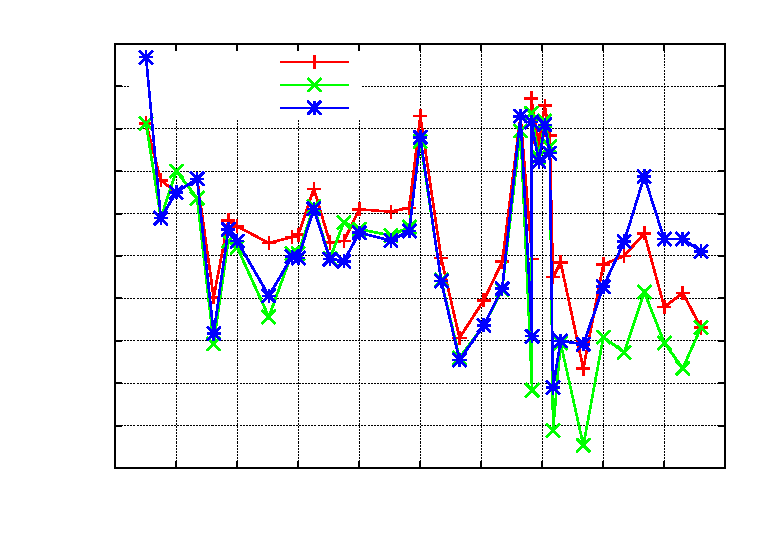
\includegraphics{../GNU/capcompare}}%
    \gplfronttext
  \end{picture}%
\endgroup

\caption{Vergleich der Kondensator-Messungen mit Multimeter, LCR-Meter und ATmega168}
\label{fig:capcompare}
\end{figure}

Die Abweichungen der Messergebnisse von drei verschiedenen ATmega168 werden in Abbildung~\ref{fig:mega168all} dargestellt.
Hier wurde die Messung des LCR-Meters als Vergleichsbasis genommen.
Entsprechend werden die Messergebnisse von drei verschiedenen ATmega168A in Abbildung~\ref{fig:mega168Aall}, 
von drei verschiedenen ATmega168PA in Abbildung~\ref{fig:mega168PAall} und von drei verschiedenen
ATmega328 in Abbildung~\ref{fig:mega328all} sowie von drei ATmega328P in Abbildung~\ref{fig:mega328Pall} gezeigt.
Hierbei wurde nur der Nullwert der Kapazitätsmessung von 39pF berücksichtigt, alle anderen Korrekturmöglichkeiten wurden
nicht benutzt. Dieser Nullwert beinhaltet schon die 2-3pF, die durch die etwa 12~cm langen Anschlussleitungen mit den
Klemmen verursacht werden.
Auch das Board-Layout hat Einfluss auf diesen Nullwert. Diesen Nullwert habe ich mit der Boardversion ,,DG2BRS V 5.2.1'' ermittelt.

\begin{figure}[H]
  \begin{subfigure}[b]{9cm}
    \centering
    \resizebox{9cm}{!}{% GNUPLOT: LaTeX picture with Postscript
\begingroup
  \makeatletter
  \providecommand\color[2][]{%
    \GenericError{(gnuplot) \space\space\space\@spaces}{%
      Package color not loaded in conjunction with
      terminal option `colourtext'%
    }{See the gnuplot documentation for explanation.%
    }{Either use 'blacktext' in gnuplot or load the package
      color.sty in LaTeX.}%
    \renewcommand\color[2][]{}%
  }%
  \providecommand\includegraphics[2][]{%
    \GenericError{(gnuplot) \space\space\space\@spaces}{%
      Package graphicx or graphics not loaded%
    }{See the gnuplot documentation for explanation.%
    }{The gnuplot epslatex terminal needs graphicx.sty or graphics.sty.}%
    \renewcommand\includegraphics[2][]{}%
  }%
  \providecommand\rotatebox[2]{#2}%
  \@ifundefined{ifGPcolor}{%
    \newif\ifGPcolor
    \GPcolortrue
  }{}%
  \@ifundefined{ifGPblacktext}{%
    \newif\ifGPblacktext
    \GPblacktexttrue
  }{}%
  % define a \g@addto@macro without @ in the name:
  \let\gplgaddtomacro\g@addto@macro
  % define empty templates for all commands taking text:
  \gdef\gplbacktext{}%
  \gdef\gplfronttext{}%
  \makeatother
  \ifGPblacktext
    % no textcolor at all
    \def\colorrgb#1{}%
    \def\colorgray#1{}%
  \else
    % gray or color?
    \ifGPcolor
      \def\colorrgb#1{\color[rgb]{#1}}%
      \def\colorgray#1{\color[gray]{#1}}%
      \expandafter\def\csname LTw\endcsname{\color{white}}%
      \expandafter\def\csname LTb\endcsname{\color{black}}%
      \expandafter\def\csname LTa\endcsname{\color{black}}%
      \expandafter\def\csname LT0\endcsname{\color[rgb]{1,0,0}}%
      \expandafter\def\csname LT1\endcsname{\color[rgb]{0,1,0}}%
      \expandafter\def\csname LT2\endcsname{\color[rgb]{0,0,1}}%
      \expandafter\def\csname LT3\endcsname{\color[rgb]{1,0,1}}%
      \expandafter\def\csname LT4\endcsname{\color[rgb]{0,1,1}}%
      \expandafter\def\csname LT5\endcsname{\color[rgb]{1,1,0}}%
      \expandafter\def\csname LT6\endcsname{\color[rgb]{0,0,0}}%
      \expandafter\def\csname LT7\endcsname{\color[rgb]{1,0.3,0}}%
      \expandafter\def\csname LT8\endcsname{\color[rgb]{0.5,0.5,0.5}}%
    \else
      % gray
      \def\colorrgb#1{\color{black}}%
      \def\colorgray#1{\color[gray]{#1}}%
      \expandafter\def\csname LTw\endcsname{\color{white}}%
      \expandafter\def\csname LTb\endcsname{\color{black}}%
      \expandafter\def\csname LTa\endcsname{\color{black}}%
      \expandafter\def\csname LT0\endcsname{\color{black}}%
      \expandafter\def\csname LT1\endcsname{\color{black}}%
      \expandafter\def\csname LT2\endcsname{\color{black}}%
      \expandafter\def\csname LT3\endcsname{\color{black}}%
      \expandafter\def\csname LT4\endcsname{\color{black}}%
      \expandafter\def\csname LT5\endcsname{\color{black}}%
      \expandafter\def\csname LT6\endcsname{\color{black}}%
      \expandafter\def\csname LT7\endcsname{\color{black}}%
      \expandafter\def\csname LT8\endcsname{\color{black}}%
    \fi
  \fi
  \setlength{\unitlength}{0.0500bp}%
  \begin{picture}(7200.00,5040.00)%
    \gplgaddtomacro\gplbacktext{%
      \csname LTb\endcsname%
      \put(814,704){\makebox(0,0)[r]{\strut{}-4}}%
      \csname LTb\endcsname%
      \put(814,1111){\makebox(0,0)[r]{\strut{}-2}}%
      \csname LTb\endcsname%
      \put(814,1518){\makebox(0,0)[r]{\strut{} 0}}%
      \csname LTb\endcsname%
      \put(814,1925){\makebox(0,0)[r]{\strut{} 2}}%
      \csname LTb\endcsname%
      \put(814,2332){\makebox(0,0)[r]{\strut{} 4}}%
      \csname LTb\endcsname%
      \put(814,2740){\makebox(0,0)[r]{\strut{} 6}}%
      \csname LTb\endcsname%
      \put(814,3147){\makebox(0,0)[r]{\strut{} 8}}%
      \csname LTb\endcsname%
      \put(814,3554){\makebox(0,0)[r]{\strut{} 10}}%
      \csname LTb\endcsname%
      \put(814,3961){\makebox(0,0)[r]{\strut{} 12}}%
      \csname LTb\endcsname%
      \put(814,4368){\makebox(0,0)[r]{\strut{} 14}}%
      \csname LTb\endcsname%
      \put(814,4775){\makebox(0,0)[r]{\strut{} 16}}%
      \csname LTb\endcsname%
      \put(946,484){\makebox(0,0){\strut{}10p}}%
      \csname LTb\endcsname%
      \put(1597,484){\makebox(0,0){\strut{}100p}}%
      \csname LTb\endcsname%
      \put(2248,484){\makebox(0,0){\strut{}1n}}%
      \csname LTb\endcsname%
      \put(2898,484){\makebox(0,0){\strut{}10n}}%
      \csname LTb\endcsname%
      \put(3549,484){\makebox(0,0){\strut{}100n}}%
      \csname LTb\endcsname%
      \put(4200,484){\makebox(0,0){\strut{}1u}}%
      \csname LTb\endcsname%
      \put(4851,484){\makebox(0,0){\strut{}10u}}%
      \csname LTb\endcsname%
      \put(5501,484){\makebox(0,0){\strut{}100u}}%
      \csname LTb\endcsname%
      \put(6152,484){\makebox(0,0){\strut{}1m}}%
      \csname LTb\endcsname%
      \put(6803,484){\makebox(0,0){\strut{}10m}}%
      \put(176,2739){\rotatebox{-270}{\makebox(0,0){\strut{}Error / Percent}}}%
      \put(3874,154){\makebox(0,0){\strut{}Capacity value / F}}%
      \put(3874,4665){\makebox(0,0){\strut{}}}%
    }%
    \gplgaddtomacro\gplfronttext{%
      \csname LTb\endcsname%
      \put(5753,4602){\makebox(0,0)[r]{\strut{}168-1}}%
      \csname LTb\endcsname%
      \put(5753,4382){\makebox(0,0)[r]{\strut{}168-2}}%
      \csname LTb\endcsname%
      \put(5753,4162){\makebox(0,0)[r]{\strut{}168-3}}%
    }%
    \gplbacktext
    \put(0,0){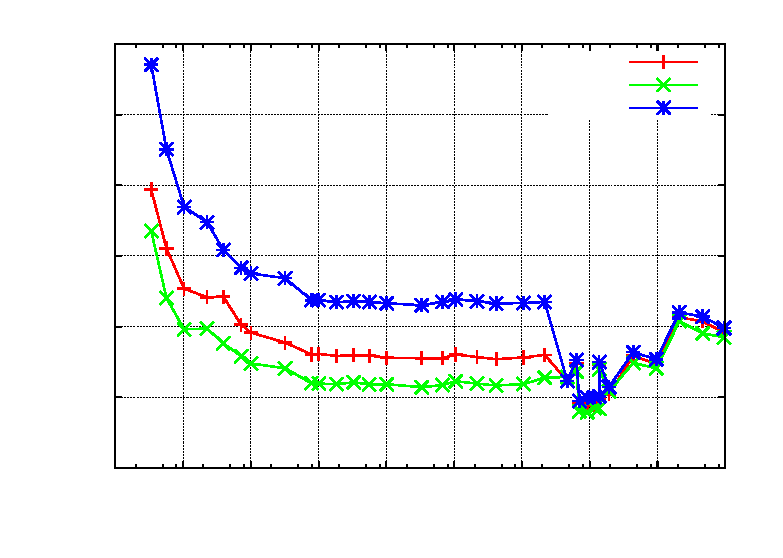
\includegraphics{../GNU/Mega168all}}%
    \gplfronttext
  \end{picture}%
\endgroup
}
    \caption{drei ATmega168}
    \label{fig:mega168all}
  \end{subfigure}
  ~
  \begin{subfigure}[b]{9cm}
    \centering
    \resizebox{9cm}{!}{% GNUPLOT: LaTeX picture with Postscript
\begingroup
  \makeatletter
  \providecommand\color[2][]{%
    \GenericError{(gnuplot) \space\space\space\@spaces}{%
      Package color not loaded in conjunction with
      terminal option `colourtext'%
    }{See the gnuplot documentation for explanation.%
    }{Either use 'blacktext' in gnuplot or load the package
      color.sty in LaTeX.}%
    \renewcommand\color[2][]{}%
  }%
  \providecommand\includegraphics[2][]{%
    \GenericError{(gnuplot) \space\space\space\@spaces}{%
      Package graphicx or graphics not loaded%
    }{See the gnuplot documentation for explanation.%
    }{The gnuplot epslatex terminal needs graphicx.sty or graphics.sty.}%
    \renewcommand\includegraphics[2][]{}%
  }%
  \providecommand\rotatebox[2]{#2}%
  \@ifundefined{ifGPcolor}{%
    \newif\ifGPcolor
    \GPcolortrue
  }{}%
  \@ifundefined{ifGPblacktext}{%
    \newif\ifGPblacktext
    \GPblacktexttrue
  }{}%
  % define a \g@addto@macro without @ in the name:
  \let\gplgaddtomacro\g@addto@macro
  % define empty templates for all commands taking text:
  \gdef\gplbacktext{}%
  \gdef\gplfronttext{}%
  \makeatother
  \ifGPblacktext
    % no textcolor at all
    \def\colorrgb#1{}%
    \def\colorgray#1{}%
  \else
    % gray or color?
    \ifGPcolor
      \def\colorrgb#1{\color[rgb]{#1}}%
      \def\colorgray#1{\color[gray]{#1}}%
      \expandafter\def\csname LTw\endcsname{\color{white}}%
      \expandafter\def\csname LTb\endcsname{\color{black}}%
      \expandafter\def\csname LTa\endcsname{\color{black}}%
      \expandafter\def\csname LT0\endcsname{\color[rgb]{1,0,0}}%
      \expandafter\def\csname LT1\endcsname{\color[rgb]{0,1,0}}%
      \expandafter\def\csname LT2\endcsname{\color[rgb]{0,0,1}}%
      \expandafter\def\csname LT3\endcsname{\color[rgb]{1,0,1}}%
      \expandafter\def\csname LT4\endcsname{\color[rgb]{0,1,1}}%
      \expandafter\def\csname LT5\endcsname{\color[rgb]{1,1,0}}%
      \expandafter\def\csname LT6\endcsname{\color[rgb]{0,0,0}}%
      \expandafter\def\csname LT7\endcsname{\color[rgb]{1,0.3,0}}%
      \expandafter\def\csname LT8\endcsname{\color[rgb]{0.5,0.5,0.5}}%
    \else
      % gray
      \def\colorrgb#1{\color{black}}%
      \def\colorgray#1{\color[gray]{#1}}%
      \expandafter\def\csname LTw\endcsname{\color{white}}%
      \expandafter\def\csname LTb\endcsname{\color{black}}%
      \expandafter\def\csname LTa\endcsname{\color{black}}%
      \expandafter\def\csname LT0\endcsname{\color{black}}%
      \expandafter\def\csname LT1\endcsname{\color{black}}%
      \expandafter\def\csname LT2\endcsname{\color{black}}%
      \expandafter\def\csname LT3\endcsname{\color{black}}%
      \expandafter\def\csname LT4\endcsname{\color{black}}%
      \expandafter\def\csname LT5\endcsname{\color{black}}%
      \expandafter\def\csname LT6\endcsname{\color{black}}%
      \expandafter\def\csname LT7\endcsname{\color{black}}%
      \expandafter\def\csname LT8\endcsname{\color{black}}%
    \fi
  \fi
  \setlength{\unitlength}{0.0500bp}%
  \begin{picture}(7200.00,5040.00)%
    \gplgaddtomacro\gplbacktext{%
      \csname LTb\endcsname%
      \put(814,704){\makebox(0,0)[r]{\strut{}-10}}%
      \csname LTb\endcsname%
      \put(814,1156){\makebox(0,0)[r]{\strut{}-8}}%
      \csname LTb\endcsname%
      \put(814,1609){\makebox(0,0)[r]{\strut{}-6}}%
      \csname LTb\endcsname%
      \put(814,2061){\makebox(0,0)[r]{\strut{}-4}}%
      \csname LTb\endcsname%
      \put(814,2513){\makebox(0,0)[r]{\strut{}-2}}%
      \csname LTb\endcsname%
      \put(814,2966){\makebox(0,0)[r]{\strut{} 0}}%
      \csname LTb\endcsname%
      \put(814,3418){\makebox(0,0)[r]{\strut{} 2}}%
      \csname LTb\endcsname%
      \put(814,3870){\makebox(0,0)[r]{\strut{} 4}}%
      \csname LTb\endcsname%
      \put(814,4323){\makebox(0,0)[r]{\strut{} 6}}%
      \csname LTb\endcsname%
      \put(814,4775){\makebox(0,0)[r]{\strut{} 8}}%
      \csname LTb\endcsname%
      \put(946,484){\makebox(0,0){\strut{}10p}}%
      \csname LTb\endcsname%
      \put(1597,484){\makebox(0,0){\strut{}100p}}%
      \csname LTb\endcsname%
      \put(2248,484){\makebox(0,0){\strut{}1n}}%
      \csname LTb\endcsname%
      \put(2898,484){\makebox(0,0){\strut{}10n}}%
      \csname LTb\endcsname%
      \put(3549,484){\makebox(0,0){\strut{}100n}}%
      \csname LTb\endcsname%
      \put(4200,484){\makebox(0,0){\strut{}1u}}%
      \csname LTb\endcsname%
      \put(4851,484){\makebox(0,0){\strut{}10u}}%
      \csname LTb\endcsname%
      \put(5501,484){\makebox(0,0){\strut{}100u}}%
      \csname LTb\endcsname%
      \put(6152,484){\makebox(0,0){\strut{}1m}}%
      \csname LTb\endcsname%
      \put(6803,484){\makebox(0,0){\strut{}10m}}%
      \put(176,2739){\rotatebox{-270}{\makebox(0,0){\strut{}Error / Percent}}}%
      \put(3874,154){\makebox(0,0){\strut{}Capacity value / F}}%
      \put(3874,4665){\makebox(0,0){\strut{}}}%
    }%
    \gplgaddtomacro\gplfronttext{%
      \csname LTb\endcsname%
      \put(3282,3987){\makebox(0,0)[r]{\strut{}168A-4}}%
      \csname LTb\endcsname%
      \put(3282,3767){\makebox(0,0)[r]{\strut{}168A-5}}%
      \csname LTb\endcsname%
      \put(3282,3547){\makebox(0,0)[r]{\strut{}168A-6}}%
    }%
    \gplbacktext
    \put(0,0){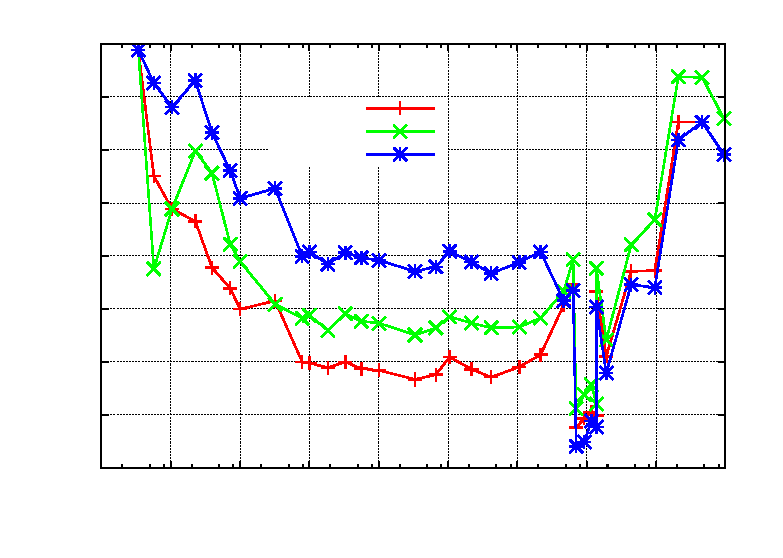
\includegraphics{../GNU/Mega168Aall}}%
    \gplfronttext
  \end{picture}%
\endgroup
}
    \caption{drei ATmega168A}
    \label{fig:mega168Aall}
  \end{subfigure}
  \caption{Kondensator-Messfehler, unkalibriert}
\end{figure}

\begin{figure}[H]
\centering
% GNUPLOT: LaTeX picture with Postscript
\begingroup
  \makeatletter
  \providecommand\color[2][]{%
    \GenericError{(gnuplot) \space\space\space\@spaces}{%
      Package color not loaded in conjunction with
      terminal option `colourtext'%
    }{See the gnuplot documentation for explanation.%
    }{Either use 'blacktext' in gnuplot or load the package
      color.sty in LaTeX.}%
    \renewcommand\color[2][]{}%
  }%
  \providecommand\includegraphics[2][]{%
    \GenericError{(gnuplot) \space\space\space\@spaces}{%
      Package graphicx or graphics not loaded%
    }{See the gnuplot documentation for explanation.%
    }{The gnuplot epslatex terminal needs graphicx.sty or graphics.sty.}%
    \renewcommand\includegraphics[2][]{}%
  }%
  \providecommand\rotatebox[2]{#2}%
  \@ifundefined{ifGPcolor}{%
    \newif\ifGPcolor
    \GPcolortrue
  }{}%
  \@ifundefined{ifGPblacktext}{%
    \newif\ifGPblacktext
    \GPblacktexttrue
  }{}%
  % define a \g@addto@macro without @ in the name:
  \let\gplgaddtomacro\g@addto@macro
  % define empty templates for all commands taking text:
  \gdef\gplbacktext{}%
  \gdef\gplfronttext{}%
  \makeatother
  \ifGPblacktext
    % no textcolor at all
    \def\colorrgb#1{}%
    \def\colorgray#1{}%
  \else
    % gray or color?
    \ifGPcolor
      \def\colorrgb#1{\color[rgb]{#1}}%
      \def\colorgray#1{\color[gray]{#1}}%
      \expandafter\def\csname LTw\endcsname{\color{white}}%
      \expandafter\def\csname LTb\endcsname{\color{black}}%
      \expandafter\def\csname LTa\endcsname{\color{black}}%
      \expandafter\def\csname LT0\endcsname{\color[rgb]{1,0,0}}%
      \expandafter\def\csname LT1\endcsname{\color[rgb]{0,1,0}}%
      \expandafter\def\csname LT2\endcsname{\color[rgb]{0,0,1}}%
      \expandafter\def\csname LT3\endcsname{\color[rgb]{1,0,1}}%
      \expandafter\def\csname LT4\endcsname{\color[rgb]{0,1,1}}%
      \expandafter\def\csname LT5\endcsname{\color[rgb]{1,1,0}}%
      \expandafter\def\csname LT6\endcsname{\color[rgb]{0,0,0}}%
      \expandafter\def\csname LT7\endcsname{\color[rgb]{1,0.3,0}}%
      \expandafter\def\csname LT8\endcsname{\color[rgb]{0.5,0.5,0.5}}%
    \else
      % gray
      \def\colorrgb#1{\color{black}}%
      \def\colorgray#1{\color[gray]{#1}}%
      \expandafter\def\csname LTw\endcsname{\color{white}}%
      \expandafter\def\csname LTb\endcsname{\color{black}}%
      \expandafter\def\csname LTa\endcsname{\color{black}}%
      \expandafter\def\csname LT0\endcsname{\color{black}}%
      \expandafter\def\csname LT1\endcsname{\color{black}}%
      \expandafter\def\csname LT2\endcsname{\color{black}}%
      \expandafter\def\csname LT3\endcsname{\color{black}}%
      \expandafter\def\csname LT4\endcsname{\color{black}}%
      \expandafter\def\csname LT5\endcsname{\color{black}}%
      \expandafter\def\csname LT6\endcsname{\color{black}}%
      \expandafter\def\csname LT7\endcsname{\color{black}}%
      \expandafter\def\csname LT8\endcsname{\color{black}}%
    \fi
  \fi
  \setlength{\unitlength}{0.0500bp}%
  \begin{picture}(7200.00,5040.00)%
    \gplgaddtomacro\gplbacktext{%
      \csname LTb\endcsname%
      \put(814,704){\makebox(0,0)[r]{\strut{}-4}}%
      \csname LTb\endcsname%
      \put(814,1286){\makebox(0,0)[r]{\strut{}-2}}%
      \csname LTb\endcsname%
      \put(814,1867){\makebox(0,0)[r]{\strut{} 0}}%
      \csname LTb\endcsname%
      \put(814,2449){\makebox(0,0)[r]{\strut{} 2}}%
      \csname LTb\endcsname%
      \put(814,3030){\makebox(0,0)[r]{\strut{} 4}}%
      \csname LTb\endcsname%
      \put(814,3612){\makebox(0,0)[r]{\strut{} 6}}%
      \csname LTb\endcsname%
      \put(814,4193){\makebox(0,0)[r]{\strut{} 8}}%
      \csname LTb\endcsname%
      \put(814,4775){\makebox(0,0)[r]{\strut{} 10}}%
      \csname LTb\endcsname%
      \put(946,484){\makebox(0,0){\strut{}10p}}%
      \csname LTb\endcsname%
      \put(1597,484){\makebox(0,0){\strut{}100p}}%
      \csname LTb\endcsname%
      \put(2248,484){\makebox(0,0){\strut{}1n}}%
      \csname LTb\endcsname%
      \put(2898,484){\makebox(0,0){\strut{}10n}}%
      \csname LTb\endcsname%
      \put(3549,484){\makebox(0,0){\strut{}100n}}%
      \csname LTb\endcsname%
      \put(4200,484){\makebox(0,0){\strut{}1u}}%
      \csname LTb\endcsname%
      \put(4851,484){\makebox(0,0){\strut{}10u}}%
      \csname LTb\endcsname%
      \put(5501,484){\makebox(0,0){\strut{}100u}}%
      \csname LTb\endcsname%
      \put(6152,484){\makebox(0,0){\strut{}1m}}%
      \csname LTb\endcsname%
      \put(6803,484){\makebox(0,0){\strut{}10m}}%
      \put(176,2739){\rotatebox{-270}{\makebox(0,0){\strut{}Error / Percent}}}%
      \put(3874,154){\makebox(0,0){\strut{}Capacity value / F}}%
      \put(3874,4665){\makebox(0,0){\strut{}}}%
    }%
    \gplgaddtomacro\gplfronttext{%
      \csname LTb\endcsname%
      \put(3282,4374){\makebox(0,0)[r]{\strut{}168PA-7}}%
      \csname LTb\endcsname%
      \put(3282,4154){\makebox(0,0)[r]{\strut{}168PA-8}}%
      \csname LTb\endcsname%
      \put(3282,3934){\makebox(0,0)[r]{\strut{}168PA-9}}%
    }%
    \gplbacktext
    \put(0,0){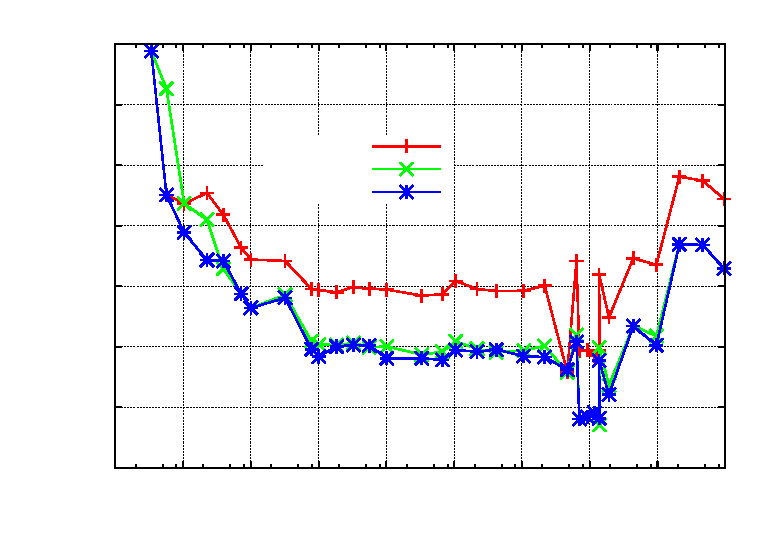
\includegraphics{../GNU/Mega168PAall}}%
    \gplfronttext
  \end{picture}%
\endgroup

\caption{Kondensator-Messfehler von drei ATmega168PA, unkalibriert}
\label{fig:mega168PAall}
\end{figure}

\begin{figure}[H]
  \begin{subfigure}[b]{9cm}
    \centering
    \resizebox{9cm}{!}{% GNUPLOT: LaTeX picture with Postscript
\begingroup
  \makeatletter
  \providecommand\color[2][]{%
    \GenericError{(gnuplot) \space\space\space\@spaces}{%
      Package color not loaded in conjunction with
      terminal option `colourtext'%
    }{See the gnuplot documentation for explanation.%
    }{Either use 'blacktext' in gnuplot or load the package
      color.sty in LaTeX.}%
    \renewcommand\color[2][]{}%
  }%
  \providecommand\includegraphics[2][]{%
    \GenericError{(gnuplot) \space\space\space\@spaces}{%
      Package graphicx or graphics not loaded%
    }{See the gnuplot documentation for explanation.%
    }{The gnuplot epslatex terminal needs graphicx.sty or graphics.sty.}%
    \renewcommand\includegraphics[2][]{}%
  }%
  \providecommand\rotatebox[2]{#2}%
  \@ifundefined{ifGPcolor}{%
    \newif\ifGPcolor
    \GPcolortrue
  }{}%
  \@ifundefined{ifGPblacktext}{%
    \newif\ifGPblacktext
    \GPblacktexttrue
  }{}%
  % define a \g@addto@macro without @ in the name:
  \let\gplgaddtomacro\g@addto@macro
  % define empty templates for all commands taking text:
  \gdef\gplbacktext{}%
  \gdef\gplfronttext{}%
  \makeatother
  \ifGPblacktext
    % no textcolor at all
    \def\colorrgb#1{}%
    \def\colorgray#1{}%
  \else
    % gray or color?
    \ifGPcolor
      \def\colorrgb#1{\color[rgb]{#1}}%
      \def\colorgray#1{\color[gray]{#1}}%
      \expandafter\def\csname LTw\endcsname{\color{white}}%
      \expandafter\def\csname LTb\endcsname{\color{black}}%
      \expandafter\def\csname LTa\endcsname{\color{black}}%
      \expandafter\def\csname LT0\endcsname{\color[rgb]{1,0,0}}%
      \expandafter\def\csname LT1\endcsname{\color[rgb]{0,1,0}}%
      \expandafter\def\csname LT2\endcsname{\color[rgb]{0,0,1}}%
      \expandafter\def\csname LT3\endcsname{\color[rgb]{1,0,1}}%
      \expandafter\def\csname LT4\endcsname{\color[rgb]{0,1,1}}%
      \expandafter\def\csname LT5\endcsname{\color[rgb]{1,1,0}}%
      \expandafter\def\csname LT6\endcsname{\color[rgb]{0,0,0}}%
      \expandafter\def\csname LT7\endcsname{\color[rgb]{1,0.3,0}}%
      \expandafter\def\csname LT8\endcsname{\color[rgb]{0.5,0.5,0.5}}%
    \else
      % gray
      \def\colorrgb#1{\color{black}}%
      \def\colorgray#1{\color[gray]{#1}}%
      \expandafter\def\csname LTw\endcsname{\color{white}}%
      \expandafter\def\csname LTb\endcsname{\color{black}}%
      \expandafter\def\csname LTa\endcsname{\color{black}}%
      \expandafter\def\csname LT0\endcsname{\color{black}}%
      \expandafter\def\csname LT1\endcsname{\color{black}}%
      \expandafter\def\csname LT2\endcsname{\color{black}}%
      \expandafter\def\csname LT3\endcsname{\color{black}}%
      \expandafter\def\csname LT4\endcsname{\color{black}}%
      \expandafter\def\csname LT5\endcsname{\color{black}}%
      \expandafter\def\csname LT6\endcsname{\color{black}}%
      \expandafter\def\csname LT7\endcsname{\color{black}}%
      \expandafter\def\csname LT8\endcsname{\color{black}}%
    \fi
  \fi
  \setlength{\unitlength}{0.0500bp}%
  \begin{picture}(7200.00,5040.00)%
    \gplgaddtomacro\gplbacktext{%
      \csname LTb\endcsname%
      \put(814,704){\makebox(0,0)[r]{\strut{}-6}}%
      \csname LTb\endcsname%
      \put(814,1156){\makebox(0,0)[r]{\strut{}-4}}%
      \csname LTb\endcsname%
      \put(814,1609){\makebox(0,0)[r]{\strut{}-2}}%
      \csname LTb\endcsname%
      \put(814,2061){\makebox(0,0)[r]{\strut{} 0}}%
      \csname LTb\endcsname%
      \put(814,2513){\makebox(0,0)[r]{\strut{} 2}}%
      \csname LTb\endcsname%
      \put(814,2966){\makebox(0,0)[r]{\strut{} 4}}%
      \csname LTb\endcsname%
      \put(814,3418){\makebox(0,0)[r]{\strut{} 6}}%
      \csname LTb\endcsname%
      \put(814,3870){\makebox(0,0)[r]{\strut{} 8}}%
      \csname LTb\endcsname%
      \put(814,4323){\makebox(0,0)[r]{\strut{} 10}}%
      \csname LTb\endcsname%
      \put(814,4775){\makebox(0,0)[r]{\strut{} 12}}%
      \csname LTb\endcsname%
      \put(946,484){\makebox(0,0){\strut{}10p}}%
      \csname LTb\endcsname%
      \put(1597,484){\makebox(0,0){\strut{}100p}}%
      \csname LTb\endcsname%
      \put(2248,484){\makebox(0,0){\strut{}1n}}%
      \csname LTb\endcsname%
      \put(2898,484){\makebox(0,0){\strut{}10n}}%
      \csname LTb\endcsname%
      \put(3549,484){\makebox(0,0){\strut{}100n}}%
      \csname LTb\endcsname%
      \put(4200,484){\makebox(0,0){\strut{}1u}}%
      \csname LTb\endcsname%
      \put(4851,484){\makebox(0,0){\strut{}10u}}%
      \csname LTb\endcsname%
      \put(5501,484){\makebox(0,0){\strut{}100u}}%
      \csname LTb\endcsname%
      \put(6152,484){\makebox(0,0){\strut{}1m}}%
      \csname LTb\endcsname%
      \put(6803,484){\makebox(0,0){\strut{}10m}}%
      \put(176,2739){\rotatebox{-270}{\makebox(0,0){\strut{}Error / Percent}}}%
      \put(3874,154){\makebox(0,0){\strut{}Capacity value / F}}%
      \put(3874,4665){\makebox(0,0){\strut{}}}%
    }%
    \gplgaddtomacro\gplfronttext{%
      \csname LTb\endcsname%
      \put(5753,4602){\makebox(0,0)[r]{\strut{}328-10}}%
      \csname LTb\endcsname%
      \put(5753,4382){\makebox(0,0)[r]{\strut{}328-11}}%
      \csname LTb\endcsname%
      \put(5753,4162){\makebox(0,0)[r]{\strut{}168-12}}%
    }%
    \gplbacktext
    \put(0,0){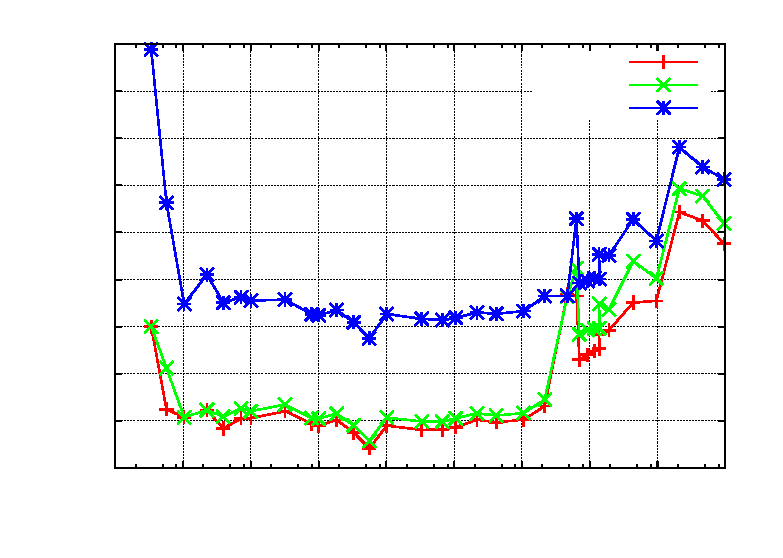
\includegraphics{../GNU/Mega328all}}%
    \gplfronttext
  \end{picture}%
\endgroup
}
    \caption{drei ATmega328}
    \label{fig:mega328all}
  \end{subfigure}
  ~
  \begin{subfigure}[b]{9cm}
    \centering
    \resizebox{9cm}{!}{% GNUPLOT: LaTeX picture with Postscript
\begingroup
  \makeatletter
  \providecommand\color[2][]{%
    \GenericError{(gnuplot) \space\space\space\@spaces}{%
      Package color not loaded in conjunction with
      terminal option `colourtext'%
    }{See the gnuplot documentation for explanation.%
    }{Either use 'blacktext' in gnuplot or load the package
      color.sty in LaTeX.}%
    \renewcommand\color[2][]{}%
  }%
  \providecommand\includegraphics[2][]{%
    \GenericError{(gnuplot) \space\space\space\@spaces}{%
      Package graphicx or graphics not loaded%
    }{See the gnuplot documentation for explanation.%
    }{The gnuplot epslatex terminal needs graphicx.sty or graphics.sty.}%
    \renewcommand\includegraphics[2][]{}%
  }%
  \providecommand\rotatebox[2]{#2}%
  \@ifundefined{ifGPcolor}{%
    \newif\ifGPcolor
    \GPcolortrue
  }{}%
  \@ifundefined{ifGPblacktext}{%
    \newif\ifGPblacktext
    \GPblacktexttrue
  }{}%
  % define a \g@addto@macro without @ in the name:
  \let\gplgaddtomacro\g@addto@macro
  % define empty templates for all commands taking text:
  \gdef\gplbacktext{}%
  \gdef\gplfronttext{}%
  \makeatother
  \ifGPblacktext
    % no textcolor at all
    \def\colorrgb#1{}%
    \def\colorgray#1{}%
  \else
    % gray or color?
    \ifGPcolor
      \def\colorrgb#1{\color[rgb]{#1}}%
      \def\colorgray#1{\color[gray]{#1}}%
      \expandafter\def\csname LTw\endcsname{\color{white}}%
      \expandafter\def\csname LTb\endcsname{\color{black}}%
      \expandafter\def\csname LTa\endcsname{\color{black}}%
      \expandafter\def\csname LT0\endcsname{\color[rgb]{1,0,0}}%
      \expandafter\def\csname LT1\endcsname{\color[rgb]{0,1,0}}%
      \expandafter\def\csname LT2\endcsname{\color[rgb]{0,0,1}}%
      \expandafter\def\csname LT3\endcsname{\color[rgb]{1,0,1}}%
      \expandafter\def\csname LT4\endcsname{\color[rgb]{0,1,1}}%
      \expandafter\def\csname LT5\endcsname{\color[rgb]{1,1,0}}%
      \expandafter\def\csname LT6\endcsname{\color[rgb]{0,0,0}}%
      \expandafter\def\csname LT7\endcsname{\color[rgb]{1,0.3,0}}%
      \expandafter\def\csname LT8\endcsname{\color[rgb]{0.5,0.5,0.5}}%
    \else
      % gray
      \def\colorrgb#1{\color{black}}%
      \def\colorgray#1{\color[gray]{#1}}%
      \expandafter\def\csname LTw\endcsname{\color{white}}%
      \expandafter\def\csname LTb\endcsname{\color{black}}%
      \expandafter\def\csname LTa\endcsname{\color{black}}%
      \expandafter\def\csname LT0\endcsname{\color{black}}%
      \expandafter\def\csname LT1\endcsname{\color{black}}%
      \expandafter\def\csname LT2\endcsname{\color{black}}%
      \expandafter\def\csname LT3\endcsname{\color{black}}%
      \expandafter\def\csname LT4\endcsname{\color{black}}%
      \expandafter\def\csname LT5\endcsname{\color{black}}%
      \expandafter\def\csname LT6\endcsname{\color{black}}%
      \expandafter\def\csname LT7\endcsname{\color{black}}%
      \expandafter\def\csname LT8\endcsname{\color{black}}%
    \fi
  \fi
  \setlength{\unitlength}{0.0500bp}%
  \begin{picture}(7200.00,5040.00)%
    \gplgaddtomacro\gplbacktext{%
      \csname LTb\endcsname%
      \put(814,704){\makebox(0,0)[r]{\strut{}-12}}%
      \csname LTb\endcsname%
      \put(814,1074){\makebox(0,0)[r]{\strut{}-10}}%
      \csname LTb\endcsname%
      \put(814,1444){\makebox(0,0)[r]{\strut{}-8}}%
      \csname LTb\endcsname%
      \put(814,1814){\makebox(0,0)[r]{\strut{}-6}}%
      \csname LTb\endcsname%
      \put(814,2184){\makebox(0,0)[r]{\strut{}-4}}%
      \csname LTb\endcsname%
      \put(814,2554){\makebox(0,0)[r]{\strut{}-2}}%
      \csname LTb\endcsname%
      \put(814,2925){\makebox(0,0)[r]{\strut{} 0}}%
      \csname LTb\endcsname%
      \put(814,3295){\makebox(0,0)[r]{\strut{} 2}}%
      \csname LTb\endcsname%
      \put(814,3665){\makebox(0,0)[r]{\strut{} 4}}%
      \csname LTb\endcsname%
      \put(814,4035){\makebox(0,0)[r]{\strut{} 6}}%
      \csname LTb\endcsname%
      \put(814,4405){\makebox(0,0)[r]{\strut{} 8}}%
      \csname LTb\endcsname%
      \put(814,4775){\makebox(0,0)[r]{\strut{} 10}}%
      \csname LTb\endcsname%
      \put(946,484){\makebox(0,0){\strut{}10p}}%
      \csname LTb\endcsname%
      \put(1597,484){\makebox(0,0){\strut{}100p}}%
      \csname LTb\endcsname%
      \put(2248,484){\makebox(0,0){\strut{}1n}}%
      \csname LTb\endcsname%
      \put(2898,484){\makebox(0,0){\strut{}10n}}%
      \csname LTb\endcsname%
      \put(3549,484){\makebox(0,0){\strut{}100n}}%
      \csname LTb\endcsname%
      \put(4200,484){\makebox(0,0){\strut{}1u}}%
      \csname LTb\endcsname%
      \put(4851,484){\makebox(0,0){\strut{}10u}}%
      \csname LTb\endcsname%
      \put(5501,484){\makebox(0,0){\strut{}100u}}%
      \csname LTb\endcsname%
      \put(6152,484){\makebox(0,0){\strut{}1m}}%
      \csname LTb\endcsname%
      \put(6803,484){\makebox(0,0){\strut{}10m}}%
      \put(176,2739){\rotatebox{-270}{\makebox(0,0){\strut{}Error / Percent}}}%
      \put(3874,154){\makebox(0,0){\strut{}Capacity value / F}}%
      \put(3874,4665){\makebox(0,0){\strut{}}}%
    }%
    \gplgaddtomacro\gplfronttext{%
      \csname LTb\endcsname%
      \put(3282,3740){\makebox(0,0)[r]{\strut{}328P-13}}%
      \csname LTb\endcsname%
      \put(3282,3520){\makebox(0,0)[r]{\strut{}328P-14}}%
      \csname LTb\endcsname%
      \put(3282,3300){\makebox(0,0)[r]{\strut{}328P-15}}%
    }%
    \gplbacktext
    \put(0,0){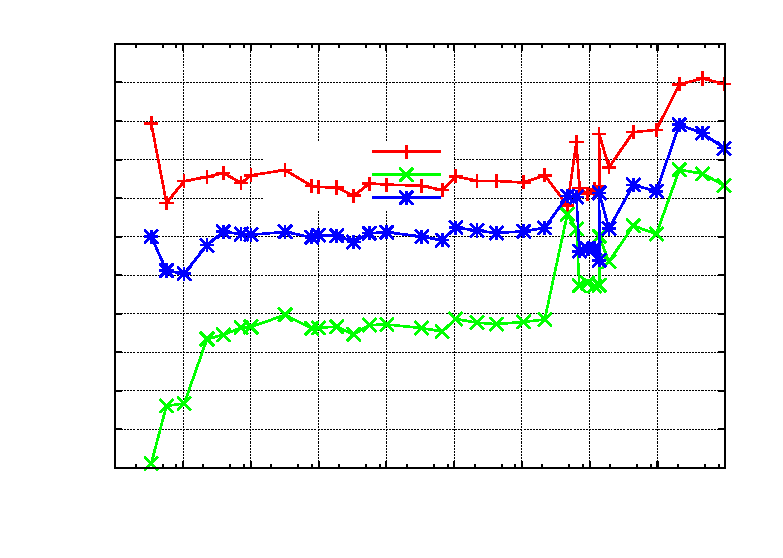
\includegraphics{../GNU/Mega328Pall}}%
    \gplfronttext
  \end{picture}%
\endgroup
}
    \caption{drei ATmega328P}
    \label{fig:mega328Pall}
  \end{subfigure}
  \caption{Kondensator-Messfehler, unkalibriert}
\end{figure}

Zum Erreichen der besten Messgenauigkeit muss die Software an die individuellen Eigenschaften des verwendeten ATmega
angepasst werden. Dazu kann die Korrekturspannung REF\_C\_KORR für den Komparator angegeben werden, der für die Messung der kleinen 
Kapazitäten eingesetzt wird. Eine Korrekturspannung von 1~mV führt zu einer Verminderung der Kapazitätsanzeige von etwa 1,1~Promille.
Bei einem automatischen Abgleich ist REF\_C\_KORR  nur ein Offset zu der gemessenen Differenzspannung von geladenem Kondensator
und der internen Referenz.
Für die großen Kapazitäten kann der Promillewert C\_H\_KORR angegeben werden, um den die Messungen
zu groß sind.
Da die großen Kondensatoren meistens Elektrolytkondensatoren mit schlechter Güte sind, ist die Bestimmung
des wahren Kapazitätswertes und damit auch des Messfehlers hier besonders schwierig.

Besonders bei den ATmega168 habe ich bei kleinen Kapazitätswerten einen Messfehler beobachtet, 
der von der Anstiegsgeschwindigkeit der Spannung beim Ladevorgang abhängig ist.
Die Abbildung~\ref{fig:mega168optcap} zeigt die Messabweichung bei Kondensatormessung nur mit der Berücksichtigung des
Nullwertes (168-3-A), mit dem Korrekturfaktor für kleine Kondensatoren REF\_C\_KORR=66 sowie dem Korrekturfaktor für große
Kondensatoren C\_H\_KORR=5 (168-3-B), sowie zusätzlich als Kurve 168-3-C  mit der Berücksichtigung einer Span\-nungs\-an\-stiegs\-kom\-po\-nen\-te 
(COMP\_SLEW1=4000 und COMP\_SLEW2=220) und des Selbst\-ent\-lade\-ver\-hal\-tens der großen Kon\-den\-sa\-toren.
Der Span\-nungs\-an\-stiegs-Kor\-rek\-tur\-faktor berechnet sich nach \(\frac{COMP\_SLEW1}{cval+COMP\_SLEW2} - \frac{COMP\_SLEW1}{COMP\_SLEW2}\),
wobei cval der gemessene Kapazitätswert in pF ist.

\begin{figure}[H]
\centering
% GNUPLOT: LaTeX picture with Postscript
\begingroup
  \makeatletter
  \providecommand\color[2][]{%
    \GenericError{(gnuplot) \space\space\space\@spaces}{%
      Package color not loaded in conjunction with
      terminal option `colourtext'%
    }{See the gnuplot documentation for explanation.%
    }{Either use 'blacktext' in gnuplot or load the package
      color.sty in LaTeX.}%
    \renewcommand\color[2][]{}%
  }%
  \providecommand\includegraphics[2][]{%
    \GenericError{(gnuplot) \space\space\space\@spaces}{%
      Package graphicx or graphics not loaded%
    }{See the gnuplot documentation for explanation.%
    }{The gnuplot epslatex terminal needs graphicx.sty or graphics.sty.}%
    \renewcommand\includegraphics[2][]{}%
  }%
  \providecommand\rotatebox[2]{#2}%
  \@ifundefined{ifGPcolor}{%
    \newif\ifGPcolor
    \GPcolortrue
  }{}%
  \@ifundefined{ifGPblacktext}{%
    \newif\ifGPblacktext
    \GPblacktexttrue
  }{}%
  % define a \g@addto@macro without @ in the name:
  \let\gplgaddtomacro\g@addto@macro
  % define empty templates for all commands taking text:
  \gdef\gplbacktext{}%
  \gdef\gplfronttext{}%
  \makeatother
  \ifGPblacktext
    % no textcolor at all
    \def\colorrgb#1{}%
    \def\colorgray#1{}%
  \else
    % gray or color?
    \ifGPcolor
      \def\colorrgb#1{\color[rgb]{#1}}%
      \def\colorgray#1{\color[gray]{#1}}%
      \expandafter\def\csname LTw\endcsname{\color{white}}%
      \expandafter\def\csname LTb\endcsname{\color{black}}%
      \expandafter\def\csname LTa\endcsname{\color{black}}%
      \expandafter\def\csname LT0\endcsname{\color[rgb]{1,0,0}}%
      \expandafter\def\csname LT1\endcsname{\color[rgb]{0,1,0}}%
      \expandafter\def\csname LT2\endcsname{\color[rgb]{0,0,1}}%
      \expandafter\def\csname LT3\endcsname{\color[rgb]{1,0,1}}%
      \expandafter\def\csname LT4\endcsname{\color[rgb]{0,1,1}}%
      \expandafter\def\csname LT5\endcsname{\color[rgb]{1,1,0}}%
      \expandafter\def\csname LT6\endcsname{\color[rgb]{0,0,0}}%
      \expandafter\def\csname LT7\endcsname{\color[rgb]{1,0.3,0}}%
      \expandafter\def\csname LT8\endcsname{\color[rgb]{0.5,0.5,0.5}}%
    \else
      % gray
      \def\colorrgb#1{\color{black}}%
      \def\colorgray#1{\color[gray]{#1}}%
      \expandafter\def\csname LTw\endcsname{\color{white}}%
      \expandafter\def\csname LTb\endcsname{\color{black}}%
      \expandafter\def\csname LTa\endcsname{\color{black}}%
      \expandafter\def\csname LT0\endcsname{\color{black}}%
      \expandafter\def\csname LT1\endcsname{\color{black}}%
      \expandafter\def\csname LT2\endcsname{\color{black}}%
      \expandafter\def\csname LT3\endcsname{\color{black}}%
      \expandafter\def\csname LT4\endcsname{\color{black}}%
      \expandafter\def\csname LT5\endcsname{\color{black}}%
      \expandafter\def\csname LT6\endcsname{\color{black}}%
      \expandafter\def\csname LT7\endcsname{\color{black}}%
      \expandafter\def\csname LT8\endcsname{\color{black}}%
    \fi
  \fi
  \setlength{\unitlength}{0.0500bp}%
  \begin{picture}(7200.00,5040.00)%
    \gplgaddtomacro\gplbacktext{%
      \csname LTb\endcsname%
      \put(814,704){\makebox(0,0)[r]{\strut{}-5}}%
      \csname LTb\endcsname%
      \put(814,1286){\makebox(0,0)[r]{\strut{} 0}}%
      \csname LTb\endcsname%
      \put(814,1867){\makebox(0,0)[r]{\strut{} 5}}%
      \csname LTb\endcsname%
      \put(814,2449){\makebox(0,0)[r]{\strut{} 10}}%
      \csname LTb\endcsname%
      \put(814,3030){\makebox(0,0)[r]{\strut{} 15}}%
      \csname LTb\endcsname%
      \put(814,3612){\makebox(0,0)[r]{\strut{} 20}}%
      \csname LTb\endcsname%
      \put(814,4193){\makebox(0,0)[r]{\strut{} 25}}%
      \csname LTb\endcsname%
      \put(814,4775){\makebox(0,0)[r]{\strut{} 30}}%
      \csname LTb\endcsname%
      \put(946,484){\makebox(0,0){\strut{}10p}}%
      \csname LTb\endcsname%
      \put(1597,484){\makebox(0,0){\strut{}100p}}%
      \csname LTb\endcsname%
      \put(2248,484){\makebox(0,0){\strut{}1n}}%
      \csname LTb\endcsname%
      \put(2898,484){\makebox(0,0){\strut{}10n}}%
      \csname LTb\endcsname%
      \put(3549,484){\makebox(0,0){\strut{}100n}}%
      \csname LTb\endcsname%
      \put(4200,484){\makebox(0,0){\strut{}1u}}%
      \csname LTb\endcsname%
      \put(4851,484){\makebox(0,0){\strut{}10u}}%
      \csname LTb\endcsname%
      \put(5501,484){\makebox(0,0){\strut{}100u}}%
      \csname LTb\endcsname%
      \put(6152,484){\makebox(0,0){\strut{}1m}}%
      \csname LTb\endcsname%
      \put(6803,484){\makebox(0,0){\strut{}10m}}%
      \put(176,2739){\rotatebox{-270}{\makebox(0,0){\strut{}Error / Percent}}}%
      \put(3874,154){\makebox(0,0){\strut{}Capacity value / F}}%
      \put(3874,4665){\makebox(0,0){\strut{}}}%
    }%
    \gplgaddtomacro\gplfronttext{%
      \csname LTb\endcsname%
      \put(5753,4602){\makebox(0,0)[r]{\strut{}168-A}}%
      \csname LTb\endcsname%
      \put(5753,4382){\makebox(0,0)[r]{\strut{}168-B}}%
      \csname LTb\endcsname%
      \put(5753,4162){\makebox(0,0)[r]{\strut{}168-C}}%
    }%
    \gplbacktext
    \put(0,0){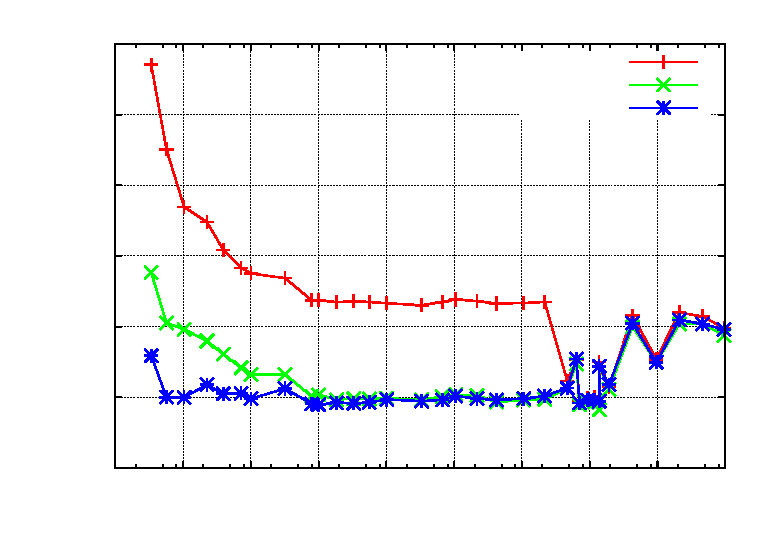
\includegraphics{../GNU/Mega168cap_opt}}%
    \gplfronttext
  \end{picture}%
\endgroup

\caption{Optimierung der Kondensator-Messung eines ATmega168}
\label{fig:mega168optcap}
\end{figure}

\subsection{Automatischer Abgleich der Kondensator-Messung}

Der automatische Abgleich besteht aus zwei Teilen. Der erste Teil besteht darin, einen Nullabgleich der Kondensatormessung durchzuführen.
Dazu wird in der Selbsttest-Routine der Mittelwert der gemessenen Kapazität bei nicht angeschlossenem Kondensator bestimmt.
Es werden die Mittelwerte aus jeweils 8 Messungen für alle 6 Messkombinationen bestimmt.
Nach erfolgreichem Abgleich werden die Korrekturwerte im EEprom festgehalten und für künftige Messungen verwendet.
Schwieriger ist die Beseitigung der Exemplarstreuungen bei der Messung von Kondensatoren bis etwa \(40 \mu F\), wie sie in den 
Abbildungen \ref{fig:mega168all}, \ref{fig:mega168Aall} und \ref{fig:mega168PAall} gezeigt wurden.
Als wesentliche Ursache wurde das unterschiedliche Verhalten (Offset-Spannung) des analogen Komparators herausgefunden.

In Abbildung \ref{fig:CompAdjust} werden die Daten von den neun untersuchten Prozessoren gezeigt.
Die Punkte ,,diff2ref'' zeigen die Spannungsdifferenz, die sich nach dem Laden eines Kondensators mit \(660 nF\) zu der
jeweiligen internen Referenzspannung ergibt. Idealerweise wäre diese Spannung immer Null, wenn der analoge
Komparator rechtzeitig das Signal zum Beenden des Ladevorganges gegeben hätte. Die kurze Verwaltungszeit des ATmega
sollte bei der relativ großen Kapazität zu keiner messbaren Spannungserhöhung geführt haben.
Die Punkte ,,CapErr'' zeigen die aus den Abbildungen \ref{fig:mega168all}, \ref{fig:mega168Aall} und \ref{fig:mega168PAall} 
geschätzten Messfehler der einzelnen ATmega-Exemplare in Promille.
Auffällig ist, wie die ,,CapErr'' Punkte den ,,diff2ref'' Punkten folgen.
Deshalb zeigen die Punkte ,,diff'' die Differenz zwischen den jeweiligen ,,CapErr'' und ,,diff2ref'' Punkten.
Mit einem mittleren Wert für diff kann man also einen guten Schätzwert für die Korrektur der Kondensatormessung aus der
Differenz der Kondensatorspannung nach dem Laden zur internen Referenzspannung berechnen.

Im zweiten Teil der Abgleichprozedur muss also ein Kondensator hoher Güte zwischen Pin~1 und Pin~3 mit einer
Kapazität zwischen \(100 nF\) und \(20 \mu F\) angeschlossen werden. 
Es sollte ein Folienkondensator, nach Möglichkeit kein keramischer Kondensator und schon gar kein
Elektrolyt-Kondensator sein. Der Kapazitätswert braucht aber für diesen Abgleich nicht genau bekannt zu sein.

\begin{figure}[H]
\centering
% GNUPLOT: LaTeX picture with Postscript
\begingroup
  \makeatletter
  \providecommand\color[2][]{%
    \GenericError{(gnuplot) \space\space\space\@spaces}{%
      Package color not loaded in conjunction with
      terminal option `colourtext'%
    }{See the gnuplot documentation for explanation.%
    }{Either use 'blacktext' in gnuplot or load the package
      color.sty in LaTeX.}%
    \renewcommand\color[2][]{}%
  }%
  \providecommand\includegraphics[2][]{%
    \GenericError{(gnuplot) \space\space\space\@spaces}{%
      Package graphicx or graphics not loaded%
    }{See the gnuplot documentation for explanation.%
    }{The gnuplot epslatex terminal needs graphicx.sty or graphics.sty.}%
    \renewcommand\includegraphics[2][]{}%
  }%
  \providecommand\rotatebox[2]{#2}%
  \@ifundefined{ifGPcolor}{%
    \newif\ifGPcolor
    \GPcolortrue
  }{}%
  \@ifundefined{ifGPblacktext}{%
    \newif\ifGPblacktext
    \GPblacktexttrue
  }{}%
  % define a \g@addto@macro without @ in the name:
  \let\gplgaddtomacro\g@addto@macro
  % define empty templates for all commands taking text:
  \gdef\gplbacktext{}%
  \gdef\gplfronttext{}%
  \makeatother
  \ifGPblacktext
    % no textcolor at all
    \def\colorrgb#1{}%
    \def\colorgray#1{}%
  \else
    % gray or color?
    \ifGPcolor
      \def\colorrgb#1{\color[rgb]{#1}}%
      \def\colorgray#1{\color[gray]{#1}}%
      \expandafter\def\csname LTw\endcsname{\color{white}}%
      \expandafter\def\csname LTb\endcsname{\color{black}}%
      \expandafter\def\csname LTa\endcsname{\color{black}}%
      \expandafter\def\csname LT0\endcsname{\color[rgb]{1,0,0}}%
      \expandafter\def\csname LT1\endcsname{\color[rgb]{0,1,0}}%
      \expandafter\def\csname LT2\endcsname{\color[rgb]{0,0,1}}%
      \expandafter\def\csname LT3\endcsname{\color[rgb]{1,0,1}}%
      \expandafter\def\csname LT4\endcsname{\color[rgb]{0,1,1}}%
      \expandafter\def\csname LT5\endcsname{\color[rgb]{1,1,0}}%
      \expandafter\def\csname LT6\endcsname{\color[rgb]{0,0,0}}%
      \expandafter\def\csname LT7\endcsname{\color[rgb]{1,0.3,0}}%
      \expandafter\def\csname LT8\endcsname{\color[rgb]{0.5,0.5,0.5}}%
    \else
      % gray
      \def\colorrgb#1{\color{black}}%
      \def\colorgray#1{\color[gray]{#1}}%
      \expandafter\def\csname LTw\endcsname{\color{white}}%
      \expandafter\def\csname LTb\endcsname{\color{black}}%
      \expandafter\def\csname LTa\endcsname{\color{black}}%
      \expandafter\def\csname LT0\endcsname{\color{black}}%
      \expandafter\def\csname LT1\endcsname{\color{black}}%
      \expandafter\def\csname LT2\endcsname{\color{black}}%
      \expandafter\def\csname LT3\endcsname{\color{black}}%
      \expandafter\def\csname LT4\endcsname{\color{black}}%
      \expandafter\def\csname LT5\endcsname{\color{black}}%
      \expandafter\def\csname LT6\endcsname{\color{black}}%
      \expandafter\def\csname LT7\endcsname{\color{black}}%
      \expandafter\def\csname LT8\endcsname{\color{black}}%
    \fi
  \fi
  \setlength{\unitlength}{0.0500bp}%
  \begin{picture}(7200.00,5040.00)%
    \gplgaddtomacro\gplbacktext{%
      \csname LTb\endcsname%
      \put(814,704){\makebox(0,0)[r]{\strut{}-20}}%
      \csname LTb\endcsname%
      \put(814,1156){\makebox(0,0)[r]{\strut{}-10}}%
      \csname LTb\endcsname%
      \put(814,1609){\makebox(0,0)[r]{\strut{} 0}}%
      \csname LTb\endcsname%
      \put(814,2061){\makebox(0,0)[r]{\strut{} 10}}%
      \csname LTb\endcsname%
      \put(814,2513){\makebox(0,0)[r]{\strut{} 20}}%
      \csname LTb\endcsname%
      \put(814,2966){\makebox(0,0)[r]{\strut{} 30}}%
      \csname LTb\endcsname%
      \put(814,3418){\makebox(0,0)[r]{\strut{} 40}}%
      \csname LTb\endcsname%
      \put(814,3870){\makebox(0,0)[r]{\strut{} 50}}%
      \csname LTb\endcsname%
      \put(814,4323){\makebox(0,0)[r]{\strut{} 60}}%
      \csname LTb\endcsname%
      \put(814,4775){\makebox(0,0)[r]{\strut{} 70}}%
      \csname LTb\endcsname%
      \put(946,484){\makebox(0,0){\strut{} 0}}%
      \csname LTb\endcsname%
      \put(2051,484){\makebox(0,0){\strut{} 2}}%
      \csname LTb\endcsname%
      \put(3157,484){\makebox(0,0){\strut{} 4}}%
      \csname LTb\endcsname%
      \put(4262,484){\makebox(0,0){\strut{} 6}}%
      \csname LTb\endcsname%
      \put(5368,484){\makebox(0,0){\strut{} 8}}%
      \csname LTb\endcsname%
      \put(6473,484){\makebox(0,0){\strut{} 10}}%
      \put(176,2739){\rotatebox{-270}{\makebox(0,0){\strut{}Error / per mill}}}%
      \put(6692,2739){\rotatebox{-270}{\makebox(0,0){\strut{}Difference to reference / mV}}}%
      \put(3709,154){\makebox(0,0){\strut{}Number of ATmega168}}%
      \put(3709,4665){\makebox(0,0){\strut{}}}%
    }%
    \gplgaddtomacro\gplfronttext{%
      \csname LTb\endcsname%
      \put(5423,4602){\makebox(0,0)[r]{\strut{}diff2ref}}%
      \csname LTb\endcsname%
      \put(5423,4382){\makebox(0,0)[r]{\strut{}CapErr}}%
      \csname LTb\endcsname%
      \put(5423,4162){\makebox(0,0)[r]{\strut{}diff}}%
    }%
    \gplbacktext
    \put(0,0){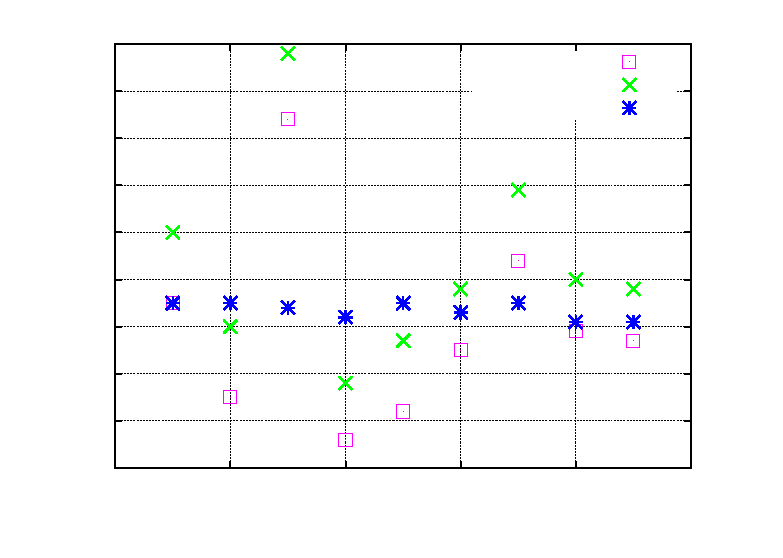
\includegraphics{../GNU/ComparatorAdjust}}%
    \gplfronttext
  \end{picture}%
\endgroup

\caption{Daten von neun ATmega168-Prozessoren}
\label{fig:CompAdjust}
\end{figure}

Die Diagramme \ref{fig:mega168cal}, \ref{fig:mega168Acal}, \ref{fig:mega168PAcal},  \ref{fig:mega328cal} und
\ref{fig:mega328Pcal} zeigen die Messergebnisse
der gleichen Prozessoren in einer Standard-Softwarekonfiguration nach der Autokalibration.
Die Prozessoren wurden alle mit der selben Software programmiert, lediglich die Makefile Option ,,PARTNO = '' musste 
wegen dem avrdude Programm an den unterschiedlichen Prozessortyp (,,m168'', ,,m168p'', ,,m328'' oder ,,m328p'') angepaßt werden.
Nach der Programmierung wurde bei jedem ATmega ein
Selbsttest gestartet und bei Test~10 ein Kondensator mit \(330 nF\) an Pin~1 und Pin~3 angeschlossen.

\begin{figure}[H]
  \begin{subfigure}[b]{9cm}
    \centering
    \resizebox{9cm}{!}{% GNUPLOT: LaTeX picture with Postscript
\begingroup
  \makeatletter
  \providecommand\color[2][]{%
    \GenericError{(gnuplot) \space\space\space\@spaces}{%
      Package color not loaded in conjunction with
      terminal option `colourtext'%
    }{See the gnuplot documentation for explanation.%
    }{Either use 'blacktext' in gnuplot or load the package
      color.sty in LaTeX.}%
    \renewcommand\color[2][]{}%
  }%
  \providecommand\includegraphics[2][]{%
    \GenericError{(gnuplot) \space\space\space\@spaces}{%
      Package graphicx or graphics not loaded%
    }{See the gnuplot documentation for explanation.%
    }{The gnuplot epslatex terminal needs graphicx.sty or graphics.sty.}%
    \renewcommand\includegraphics[2][]{}%
  }%
  \providecommand\rotatebox[2]{#2}%
  \@ifundefined{ifGPcolor}{%
    \newif\ifGPcolor
    \GPcolortrue
  }{}%
  \@ifundefined{ifGPblacktext}{%
    \newif\ifGPblacktext
    \GPblacktexttrue
  }{}%
  % define a \g@addto@macro without @ in the name:
  \let\gplgaddtomacro\g@addto@macro
  % define empty templates for all commands taking text:
  \gdef\gplbacktext{}%
  \gdef\gplfronttext{}%
  \makeatother
  \ifGPblacktext
    % no textcolor at all
    \def\colorrgb#1{}%
    \def\colorgray#1{}%
  \else
    % gray or color?
    \ifGPcolor
      \def\colorrgb#1{\color[rgb]{#1}}%
      \def\colorgray#1{\color[gray]{#1}}%
      \expandafter\def\csname LTw\endcsname{\color{white}}%
      \expandafter\def\csname LTb\endcsname{\color{black}}%
      \expandafter\def\csname LTa\endcsname{\color{black}}%
      \expandafter\def\csname LT0\endcsname{\color[rgb]{1,0,0}}%
      \expandafter\def\csname LT1\endcsname{\color[rgb]{0,1,0}}%
      \expandafter\def\csname LT2\endcsname{\color[rgb]{0,0,1}}%
      \expandafter\def\csname LT3\endcsname{\color[rgb]{1,0,1}}%
      \expandafter\def\csname LT4\endcsname{\color[rgb]{0,1,1}}%
      \expandafter\def\csname LT5\endcsname{\color[rgb]{1,1,0}}%
      \expandafter\def\csname LT6\endcsname{\color[rgb]{0,0,0}}%
      \expandafter\def\csname LT7\endcsname{\color[rgb]{1,0.3,0}}%
      \expandafter\def\csname LT8\endcsname{\color[rgb]{0.5,0.5,0.5}}%
    \else
      % gray
      \def\colorrgb#1{\color{black}}%
      \def\colorgray#1{\color[gray]{#1}}%
      \expandafter\def\csname LTw\endcsname{\color{white}}%
      \expandafter\def\csname LTb\endcsname{\color{black}}%
      \expandafter\def\csname LTa\endcsname{\color{black}}%
      \expandafter\def\csname LT0\endcsname{\color{black}}%
      \expandafter\def\csname LT1\endcsname{\color{black}}%
      \expandafter\def\csname LT2\endcsname{\color{black}}%
      \expandafter\def\csname LT3\endcsname{\color{black}}%
      \expandafter\def\csname LT4\endcsname{\color{black}}%
      \expandafter\def\csname LT5\endcsname{\color{black}}%
      \expandafter\def\csname LT6\endcsname{\color{black}}%
      \expandafter\def\csname LT7\endcsname{\color{black}}%
      \expandafter\def\csname LT8\endcsname{\color{black}}%
    \fi
  \fi
  \setlength{\unitlength}{0.0500bp}%
  \begin{picture}(7200.00,5040.00)%
    \gplgaddtomacro\gplbacktext{%
      \csname LTb\endcsname%
      \put(682,704){\makebox(0,0)[r]{\strut{}-4}}%
      \csname LTb\endcsname%
      \put(682,1074){\makebox(0,0)[r]{\strut{}-3}}%
      \csname LTb\endcsname%
      \put(682,1444){\makebox(0,0)[r]{\strut{}-2}}%
      \csname LTb\endcsname%
      \put(682,1814){\makebox(0,0)[r]{\strut{}-1}}%
      \csname LTb\endcsname%
      \put(682,2184){\makebox(0,0)[r]{\strut{} 0}}%
      \csname LTb\endcsname%
      \put(682,2554){\makebox(0,0)[r]{\strut{} 1}}%
      \csname LTb\endcsname%
      \put(682,2925){\makebox(0,0)[r]{\strut{} 2}}%
      \csname LTb\endcsname%
      \put(682,3295){\makebox(0,0)[r]{\strut{} 3}}%
      \csname LTb\endcsname%
      \put(682,3665){\makebox(0,0)[r]{\strut{} 4}}%
      \csname LTb\endcsname%
      \put(682,4035){\makebox(0,0)[r]{\strut{} 5}}%
      \csname LTb\endcsname%
      \put(682,4405){\makebox(0,0)[r]{\strut{} 6}}%
      \csname LTb\endcsname%
      \put(682,4775){\makebox(0,0)[r]{\strut{} 7}}%
      \csname LTb\endcsname%
      \put(814,484){\makebox(0,0){\strut{}10p}}%
      \csname LTb\endcsname%
      \put(1479,484){\makebox(0,0){\strut{}100p}}%
      \csname LTb\endcsname%
      \put(2145,484){\makebox(0,0){\strut{}1n}}%
      \csname LTb\endcsname%
      \put(2810,484){\makebox(0,0){\strut{}10n}}%
      \csname LTb\endcsname%
      \put(3476,484){\makebox(0,0){\strut{}100n}}%
      \csname LTb\endcsname%
      \put(4141,484){\makebox(0,0){\strut{}1u}}%
      \csname LTb\endcsname%
      \put(4807,484){\makebox(0,0){\strut{}10u}}%
      \csname LTb\endcsname%
      \put(5472,484){\makebox(0,0){\strut{}100u}}%
      \csname LTb\endcsname%
      \put(6138,484){\makebox(0,0){\strut{}1m}}%
      \csname LTb\endcsname%
      \put(6803,484){\makebox(0,0){\strut{}10m}}%
      \put(176,2739){\rotatebox{-270}{\makebox(0,0){\strut{}Error / Percent}}}%
      \put(3808,154){\makebox(0,0){\strut{}Capacity value / F}}%
      \put(3808,4665){\makebox(0,0){\strut{}}}%
    }%
    \gplgaddtomacro\gplfronttext{%
      \csname LTb\endcsname%
      \put(1606,4602){\makebox(0,0)[r]{\strut{}168-1}}%
      \csname LTb\endcsname%
      \put(1606,4382){\makebox(0,0)[r]{\strut{}168-2}}%
      \csname LTb\endcsname%
      \put(1606,4162){\makebox(0,0)[r]{\strut{}168-3}}%
    }%
    \gplbacktext
    \put(0,0){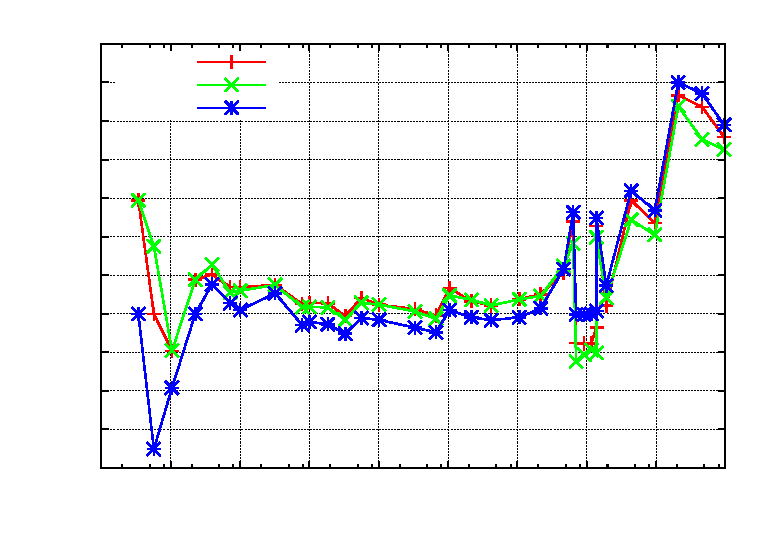
\includegraphics{../GNU/Mega168cal}}%
    \gplfronttext
  \end{picture}%
\endgroup
}
    \caption{drei ATmega168}
    \label{fig:mega168cal}
  \end{subfigure}
  ~
  \begin{subfigure}[b]{9cm}
    \centering
    \resizebox{9cm}{!}{% GNUPLOT: LaTeX picture with Postscript
\begingroup
  \makeatletter
  \providecommand\color[2][]{%
    \GenericError{(gnuplot) \space\space\space\@spaces}{%
      Package color not loaded in conjunction with
      terminal option `colourtext'%
    }{See the gnuplot documentation for explanation.%
    }{Either use 'blacktext' in gnuplot or load the package
      color.sty in LaTeX.}%
    \renewcommand\color[2][]{}%
  }%
  \providecommand\includegraphics[2][]{%
    \GenericError{(gnuplot) \space\space\space\@spaces}{%
      Package graphicx or graphics not loaded%
    }{See the gnuplot documentation for explanation.%
    }{The gnuplot epslatex terminal needs graphicx.sty or graphics.sty.}%
    \renewcommand\includegraphics[2][]{}%
  }%
  \providecommand\rotatebox[2]{#2}%
  \@ifundefined{ifGPcolor}{%
    \newif\ifGPcolor
    \GPcolortrue
  }{}%
  \@ifundefined{ifGPblacktext}{%
    \newif\ifGPblacktext
    \GPblacktexttrue
  }{}%
  % define a \g@addto@macro without @ in the name:
  \let\gplgaddtomacro\g@addto@macro
  % define empty templates for all commands taking text:
  \gdef\gplbacktext{}%
  \gdef\gplfronttext{}%
  \makeatother
  \ifGPblacktext
    % no textcolor at all
    \def\colorrgb#1{}%
    \def\colorgray#1{}%
  \else
    % gray or color?
    \ifGPcolor
      \def\colorrgb#1{\color[rgb]{#1}}%
      \def\colorgray#1{\color[gray]{#1}}%
      \expandafter\def\csname LTw\endcsname{\color{white}}%
      \expandafter\def\csname LTb\endcsname{\color{black}}%
      \expandafter\def\csname LTa\endcsname{\color{black}}%
      \expandafter\def\csname LT0\endcsname{\color[rgb]{1,0,0}}%
      \expandafter\def\csname LT1\endcsname{\color[rgb]{0,1,0}}%
      \expandafter\def\csname LT2\endcsname{\color[rgb]{0,0,1}}%
      \expandafter\def\csname LT3\endcsname{\color[rgb]{1,0,1}}%
      \expandafter\def\csname LT4\endcsname{\color[rgb]{0,1,1}}%
      \expandafter\def\csname LT5\endcsname{\color[rgb]{1,1,0}}%
      \expandafter\def\csname LT6\endcsname{\color[rgb]{0,0,0}}%
      \expandafter\def\csname LT7\endcsname{\color[rgb]{1,0.3,0}}%
      \expandafter\def\csname LT8\endcsname{\color[rgb]{0.5,0.5,0.5}}%
    \else
      % gray
      \def\colorrgb#1{\color{black}}%
      \def\colorgray#1{\color[gray]{#1}}%
      \expandafter\def\csname LTw\endcsname{\color{white}}%
      \expandafter\def\csname LTb\endcsname{\color{black}}%
      \expandafter\def\csname LTa\endcsname{\color{black}}%
      \expandafter\def\csname LT0\endcsname{\color{black}}%
      \expandafter\def\csname LT1\endcsname{\color{black}}%
      \expandafter\def\csname LT2\endcsname{\color{black}}%
      \expandafter\def\csname LT3\endcsname{\color{black}}%
      \expandafter\def\csname LT4\endcsname{\color{black}}%
      \expandafter\def\csname LT5\endcsname{\color{black}}%
      \expandafter\def\csname LT6\endcsname{\color{black}}%
      \expandafter\def\csname LT7\endcsname{\color{black}}%
      \expandafter\def\csname LT8\endcsname{\color{black}}%
    \fi
  \fi
  \setlength{\unitlength}{0.0500bp}%
  \begin{picture}(7200.00,5040.00)%
    \gplgaddtomacro\gplbacktext{%
      \csname LTb\endcsname%
      \put(682,704){\makebox(0,0)[r]{\strut{}-4}}%
      \csname LTb\endcsname%
      \put(682,1111){\makebox(0,0)[r]{\strut{}-3}}%
      \csname LTb\endcsname%
      \put(682,1518){\makebox(0,0)[r]{\strut{}-2}}%
      \csname LTb\endcsname%
      \put(682,1925){\makebox(0,0)[r]{\strut{}-1}}%
      \csname LTb\endcsname%
      \put(682,2332){\makebox(0,0)[r]{\strut{} 0}}%
      \csname LTb\endcsname%
      \put(682,2740){\makebox(0,0)[r]{\strut{} 1}}%
      \csname LTb\endcsname%
      \put(682,3147){\makebox(0,0)[r]{\strut{} 2}}%
      \csname LTb\endcsname%
      \put(682,3554){\makebox(0,0)[r]{\strut{} 3}}%
      \csname LTb\endcsname%
      \put(682,3961){\makebox(0,0)[r]{\strut{} 4}}%
      \csname LTb\endcsname%
      \put(682,4368){\makebox(0,0)[r]{\strut{} 5}}%
      \csname LTb\endcsname%
      \put(682,4775){\makebox(0,0)[r]{\strut{} 6}}%
      \csname LTb\endcsname%
      \put(814,484){\makebox(0,0){\strut{}10p}}%
      \csname LTb\endcsname%
      \put(1479,484){\makebox(0,0){\strut{}100p}}%
      \csname LTb\endcsname%
      \put(2145,484){\makebox(0,0){\strut{}1n}}%
      \csname LTb\endcsname%
      \put(2810,484){\makebox(0,0){\strut{}10n}}%
      \csname LTb\endcsname%
      \put(3476,484){\makebox(0,0){\strut{}100n}}%
      \csname LTb\endcsname%
      \put(4141,484){\makebox(0,0){\strut{}1u}}%
      \csname LTb\endcsname%
      \put(4807,484){\makebox(0,0){\strut{}10u}}%
      \csname LTb\endcsname%
      \put(5472,484){\makebox(0,0){\strut{}100u}}%
      \csname LTb\endcsname%
      \put(6138,484){\makebox(0,0){\strut{}1m}}%
      \csname LTb\endcsname%
      \put(6803,484){\makebox(0,0){\strut{}10m}}%
      \put(176,2739){\rotatebox{-270}{\makebox(0,0){\strut{}Error / Percent}}}%
      \put(3808,154){\makebox(0,0){\strut{}Capacity value / F}}%
      \put(3808,4665){\makebox(0,0){\strut{}}}%
    }%
    \gplgaddtomacro\gplfronttext{%
      \csname LTb\endcsname%
      \put(1738,4602){\makebox(0,0)[r]{\strut{}168A-4}}%
      \csname LTb\endcsname%
      \put(1738,4382){\makebox(0,0)[r]{\strut{}168A-5}}%
      \csname LTb\endcsname%
      \put(1738,4162){\makebox(0,0)[r]{\strut{}168A-6}}%
    }%
    \gplbacktext
    \put(0,0){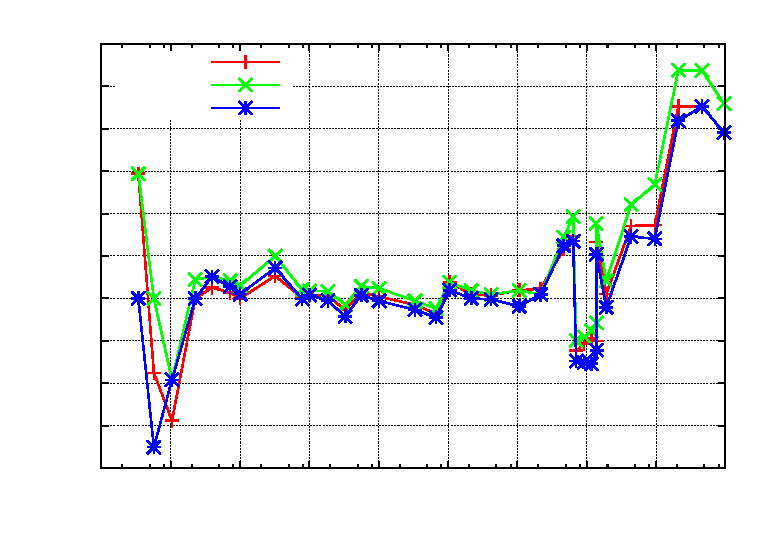
\includegraphics{../GNU/Mega168Acal}}%
    \gplfronttext
  \end{picture}%
\endgroup
}
    \caption{drei ATmega168A}
    \label{fig:mega168Acal}
  \end{subfigure}
  \caption{Kondensator-Messfehler, kalibriert}
\end{figure}

\begin{figure}[H]
\centering
% GNUPLOT: LaTeX picture with Postscript
\begingroup
  \makeatletter
  \providecommand\color[2][]{%
    \GenericError{(gnuplot) \space\space\space\@spaces}{%
      Package color not loaded in conjunction with
      terminal option `colourtext'%
    }{See the gnuplot documentation for explanation.%
    }{Either use 'blacktext' in gnuplot or load the package
      color.sty in LaTeX.}%
    \renewcommand\color[2][]{}%
  }%
  \providecommand\includegraphics[2][]{%
    \GenericError{(gnuplot) \space\space\space\@spaces}{%
      Package graphicx or graphics not loaded%
    }{See the gnuplot documentation for explanation.%
    }{The gnuplot epslatex terminal needs graphicx.sty or graphics.sty.}%
    \renewcommand\includegraphics[2][]{}%
  }%
  \providecommand\rotatebox[2]{#2}%
  \@ifundefined{ifGPcolor}{%
    \newif\ifGPcolor
    \GPcolortrue
  }{}%
  \@ifundefined{ifGPblacktext}{%
    \newif\ifGPblacktext
    \GPblacktexttrue
  }{}%
  % define a \g@addto@macro without @ in the name:
  \let\gplgaddtomacro\g@addto@macro
  % define empty templates for all commands taking text:
  \gdef\gplbacktext{}%
  \gdef\gplfronttext{}%
  \makeatother
  \ifGPblacktext
    % no textcolor at all
    \def\colorrgb#1{}%
    \def\colorgray#1{}%
  \else
    % gray or color?
    \ifGPcolor
      \def\colorrgb#1{\color[rgb]{#1}}%
      \def\colorgray#1{\color[gray]{#1}}%
      \expandafter\def\csname LTw\endcsname{\color{white}}%
      \expandafter\def\csname LTb\endcsname{\color{black}}%
      \expandafter\def\csname LTa\endcsname{\color{black}}%
      \expandafter\def\csname LT0\endcsname{\color[rgb]{1,0,0}}%
      \expandafter\def\csname LT1\endcsname{\color[rgb]{0,1,0}}%
      \expandafter\def\csname LT2\endcsname{\color[rgb]{0,0,1}}%
      \expandafter\def\csname LT3\endcsname{\color[rgb]{1,0,1}}%
      \expandafter\def\csname LT4\endcsname{\color[rgb]{0,1,1}}%
      \expandafter\def\csname LT5\endcsname{\color[rgb]{1,1,0}}%
      \expandafter\def\csname LT6\endcsname{\color[rgb]{0,0,0}}%
      \expandafter\def\csname LT7\endcsname{\color[rgb]{1,0.3,0}}%
      \expandafter\def\csname LT8\endcsname{\color[rgb]{0.5,0.5,0.5}}%
    \else
      % gray
      \def\colorrgb#1{\color{black}}%
      \def\colorgray#1{\color[gray]{#1}}%
      \expandafter\def\csname LTw\endcsname{\color{white}}%
      \expandafter\def\csname LTb\endcsname{\color{black}}%
      \expandafter\def\csname LTa\endcsname{\color{black}}%
      \expandafter\def\csname LT0\endcsname{\color{black}}%
      \expandafter\def\csname LT1\endcsname{\color{black}}%
      \expandafter\def\csname LT2\endcsname{\color{black}}%
      \expandafter\def\csname LT3\endcsname{\color{black}}%
      \expandafter\def\csname LT4\endcsname{\color{black}}%
      \expandafter\def\csname LT5\endcsname{\color{black}}%
      \expandafter\def\csname LT6\endcsname{\color{black}}%
      \expandafter\def\csname LT7\endcsname{\color{black}}%
      \expandafter\def\csname LT8\endcsname{\color{black}}%
    \fi
  \fi
  \setlength{\unitlength}{0.0500bp}%
  \begin{picture}(7200.00,5040.00)%
    \gplgaddtomacro\gplbacktext{%
      \csname LTb\endcsname%
      \put(682,704){\makebox(0,0)[r]{\strut{}-4}}%
      \csname LTb\endcsname%
      \put(682,1383){\makebox(0,0)[r]{\strut{}-2}}%
      \csname LTb\endcsname%
      \put(682,2061){\makebox(0,0)[r]{\strut{} 0}}%
      \csname LTb\endcsname%
      \put(682,2740){\makebox(0,0)[r]{\strut{} 2}}%
      \csname LTb\endcsname%
      \put(682,3418){\makebox(0,0)[r]{\strut{} 4}}%
      \csname LTb\endcsname%
      \put(682,4097){\makebox(0,0)[r]{\strut{} 6}}%
      \csname LTb\endcsname%
      \put(682,4775){\makebox(0,0)[r]{\strut{} 8}}%
      \csname LTb\endcsname%
      \put(814,484){\makebox(0,0){\strut{}10p}}%
      \csname LTb\endcsname%
      \put(1479,484){\makebox(0,0){\strut{}100p}}%
      \csname LTb\endcsname%
      \put(2145,484){\makebox(0,0){\strut{}1n}}%
      \csname LTb\endcsname%
      \put(2810,484){\makebox(0,0){\strut{}10n}}%
      \csname LTb\endcsname%
      \put(3476,484){\makebox(0,0){\strut{}100n}}%
      \csname LTb\endcsname%
      \put(4141,484){\makebox(0,0){\strut{}1u}}%
      \csname LTb\endcsname%
      \put(4807,484){\makebox(0,0){\strut{}10u}}%
      \csname LTb\endcsname%
      \put(5472,484){\makebox(0,0){\strut{}100u}}%
      \csname LTb\endcsname%
      \put(6138,484){\makebox(0,0){\strut{}1m}}%
      \csname LTb\endcsname%
      \put(6803,484){\makebox(0,0){\strut{}10m}}%
      \put(176,2739){\rotatebox{-270}{\makebox(0,0){\strut{}Error / Percent}}}%
      \put(3808,154){\makebox(0,0){\strut{}Capacity value / F}}%
      \put(3808,4665){\makebox(0,0){\strut{}}}%
    }%
    \gplgaddtomacro\gplfronttext{%
      \csname LTb\endcsname%
      \put(1870,4602){\makebox(0,0)[r]{\strut{}168PA-7}}%
      \csname LTb\endcsname%
      \put(1870,4382){\makebox(0,0)[r]{\strut{}168PA-8}}%
      \csname LTb\endcsname%
      \put(1870,4162){\makebox(0,0)[r]{\strut{}168PA-9}}%
    }%
    \gplbacktext
    \put(0,0){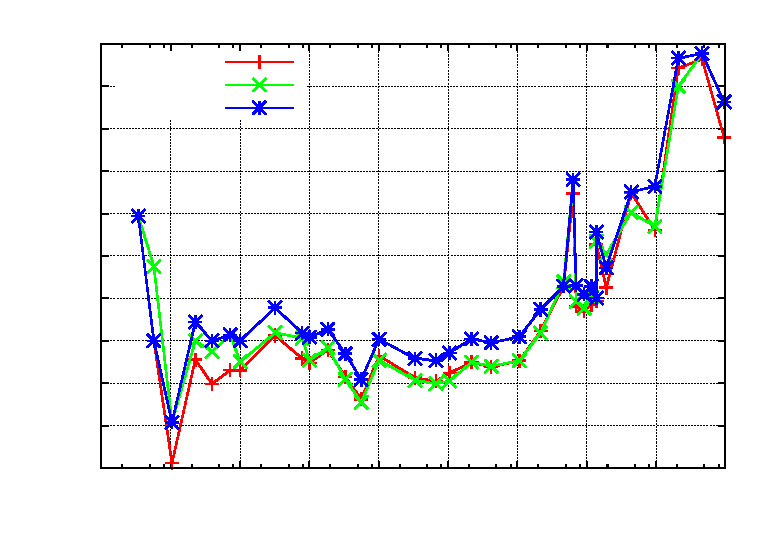
\includegraphics{../GNU/Mega168PAcal}}%
    \gplfronttext
  \end{picture}%
\endgroup

\caption{Kondensator-Messfehler von drei ATmega168PA, kalibriert}
\label{fig:mega168PAcal}
\end{figure}

\begin{figure}[H]
  \begin{subfigure}[b]{9cm}
    \centering
    \resizebox{9cm}{!}{% GNUPLOT: LaTeX picture with Postscript
\begingroup
  \makeatletter
  \providecommand\color[2][]{%
    \GenericError{(gnuplot) \space\space\space\@spaces}{%
      Package color not loaded in conjunction with
      terminal option `colourtext'%
    }{See the gnuplot documentation for explanation.%
    }{Either use 'blacktext' in gnuplot or load the package
      color.sty in LaTeX.}%
    \renewcommand\color[2][]{}%
  }%
  \providecommand\includegraphics[2][]{%
    \GenericError{(gnuplot) \space\space\space\@spaces}{%
      Package graphicx or graphics not loaded%
    }{See the gnuplot documentation for explanation.%
    }{The gnuplot epslatex terminal needs graphicx.sty or graphics.sty.}%
    \renewcommand\includegraphics[2][]{}%
  }%
  \providecommand\rotatebox[2]{#2}%
  \@ifundefined{ifGPcolor}{%
    \newif\ifGPcolor
    \GPcolortrue
  }{}%
  \@ifundefined{ifGPblacktext}{%
    \newif\ifGPblacktext
    \GPblacktexttrue
  }{}%
  % define a \g@addto@macro without @ in the name:
  \let\gplgaddtomacro\g@addto@macro
  % define empty templates for all commands taking text:
  \gdef\gplbacktext{}%
  \gdef\gplfronttext{}%
  \makeatother
  \ifGPblacktext
    % no textcolor at all
    \def\colorrgb#1{}%
    \def\colorgray#1{}%
  \else
    % gray or color?
    \ifGPcolor
      \def\colorrgb#1{\color[rgb]{#1}}%
      \def\colorgray#1{\color[gray]{#1}}%
      \expandafter\def\csname LTw\endcsname{\color{white}}%
      \expandafter\def\csname LTb\endcsname{\color{black}}%
      \expandafter\def\csname LTa\endcsname{\color{black}}%
      \expandafter\def\csname LT0\endcsname{\color[rgb]{1,0,0}}%
      \expandafter\def\csname LT1\endcsname{\color[rgb]{0,1,0}}%
      \expandafter\def\csname LT2\endcsname{\color[rgb]{0,0,1}}%
      \expandafter\def\csname LT3\endcsname{\color[rgb]{1,0,1}}%
      \expandafter\def\csname LT4\endcsname{\color[rgb]{0,1,1}}%
      \expandafter\def\csname LT5\endcsname{\color[rgb]{1,1,0}}%
      \expandafter\def\csname LT6\endcsname{\color[rgb]{0,0,0}}%
      \expandafter\def\csname LT7\endcsname{\color[rgb]{1,0.3,0}}%
      \expandafter\def\csname LT8\endcsname{\color[rgb]{0.5,0.5,0.5}}%
    \else
      % gray
      \def\colorrgb#1{\color{black}}%
      \def\colorgray#1{\color[gray]{#1}}%
      \expandafter\def\csname LTw\endcsname{\color{white}}%
      \expandafter\def\csname LTb\endcsname{\color{black}}%
      \expandafter\def\csname LTa\endcsname{\color{black}}%
      \expandafter\def\csname LT0\endcsname{\color{black}}%
      \expandafter\def\csname LT1\endcsname{\color{black}}%
      \expandafter\def\csname LT2\endcsname{\color{black}}%
      \expandafter\def\csname LT3\endcsname{\color{black}}%
      \expandafter\def\csname LT4\endcsname{\color{black}}%
      \expandafter\def\csname LT5\endcsname{\color{black}}%
      \expandafter\def\csname LT6\endcsname{\color{black}}%
      \expandafter\def\csname LT7\endcsname{\color{black}}%
      \expandafter\def\csname LT8\endcsname{\color{black}}%
    \fi
  \fi
  \setlength{\unitlength}{0.0500bp}%
  \begin{picture}(7200.00,5040.00)%
    \gplgaddtomacro\gplbacktext{%
      \csname LTb\endcsname%
      \put(682,704){\makebox(0,0)[r]{\strut{}-2}}%
      \csname LTb\endcsname%
      \put(682,1111){\makebox(0,0)[r]{\strut{}-1}}%
      \csname LTb\endcsname%
      \put(682,1518){\makebox(0,0)[r]{\strut{} 0}}%
      \csname LTb\endcsname%
      \put(682,1925){\makebox(0,0)[r]{\strut{} 1}}%
      \csname LTb\endcsname%
      \put(682,2332){\makebox(0,0)[r]{\strut{} 2}}%
      \csname LTb\endcsname%
      \put(682,2740){\makebox(0,0)[r]{\strut{} 3}}%
      \csname LTb\endcsname%
      \put(682,3147){\makebox(0,0)[r]{\strut{} 4}}%
      \csname LTb\endcsname%
      \put(682,3554){\makebox(0,0)[r]{\strut{} 5}}%
      \csname LTb\endcsname%
      \put(682,3961){\makebox(0,0)[r]{\strut{} 6}}%
      \csname LTb\endcsname%
      \put(682,4368){\makebox(0,0)[r]{\strut{} 7}}%
      \csname LTb\endcsname%
      \put(682,4775){\makebox(0,0)[r]{\strut{} 8}}%
      \csname LTb\endcsname%
      \put(814,484){\makebox(0,0){\strut{}10p}}%
      \csname LTb\endcsname%
      \put(1479,484){\makebox(0,0){\strut{}100p}}%
      \csname LTb\endcsname%
      \put(2145,484){\makebox(0,0){\strut{}1n}}%
      \csname LTb\endcsname%
      \put(2810,484){\makebox(0,0){\strut{}10n}}%
      \csname LTb\endcsname%
      \put(3476,484){\makebox(0,0){\strut{}100n}}%
      \csname LTb\endcsname%
      \put(4141,484){\makebox(0,0){\strut{}1u}}%
      \csname LTb\endcsname%
      \put(4807,484){\makebox(0,0){\strut{}10u}}%
      \csname LTb\endcsname%
      \put(5472,484){\makebox(0,0){\strut{}100u}}%
      \csname LTb\endcsname%
      \put(6138,484){\makebox(0,0){\strut{}1m}}%
      \csname LTb\endcsname%
      \put(6803,484){\makebox(0,0){\strut{}10m}}%
      \put(176,2739){\rotatebox{-270}{\makebox(0,0){\strut{}Error / Percent}}}%
      \put(3808,154){\makebox(0,0){\strut{}Capacity value / F}}%
      \put(3808,4665){\makebox(0,0){\strut{}}}%
    }%
    \gplgaddtomacro\gplfronttext{%
      \csname LTb\endcsname%
      \put(1738,4602){\makebox(0,0)[r]{\strut{}328-10}}%
      \csname LTb\endcsname%
      \put(1738,4382){\makebox(0,0)[r]{\strut{}328-11}}%
      \csname LTb\endcsname%
      \put(1738,4162){\makebox(0,0)[r]{\strut{}328-12}}%
    }%
    \gplbacktext
    \put(0,0){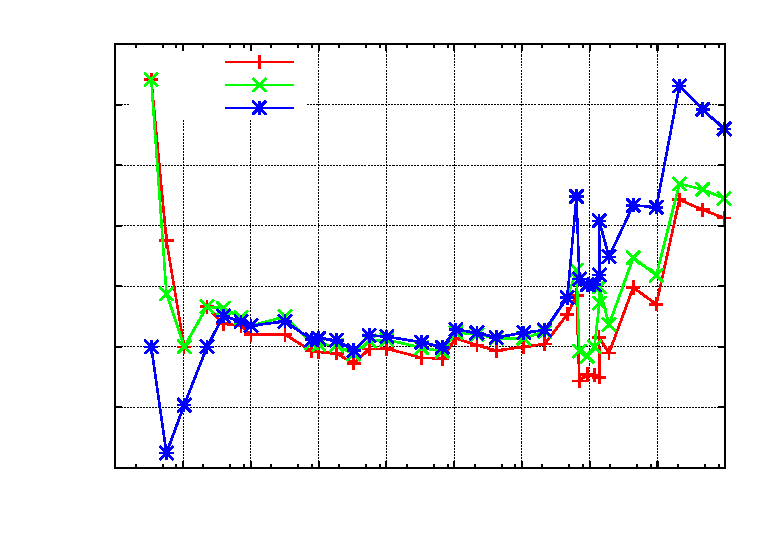
\includegraphics{../GNU/Mega328cal}}%
    \gplfronttext
  \end{picture}%
\endgroup
}
    \caption{drei ATmega328}
    \label{fig:mega328cal}
  \end{subfigure}
  ~
  \begin{subfigure}[b]{9cm}
    \centering
    \resizebox{9cm}{!}{% GNUPLOT: LaTeX picture with Postscript
\begingroup
  \makeatletter
  \providecommand\color[2][]{%
    \GenericError{(gnuplot) \space\space\space\@spaces}{%
      Package color not loaded in conjunction with
      terminal option `colourtext'%
    }{See the gnuplot documentation for explanation.%
    }{Either use 'blacktext' in gnuplot or load the package
      color.sty in LaTeX.}%
    \renewcommand\color[2][]{}%
  }%
  \providecommand\includegraphics[2][]{%
    \GenericError{(gnuplot) \space\space\space\@spaces}{%
      Package graphicx or graphics not loaded%
    }{See the gnuplot documentation for explanation.%
    }{The gnuplot epslatex terminal needs graphicx.sty or graphics.sty.}%
    \renewcommand\includegraphics[2][]{}%
  }%
  \providecommand\rotatebox[2]{#2}%
  \@ifundefined{ifGPcolor}{%
    \newif\ifGPcolor
    \GPcolortrue
  }{}%
  \@ifundefined{ifGPblacktext}{%
    \newif\ifGPblacktext
    \GPblacktexttrue
  }{}%
  % define a \g@addto@macro without @ in the name:
  \let\gplgaddtomacro\g@addto@macro
  % define empty templates for all commands taking text:
  \gdef\gplbacktext{}%
  \gdef\gplfronttext{}%
  \makeatother
  \ifGPblacktext
    % no textcolor at all
    \def\colorrgb#1{}%
    \def\colorgray#1{}%
  \else
    % gray or color?
    \ifGPcolor
      \def\colorrgb#1{\color[rgb]{#1}}%
      \def\colorgray#1{\color[gray]{#1}}%
      \expandafter\def\csname LTw\endcsname{\color{white}}%
      \expandafter\def\csname LTb\endcsname{\color{black}}%
      \expandafter\def\csname LTa\endcsname{\color{black}}%
      \expandafter\def\csname LT0\endcsname{\color[rgb]{1,0,0}}%
      \expandafter\def\csname LT1\endcsname{\color[rgb]{0,1,0}}%
      \expandafter\def\csname LT2\endcsname{\color[rgb]{0,0,1}}%
      \expandafter\def\csname LT3\endcsname{\color[rgb]{1,0,1}}%
      \expandafter\def\csname LT4\endcsname{\color[rgb]{0,1,1}}%
      \expandafter\def\csname LT5\endcsname{\color[rgb]{1,1,0}}%
      \expandafter\def\csname LT6\endcsname{\color[rgb]{0,0,0}}%
      \expandafter\def\csname LT7\endcsname{\color[rgb]{1,0.3,0}}%
      \expandafter\def\csname LT8\endcsname{\color[rgb]{0.5,0.5,0.5}}%
    \else
      % gray
      \def\colorrgb#1{\color{black}}%
      \def\colorgray#1{\color[gray]{#1}}%
      \expandafter\def\csname LTw\endcsname{\color{white}}%
      \expandafter\def\csname LTb\endcsname{\color{black}}%
      \expandafter\def\csname LTa\endcsname{\color{black}}%
      \expandafter\def\csname LT0\endcsname{\color{black}}%
      \expandafter\def\csname LT1\endcsname{\color{black}}%
      \expandafter\def\csname LT2\endcsname{\color{black}}%
      \expandafter\def\csname LT3\endcsname{\color{black}}%
      \expandafter\def\csname LT4\endcsname{\color{black}}%
      \expandafter\def\csname LT5\endcsname{\color{black}}%
      \expandafter\def\csname LT6\endcsname{\color{black}}%
      \expandafter\def\csname LT7\endcsname{\color{black}}%
      \expandafter\def\csname LT8\endcsname{\color{black}}%
    \fi
  \fi
  \setlength{\unitlength}{0.0500bp}%
  \begin{picture}(7200.00,5040.00)%
    \gplgaddtomacro\gplbacktext{%
      \csname LTb\endcsname%
      \put(682,704){\makebox(0,0)[r]{\strut{}-4}}%
      \csname LTb\endcsname%
      \put(682,1383){\makebox(0,0)[r]{\strut{}-2}}%
      \csname LTb\endcsname%
      \put(682,2061){\makebox(0,0)[r]{\strut{} 0}}%
      \csname LTb\endcsname%
      \put(682,2740){\makebox(0,0)[r]{\strut{} 2}}%
      \csname LTb\endcsname%
      \put(682,3418){\makebox(0,0)[r]{\strut{} 4}}%
      \csname LTb\endcsname%
      \put(682,4097){\makebox(0,0)[r]{\strut{} 6}}%
      \csname LTb\endcsname%
      \put(682,4775){\makebox(0,0)[r]{\strut{} 8}}%
      \csname LTb\endcsname%
      \put(814,484){\makebox(0,0){\strut{}10p}}%
      \csname LTb\endcsname%
      \put(1479,484){\makebox(0,0){\strut{}100p}}%
      \csname LTb\endcsname%
      \put(2145,484){\makebox(0,0){\strut{}1n}}%
      \csname LTb\endcsname%
      \put(2810,484){\makebox(0,0){\strut{}10n}}%
      \csname LTb\endcsname%
      \put(3476,484){\makebox(0,0){\strut{}100n}}%
      \csname LTb\endcsname%
      \put(4141,484){\makebox(0,0){\strut{}1u}}%
      \csname LTb\endcsname%
      \put(4807,484){\makebox(0,0){\strut{}10u}}%
      \csname LTb\endcsname%
      \put(5472,484){\makebox(0,0){\strut{}100u}}%
      \csname LTb\endcsname%
      \put(6138,484){\makebox(0,0){\strut{}1m}}%
      \csname LTb\endcsname%
      \put(6803,484){\makebox(0,0){\strut{}10m}}%
      \put(176,2739){\rotatebox{-270}{\makebox(0,0){\strut{}Error / Percent}}}%
      \put(3808,154){\makebox(0,0){\strut{}Capacity value / F}}%
      \put(3808,4665){\makebox(0,0){\strut{}}}%
    }%
    \gplgaddtomacro\gplfronttext{%
      \csname LTb\endcsname%
      \put(1870,4602){\makebox(0,0)[r]{\strut{}328P-13}}%
      \csname LTb\endcsname%
      \put(1870,4382){\makebox(0,0)[r]{\strut{}328P-14}}%
      \csname LTb\endcsname%
      \put(1870,4162){\makebox(0,0)[r]{\strut{}328P-15}}%
    }%
    \gplbacktext
    \put(0,0){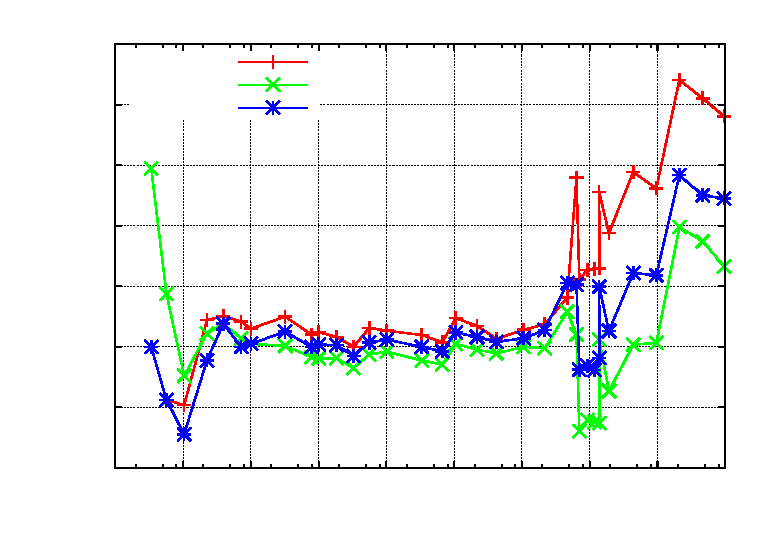
\includegraphics{../GNU/Mega328Pcal}}%
    \gplfronttext
  \end{picture}%
\endgroup
}
    \caption{drei ATmega328P}
    \label{fig:mega328Pcal}
  \end{subfigure}
  \caption{Kondensator-Messfehler, kalibriert}
\end{figure}

Zuletzt will ich die Wirkung der AUTO\_CAL Option im Selbstest noch einmal verdeutlichen.
Die folgende Diagramm \ref{fig:MegaAuto} zeigt die Ergebnisse von drei ATmega Prozessoren 
mit der grössten Messabweichung noch einmal vor und nach der Kalibration.
Die Punkte mit der Endung ,,unc'' zeigen die Messabweichungen ohne Kalibration.
Die Linien mit der Endung ,,cal'' zeigen die Messabweichungen der gleichen Prozessoren
mit der gleichen Software nach der Kalibration im Selbsttest-Zweig.
Die Ursache der Messabweichungen für große Kondensatoren (\textgreater\(40 \mu F\)) ist
noch nicht bekannt. Alle verwendeten Kondensatoren für diese Messreihe waren
Folienkondensatoren oder keramische Kondensatoren (\(56 pF\), \(100 pF\) und \(3,3 nF\)), keine Elkos.

\begin{figure}[H]
\centering
% GNUPLOT: LaTeX picture with Postscript
\begingroup
  \makeatletter
  \providecommand\color[2][]{%
    \GenericError{(gnuplot) \space\space\space\@spaces}{%
      Package color not loaded in conjunction with
      terminal option `colourtext'%
    }{See the gnuplot documentation for explanation.%
    }{Either use 'blacktext' in gnuplot or load the package
      color.sty in LaTeX.}%
    \renewcommand\color[2][]{}%
  }%
  \providecommand\includegraphics[2][]{%
    \GenericError{(gnuplot) \space\space\space\@spaces}{%
      Package graphicx or graphics not loaded%
    }{See the gnuplot documentation for explanation.%
    }{The gnuplot epslatex terminal needs graphicx.sty or graphics.sty.}%
    \renewcommand\includegraphics[2][]{}%
  }%
  \providecommand\rotatebox[2]{#2}%
  \@ifundefined{ifGPcolor}{%
    \newif\ifGPcolor
    \GPcolortrue
  }{}%
  \@ifundefined{ifGPblacktext}{%
    \newif\ifGPblacktext
    \GPblacktexttrue
  }{}%
  % define a \g@addto@macro without @ in the name:
  \let\gplgaddtomacro\g@addto@macro
  % define empty templates for all commands taking text:
  \gdef\gplbacktext{}%
  \gdef\gplfronttext{}%
  \makeatother
  \ifGPblacktext
    % no textcolor at all
    \def\colorrgb#1{}%
    \def\colorgray#1{}%
  \else
    % gray or color?
    \ifGPcolor
      \def\colorrgb#1{\color[rgb]{#1}}%
      \def\colorgray#1{\color[gray]{#1}}%
      \expandafter\def\csname LTw\endcsname{\color{white}}%
      \expandafter\def\csname LTb\endcsname{\color{black}}%
      \expandafter\def\csname LTa\endcsname{\color{black}}%
      \expandafter\def\csname LT0\endcsname{\color[rgb]{1,0,0}}%
      \expandafter\def\csname LT1\endcsname{\color[rgb]{0,1,0}}%
      \expandafter\def\csname LT2\endcsname{\color[rgb]{0,0,1}}%
      \expandafter\def\csname LT3\endcsname{\color[rgb]{1,0,1}}%
      \expandafter\def\csname LT4\endcsname{\color[rgb]{0,1,1}}%
      \expandafter\def\csname LT5\endcsname{\color[rgb]{1,1,0}}%
      \expandafter\def\csname LT6\endcsname{\color[rgb]{0,0,0}}%
      \expandafter\def\csname LT7\endcsname{\color[rgb]{1,0.3,0}}%
      \expandafter\def\csname LT8\endcsname{\color[rgb]{0.5,0.5,0.5}}%
    \else
      % gray
      \def\colorrgb#1{\color{black}}%
      \def\colorgray#1{\color[gray]{#1}}%
      \expandafter\def\csname LTw\endcsname{\color{white}}%
      \expandafter\def\csname LTb\endcsname{\color{black}}%
      \expandafter\def\csname LTa\endcsname{\color{black}}%
      \expandafter\def\csname LT0\endcsname{\color{black}}%
      \expandafter\def\csname LT1\endcsname{\color{black}}%
      \expandafter\def\csname LT2\endcsname{\color{black}}%
      \expandafter\def\csname LT3\endcsname{\color{black}}%
      \expandafter\def\csname LT4\endcsname{\color{black}}%
      \expandafter\def\csname LT5\endcsname{\color{black}}%
      \expandafter\def\csname LT6\endcsname{\color{black}}%
      \expandafter\def\csname LT7\endcsname{\color{black}}%
      \expandafter\def\csname LT8\endcsname{\color{black}}%
    \fi
  \fi
  \setlength{\unitlength}{0.0500bp}%
  \begin{picture}(7200.00,5040.00)%
    \gplgaddtomacro\gplbacktext{%
      \csname LTb\endcsname%
      \put(814,704){\makebox(0,0)[r]{\strut{}-15}}%
      \csname LTb\endcsname%
      \put(814,1286){\makebox(0,0)[r]{\strut{}-10}}%
      \csname LTb\endcsname%
      \put(814,1867){\makebox(0,0)[r]{\strut{}-5}}%
      \csname LTb\endcsname%
      \put(814,2449){\makebox(0,0)[r]{\strut{} 0}}%
      \csname LTb\endcsname%
      \put(814,3030){\makebox(0,0)[r]{\strut{} 5}}%
      \csname LTb\endcsname%
      \put(814,3612){\makebox(0,0)[r]{\strut{} 10}}%
      \csname LTb\endcsname%
      \put(814,4193){\makebox(0,0)[r]{\strut{} 15}}%
      \csname LTb\endcsname%
      \put(814,4775){\makebox(0,0)[r]{\strut{} 20}}%
      \csname LTb\endcsname%
      \put(946,484){\makebox(0,0){\strut{}10p}}%
      \csname LTb\endcsname%
      \put(1398,484){\makebox(0,0){\strut{}100p}}%
      \csname LTb\endcsname%
      \put(1851,484){\makebox(0,0){\strut{}1n}}%
      \csname LTb\endcsname%
      \put(2303,484){\makebox(0,0){\strut{}10n}}%
      \csname LTb\endcsname%
      \put(2756,484){\makebox(0,0){\strut{}100n}}%
      \csname LTb\endcsname%
      \put(3208,484){\makebox(0,0){\strut{}1u}}%
      \csname LTb\endcsname%
      \put(3660,484){\makebox(0,0){\strut{}10u}}%
      \csname LTb\endcsname%
      \put(4113,484){\makebox(0,0){\strut{}100u}}%
      \csname LTb\endcsname%
      \put(4565,484){\makebox(0,0){\strut{}1m}}%
      \put(176,2739){\rotatebox{-270}{\makebox(0,0){\strut{}Error / Percent}}}%
      \put(2755,154){\makebox(0,0){\strut{}Capacity value / F}}%
      \put(2755,4665){\makebox(0,0){\strut{}}}%
    }%
    \gplgaddtomacro\gplfronttext{%
      \csname LTb\endcsname%
      \put(6149,4665){\makebox(0,0)[r]{\strut{}168-3unc}}%
      \csname LTb\endcsname%
      \put(6149,4445){\makebox(0,0)[r]{\strut{}168-3cal}}%
      \csname LTb\endcsname%
      \put(6149,4225){\makebox(0,0)[r]{\strut{}168PA-7unc}}%
      \csname LTb\endcsname%
      \put(6149,4005){\makebox(0,0)[r]{\strut{}168PA-7cal}}%
      \csname LTb\endcsname%
      \put(6149,3785){\makebox(0,0)[r]{\strut{}328P-14unc}}%
      \csname LTb\endcsname%
      \put(6149,3565){\makebox(0,0)[r]{\strut{}328P-14cal}}%
    }%
    \gplbacktext
    \put(0,0){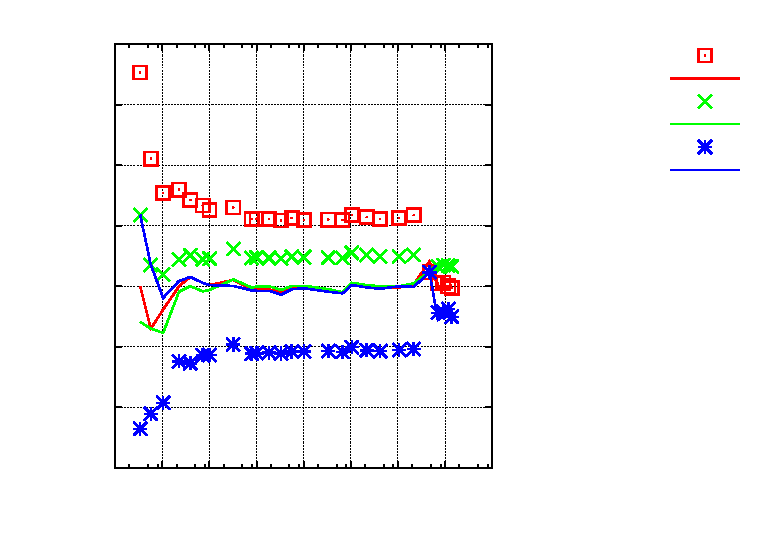
\includegraphics{../GNU/MegaAuto}}%
    \gplfronttext
  \end{picture}%
\endgroup

\caption{Kondensator-Messfehler von drei ATmega, vor und nach der Kalibration}
\label{fig:MegaAuto}
\end{figure}
